\documentclass[11pt,openany]{book}

\usepackage[margin=1.02in,headheight=15pt]{geometry}
\usepackage{amsmath,amssymb,mathtools,amsthm}
\usepackage{booktabs,longtable,array,tabularx,multirow}
\usepackage{graphicx}
\usepackage{xcolor}
\usepackage{microtype}
\usepackage{enumitem}
\usepackage{listings}
\usepackage{fancyhdr}
\usepackage{hyperref}
\usepackage[nameinlink,capitalize,noabbrev]{cleveref}
\usepackage[most]{tcolorbox}
\usepackage{makeidx}
\usepackage{url}
\usepackage{bm}

% Suppress intentionally blank verso pages in the digital monograph.
\let\cleardoublepage\clearpage

\graphicspath{{figures/}}
\makeindex
\setlist[itemize]{leftmargin=2em,itemsep=2pt,topsep=4pt}
\setlist[enumerate]{leftmargin=2.2em,itemsep=2pt,topsep=4pt}
\setcounter{tocdepth}{2}
\setcounter{secnumdepth}{3}
\numberwithin{equation}{chapter}
\emergencystretch=1.5em

\definecolor{restrictedblue}{HTML}{355C7D}
\definecolor{ambientrose}{HTML}{C06C84}
\definecolor{provedgreen}{HTML}{E8F8F5}
\definecolor{computedblue}{HTML}{EAF2F8}
\definecolor{skeletonyellow}{HTML}{FEF9E7}
\definecolor{conjecturered}{HTML}{FDEDEC}
\definecolor{ink}{HTML}{263238}

\hypersetup{
  colorlinks=true,
  linkcolor=restrictedblue,
  citecolor=restrictedblue,
  urlcolor=ambientrose,
  pdftitle={Catalytic Gate-Set Distortion: Temporary Escape in Quantum and Reversible Circuits},
  pdfauthor={Komorebi P.},
  pdfsubject={Symbolic, algebraic, and computational framework for restricted versus ambient gate complexity},
  pdfkeywords={quantum circuits, CNOT, Clifford, Toffoli, catalytic shortcut, word metric, holonomy, gate-set distortion, exact synthesis}
}

\pagestyle{fancy}
\fancyhf{}
\fancyhead[LE]{\small\thepage\quad\nouppercase{\leftmark}}
\fancyhead[RO]{\small\nouppercase{\rightmark}\quad\thepage}
\renewcommand{\headrulewidth}{0.3pt}

\newtheorem{theorem}{Theorem}[chapter]
\newtheorem{proposition}[theorem]{Proposition}
\newtheorem{lemma}[theorem]{Lemma}
\newtheorem{corollary}[theorem]{Corollary}
\newtheorem{principle}[theorem]{Principle}
\theoremstyle{definition}
\newtheorem{definition}[theorem]{Definition}
\newtheorem{example}[theorem]{Example}
\newtheorem{algorithm}[theorem]{Algorithm}
\newtheorem{protocol}[theorem]{Protocol}
\theoremstyle{remark}
\newtheorem{remark}[theorem]{Remark}
\newtheorem{question}[theorem]{Question}
\newtheorem{conjecture}[theorem]{Conjecture}

\newtcolorbox{provedbox}[1][]{colback=provedgreen,colframe=restrictedblue,title={Proved statement},fonttitle=\bfseries,#1}
\newtcolorbox{computedbox}[1][]{colback=computedblue,colframe=restrictedblue,title={Exact finite computation},fonttitle=\bfseries,#1}
\newtcolorbox{skeletonbox}[1][]{colback=skeletonyellow,colframe=orange!60!black,title={Formal research skeleton},fonttitle=\bfseries,#1}
\newtcolorbox{conjecturebox}[1][]{colback=conjecturered,colframe=ambientrose,title={Conjectural frontier},fonttitle=\bfseries,#1}
\newtcolorbox{boundarybox}[1][]{colback=gray!7,colframe=gray!65,title={Scope boundary},fonttitle=\bfseries,#1}

\lstdefinestyle{pythonstyle}{
 language=Python,
 basicstyle=\ttfamily\small,
 keywordstyle=\color{restrictedblue}\bfseries,
 commentstyle=\color{gray!70!black},
 stringstyle=\color{ambientrose},
 showstringspaces=false,
 breaklines=true,
 frame=single,
 rulecolor=\color{gray!40},
 columns=fullflexible
}
\lstdefinestyle{cppstyle}{
 language=C++,
 basicstyle=\ttfamily\small,
 keywordstyle=\color{restrictedblue}\bfseries,
 commentstyle=\color{gray!70!black},
 stringstyle=\color{ambientrose},
 showstringspaces=false,
 breaklines=true,
 frame=single,
 rulecolor=\color{gray!40},
 columns=fullflexible
}

\newcommand{\F}{\mathbb F}
\newcommand{\C}{\mathbb C}
\newcommand{\R}{\mathbb R}
\newcommand{\Z}{\mathbb Z}
\newcommand{\N}{\mathbb N}
\newcommand{\GL}{\operatorname{GL}}
\newcommand{\SL}{\operatorname{SL}}
\newcommand{\Sp}{\operatorname{Sp}}
\newcommand{\Egrp}{\operatorname{E}}
\newcommand{\U}{\operatorname{U}}
\newcommand{\Mat}{\operatorname{Mat}}
\newcommand{\Span}{\operatorname{span}}
\newcommand{\rank}{\operatorname{rank}}
\newcommand{\ord}{\operatorname{ord}}
\newcommand{\supp}{\operatorname{supp}}
\newcommand{\codim}{\operatorname{codim}}
\newcommand{\Prob}{\mathbb P}
\newcommand{\Exp}{\mathbb E}
\newcommand{\id}{I}
\newcommand{\ellDown}{\ell_{\downarrow}}
\newcommand{\ellAll}{\ell_{*}}
\newcommand{\ellBudget}[1]{\ell_{\le #1}}
\newcommand{\ellWeight}[1]{\ell_{#1}}
\newcommand{\tauGate}[3]{\tau_{#1,#2}(#3)}
\newcommand{\ellExc}[2]{\ell^{(#1,#2)}}
\newcommand{\ellRes}{\ell_{\mathrm{res}}}
\newcommand{\ellAmb}{\ell_{\mathrm{amb}}}
\newcommand{\DeltaDef}{\Delta}
\newcommand{\Gate}{\mathsf G}
\newcommand{\Res}{\mathsf R}
\newcommand{\Amb}{\mathsf A}
\newcommand{\cost}{\operatorname{cost}}
\newcommand{\Syn}{\operatorname{Syn}}
\newcommand{\Cliff}{\operatorname{Cliff}}
\newcommand{\Pauli}{\mathcal P}
\newcommand{\CX}{\operatorname{CX}}
\newcommand{\CZ}{\operatorname{CZ}}
\newcommand{\SWAP}{\operatorname{SWAP}}
\newcommand{\SUM}{\operatorname{SUM}}
\newcommand{\TOF}{\operatorname{TOF}}
\newcommand{\diag}{\operatorname{diag}}
\newcommand{\Aff}{\mathbb A}
\newcommand{\ket}[1]{\lvert #1\rangle}
\newcommand{\bra}[1]{\langle #1\rvert}
\newcommand{\braket}[2]{\langle #1\mid #2\rangle}

\title{\Huge Catalytic Gate-Set Distortion\\[0.5em]
\Large Temporary Escape in Quantum and Reversible Circuits\\[1em]
\large A Symbolic, Algebraic, and Computational Monograph}
\author{Komorebi P.}
\date{August 2026}

\begin{document}
\frontmatter
\maketitle

\chapter*{Abstract}
\addcontentsline{toc}{chapter}{Abstract}
This monograph develops a general theory of \emph{catalytic gate-set distortion}: a target belongs to a restricted circuit model, yet a shorter ambient realization temporarily leaves that model, reuses the resulting resource, and returns with the resource fully removed.  The framework covers metric defects, where both realizations exist but have different costs, and existence defects, where the restricted realization is impossible.  It treats scalar and vector resource costs, subgroup and groupoid holonomy, first-arrival Green kernels, algebraic product loci, border effects, tensor regularization, representable matroids, quiver factorizations, and root-system commutators.

The established linear core is reproduced in full.  A universal six-row transvection target has intrinsic length seven and ambient length six over every nonzero commutative ring with identity.  Connected families show that two reverse-directed gates can save linearly many gates, while tensor products yield an additive separation of order $n\log n$.  At fixed dimension, generic targets are rigid and defect-$d$ loci have codimension at least $d$.

The monograph then extends the program to quantum gate logic.  Modular SUM gates inherit the universal atom for every qudit dimension.  New exact finite computations are supplied for a symplectic Clifford model: in the swap-free primitive-count metric the parabolic subgroup is rigid through two qubits and has twenty-four defective targets at three qubits, whereas an entangling-count metric already has four two-qubit defects and $1624$ three-qubit defects.  Adding SWAP as a unit-cost primitive removes all three-qubit total-count defects.  By contrast, exhaustive three-bit enumeration finds no affine target shortened by adding Toffoli gates, under either total-count or entangling-count cost.  These results illustrate that defects depend essentially on the target class, gate alphabet, ancilla convention, and cost vector.

The remaining chapters give rigorous symbolic skeletons for CSS and Clifford synthesis, affine-to-nonlinear reversible logic, Clifford+$T$ and phase-polynomial circuits, Gaussian and fermionic systems, symmetry-preserving circuits, measurement and feedforward, architecture constraints, and finite packet or realization hierarchies.  Proved statements, exact computations, formal skeletons, and conjectures are visibly separated throughout.  The accompanying Python and C++ atlas reproduces the finite experiments and provides reusable search, certificate, and circuit-drawing components.

\chapter*{Reader's guide and status convention}
\addcontentsline{toc}{chapter}{Reader's guide and status convention}
The scope is intentionally broad, but the logical status is not blurred.  Green boxes contain symbolic proofs or consequences of stated hypotheses.  Blue boxes contain complete finite computations with an explicit state model and exhaustive search.  Yellow boxes specify a mathematically complete research skeleton whose decisive lower bound or classification remains open.  Red boxes state conjectures or candidate mechanisms.  A statement in a yellow or red box is not promoted to a theorem elsewhere in the text.

\begin{figure}[ht]
\centering
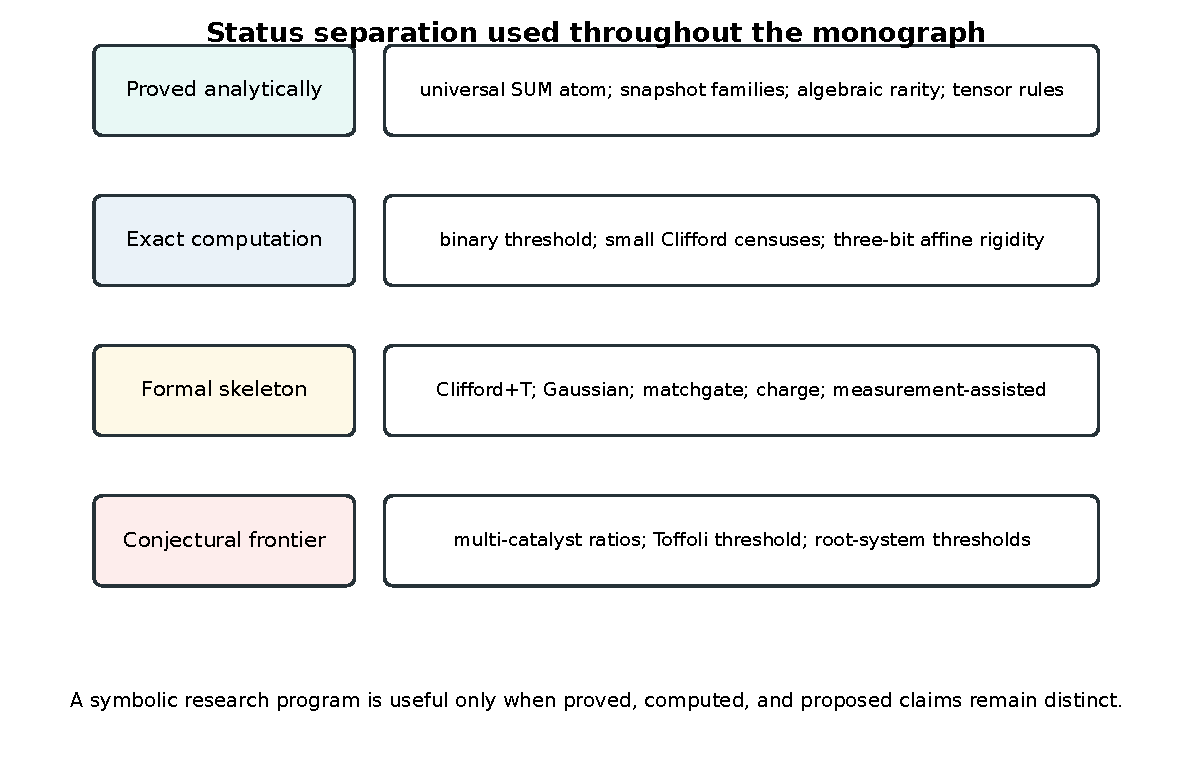
\includegraphics[width=.92\textwidth]{status_map.pdf}
\caption{The status separation used throughout the monograph.}
\end{figure}

The established unitriangular paper is incorporated as a complete core chapter rather than paraphrased.  Its computer-assisted claims retain their original finite-state completeness conditions.  The new Clifford and affine-versus-Toffoli computations use exact binary symplectic matrices and exact permutations, respectively.  Quantum Latin squares enter only as a contextual example of an existence defect; no circuit theorem is inferred from that example.

\chapter*{Notation and recurring objects}
\addcontentsline{toc}{chapter}{Notation and recurring objects}
\begin{longtable}{@{}p{.22\textwidth}p{.70\textwidth}@{}}
\toprule
Symbol & Meaning\\
\midrule
$H\le G$ & Restricted and ambient groups, when both models are group generated.\\
$\mathcal S_H\subseteq\mathcal S_G$ & Restricted and ambient elementary gate alphabets.\\
$\ellRes(U),\ellAmb(U)$ & Minimum restricted and ambient costs of a target $U$.\\
$\Delta(U)$ & Gate-set defect $\ellRes(U)-\ellAmb(U)$, with $+\infty$ allowed for existence defects.\\
$D_n$ & Worst additive defect at size $n$.\\
$R_n$ & Worst multiplicative distortion at size $n$.\\
$A_S$ & Convolution or adjacency operator associated with a finite generator set $S$.\\
$\mathcal G_{S,U}(z)$ & Endpoint Green kernel $\langle\delta_U,(I-zA_S)^{-1}\delta_e\rangle$.\\
$P_n$ & Binary symplectic parabolic subgroup preserving the $Z$ Lagrangian.\\
$\tau_\otimes$ & Stable tensor-normalized ambient cost.\\
$\kappa_\otimes$ & Stable catalytic tensor capacity.\\
\bottomrule
\end{longtable}

\tableofcontents
\listoffigures
\begingroup
\renewcommand{\addvspace}[1]{}
\listoftables
\endgroup

\mainmatter

\part{General theory of temporary escape}
\chapter{Nested gate models and distortion invariants}\label{ch:nested-models}
\index{gate-set distortion}
\index{restricted realization}
\index{ambient realization}
\index{cost vector}
\index{existence defect}


\section{Why a separate theory is needed}
A target transformation often belongs to a visibly structured class even when the machine used to realize it is capable of much more.  A lower-triangular linear transformation may be synthesized by an unrestricted CNOT network.  A diagonal unitary may be realized by a non-diagonal Clifford+$T$ circuit.  A charge-preserving unitary may be compiled by gates that temporarily visit other charge sectors.  A Gaussian target may be realized by a circuit that briefly uses a non-Gaussian primitive.  These situations share a question that is not answered by ordinary exact synthesis:
\begin{quote}
How much does it cost to require the \emph{entire path} of a computation to retain the structure possessed by its endpoint?
\end{quote}
The distinction is path dependent.  It is not determined only by membership of the final target in a subgroup, a subcategory, or a model class.

\begin{figure}[ht]
\centering
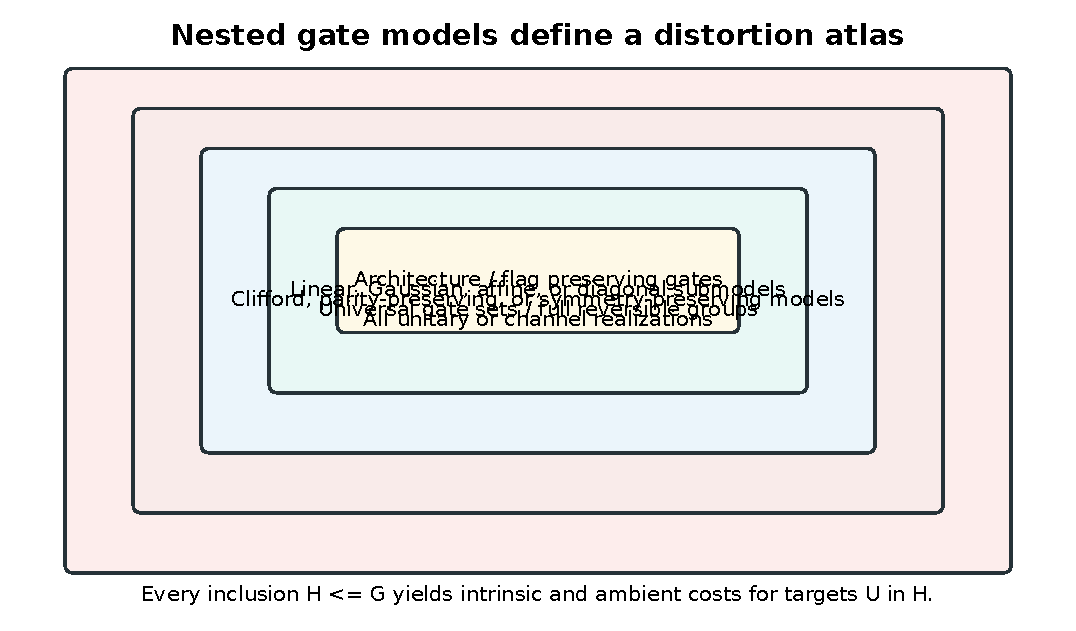
\includegraphics[width=.90\textwidth]{gate_hierarchy.pdf}
\caption{Representative nested gate models.  The same target can be assigned different costs at several levels.}
\label{fig:gate-hierarchy}
\end{figure}

\section{Exact gate models}
\begin{definition}[Gate model]
An \emph{exact gate model} is a tuple
\[
\mathfrak M=(\mathcal X,\mathcal S,c,\circ),
\]
where $\mathcal X$ is a set of states or morphisms, $\mathcal S$ is a specified family of elementary generators, $c:\mathcal S\to\R_{\ge0}$ is a cost function, and $\circ$ is the composition law.  A word
\[
w=s_L\cdots s_1
\]
has cost
\[
c(w)=\sum_{j=1}^L c(s_j).
\]
For a target $U\in\mathcal X$, the exact synthesis cost is
\[
\ell_{\mathfrak M}(U)=\inf\{c(w):w=U\}.
\]
The value is $+\infty$ when the target has no realization.
\end{definition}

The composition law may be group multiplication, composition of permutations, composition of quantum channels, tensor-network contraction, or composition in a dagger symmetric monoidal category.  The additive cost may count all gates, only entangling gates, only non-Clifford gates, weighted error, or a vector of several resources.  Depth fits this additive model by taking admissible parallel layers as generators, rather than charging one unit to each individual gate.

\begin{definition}[Nested realization pair]
A \emph{nested realization pair} consists of restricted and ambient models
\[
\mathfrak M_{\mathrm{res}}\subseteq\mathfrak M_{\mathrm{amb}}
\]
with a common target class $\mathcal T$ of finite ambient cost and the same cost on common generators.  For $U\in\mathcal T$, define
\[
\ellRes(U)=\ell_{\mathfrak M_{\mathrm{res}}}(U),
\qquad
\ellAmb(U)=\ell_{\mathfrak M_{\mathrm{amb}}}(U).
\]
The additive defect is
\[
\Delta(U)=\ellRes(U)-\ellAmb(U).
\]
\end{definition}

When both costs are finite, $\Delta(U)$ is a metric or optimization defect.  If $\ellRes(U)=+\infty$ and $\ellAmb(U)<+\infty$, it is an existence defect.  This convention unifies finite gate savings with the failure of a restricted realization category.

\begin{proposition}[Monotonicity]
For every target in the common domain,
\[
\ellAmb(U)\le \ellRes(U).
\]
Consequently $\Delta(U)\ge0$ whenever both models use the same nonnegative cost on their common generators.
\end{proposition}
\begin{proof}
Every restricted word is also an ambient word.
\end{proof}

\section{Cost models are part of the theorem}
A gate-set comparison is incomplete until the cost convention is fixed.  The same pair of groups can display a defect under entangling count and no defect under total primitive count.  A SWAP gate may be primitive, may cost three CNOTs, or may be implemented by physical motion.  A local Clifford may be free in a fault-tolerant resource estimate and nonfree in a pulse-level model.

\begin{definition}[Resource vector]
Let
\[
\mathbf c(s)=(c_1(s),\ldots,c_r(s))\in\R_{\ge0}^r
\]
be the resource vector of a gate.  The achievable resource region of a target is
\[
\mathcal P_{\mathfrak M}(U)
=
\left\{
\sum_{j=1}^L\mathbf c(s_j):s_L\cdots s_1=U
\right\}.
\]
Its nondominated points form the Pareto boundary.
\end{definition}

For a weight vector $\lambda\in\R_{\ge0}^r$, scalarization gives
\[
\ell_{\mathfrak M}^{\lambda}(U)
=
\inf_{x\in\mathcal P_{\mathfrak M}(U)}\lambda\cdot x.
\]
The scalar defect $\Delta^\lambda(U)$ can vary with $\lambda$ even when the target and gate alphabets are fixed.

\begin{figure}[ht]
\centering
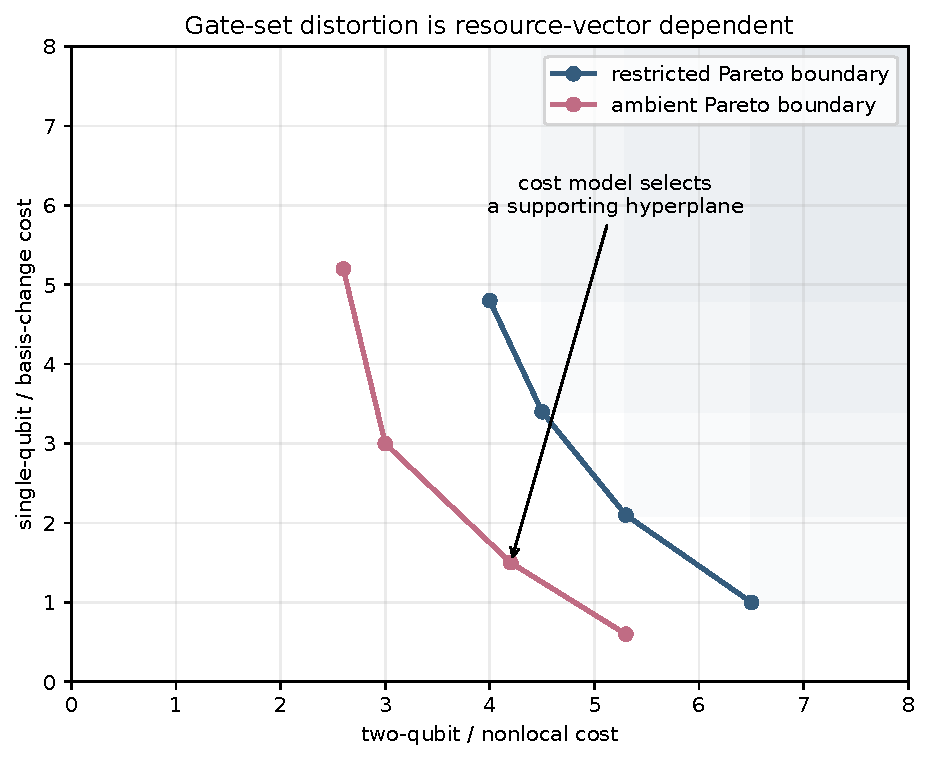
\includegraphics[width=.74\textwidth]{resource_pareto.pdf}
\caption{Restricted and ambient Pareto regions can differ without one model dominating by the same amount under every resource weighting.}
\label{fig:pareto}
\end{figure}

\begin{principle}[Model specificity]
Every claimed shortcut must state the target class, elementary gate alphabet, ancilla convention, exact or approximate synthesis criterion, and cost vector.  Changing any one of these may remove, create, or reverse a defect.
\end{principle}

\section{Ancilla and restoration conventions}
Temporary workspace is meaningful only after its restoration rule is specified.
\begin{definition}[Ancilla conventions]
An ancilla is
\begin{enumerate}
\item \emph{clean} if it begins in a specified state and must return to that state,
\item \emph{borrowed} or \emph{dirty} if its initial state is arbitrary but must be restored,
\item \emph{consumable} if restoration is not required,
\item \emph{catalytic} if it is restored while enabling a cheaper realization of the target.
\end{enumerate}
\end{definition}
The present theory focuses on restoration.  If an auxiliary resource may be discarded, the comparison becomes a different channel or isometry synthesis problem.

\section{Worst-case and threshold functions}
For a size parameter $n$, let $\mathcal T_n$ denote the target family.
\begin{definition}[Extremal distortion]
Define
\[
D_n=\sup_{U\in\mathcal T_n}\Delta(U)
\]
and, when $0<\ellAmb(U)<\infty$,
\[
R_n=\sup_{U\in\mathcal T_n}
\frac{\ellRes(U)}{\ellAmb(U)}.
\]
The first defective size is
\[
\tau=\min\{n:D_n>0\}.
\]
We set a threshold to $+\infty$ when its defining set is empty.
\end{definition}

Several threshold notions should not be conflated:
\begin{align*}
\tau_{\mathrm{metric}}&=\min\{n:\exists U,\ 0<\Delta(U)<\infty\},\\
\tau_{\mathrm{exist}}&=\min\{n:\exists U,\ \ellRes(U)=\infty,\ \ellAmb(U)<\infty\},\\
\tau_{q}&=\min\{n:\exists U,\ \ell_{\le q}(U)<\ell_{\le0}(U)\},
\end{align*}
where $\ell_{\le q}$ permits at most $q$ ambient-only gates.  A model may have an early metric threshold and a later existence threshold, or no threshold at all.

\section{Equivalence, orbits, and classification}
A finite census should be quotiented by transformations preserving both gate models and the cost.  Depending on the problem, these may include wire permutations, local Clifford conjugation, isotopy, simultaneous row and column relabeling, or graph automorphisms.

\begin{definition}[Cost-preserving equivalence]
Targets $U$ and $V$ are equivalent if an automorphism $\varphi$ of the ambient realization system satisfies
\[
\varphi(U)=V,
\qquad
\varphi(\mathcal S_{\mathrm{res}})=\mathcal S_{\mathrm{res}},
\qquad
\varphi(\mathcal S_{\mathrm{amb}})=\mathcal S_{\mathrm{amb}},
\]
and preserves the gate costs.
\end{definition}
Under this equivalence, both lengths and the defect are orbit invariants.  A useful threshold theorem should classify minimal defective orbits, not merely list raw matrices.

\section{Approximate synthesis and border defects}
For continuous gate models, exact word length can differ from the minimum length achievable as a limit.
\begin{definition}[Border cost]
Let $\overline{\mathcal W}_{L}$ be the topological or Zariski closure of targets realizable with cost at most $L$.  The border cost is
\[
\underline\ell(U)=\inf\{L:U\in\overline{\mathcal W}_{L}\}.
\]
The border defect is
\[
\underline\Delta(U)=
\underline\ell_{\mathrm{res}}(U)-
\underline\ell_{\mathrm{amb}}(U).
\]
\end{definition}
This is the circuit analogue of the distinction between tensor rank and border rank.  An exact defect can disappear under degeneration, persist, or become larger after approximation changes the relevant cost geometry.

\section{Metric and existence defects in one category}
Let $\mathcal C_{\mathrm{res}}\subseteq\mathcal C_{\mathrm{amb}}$ be categories with weighted generating morphisms.  For a morphism $f$ in the restricted target class, the same definition
\[
\Delta(f)=c_{\mathrm{res}}(f)-c_{\mathrm{amb}}(f)
\]
includes group-word metrics, adaptive quantum channels, tensor-network realizations, and orthogonality designs.  This categorical form is essential when the ambient model permits measurement, branching, postselection, or entangled objects that do not lie in a common group.

\begin{boundarybox}
The abstract definition does not prove that a defect exists.  It provides a common language in which a finite search, a symbolic identity, and a lower-bound certificate can be compared without changing the meaning of the target or the cost.
\end{boundarybox}

\section{A standard theorem package}
A mature gate-set distortion result should contain as many of the following components as the model allows:
\begin{enumerate}
\item a precisely defined nested gate pair and cost vector,
\item a smallest defective target or a no-defect theorem below a threshold,
\item an explicit ambient word,
\item a restricted lower-bound certificate,
\item classification modulo cost-preserving equivalence,
\item a reusable catalytic normal form,
\item direct-sum, recursive, or tensor amplification,
\item generic-rigidity or sparsity results,
\item a certificate-producing implementation,
\item a clear account of which statements are symbolic, computed, or conjectural.
\end{enumerate}
The remainder of the monograph follows this package.

\chapter{Catalytic holonomy, excursion geometry, and resource reuse}\label{ch:holonomy}
\index{holonomy}
\index{Schreier graph}
\index{catalytic conjugation}
\index{dirty workspace}
\index{resource amortization}


\section{Subgroup metrics and Schreier loops}
Assume first that the restricted and ambient models are groups
\[
H=\langle\mathcal S_H\rangle
\le
G=\langle\mathcal S_G\rangle.
\]
For $h\in H$, the intrinsic and ambient word metrics are
\[
\ell_H(h)=|h|_{\mathcal S_H},
\qquad
\ell_G(h)=|h|_{\mathcal S_G}.
\]
In the group-metric statements, the generating alphabets are symmetric and a generator and its inverse have equal cost.  The quotient geometry is the left Schreier graph $G/H$, with edges $gH\longmapsto sgH$.  For the base-fiber assertion below, assume also $\mathcal S_H=\mathcal S_G\cap H$.  This last condition excludes additional ambient primitives that already lie in $H$ but have no equally cheap restricted realization.

\begin{theorem}[Holonomy-compression identity]
Let every generator have unit cost.  For $h\in H$, $\ell_G(h)$ is the minimum length of a based loop in $G/H$ whose lifted word has holonomy $h$.  The intrinsic length $\ell_H(h)$ is the minimum length among loops that remain in the base fiber.
\end{theorem}
\begin{proof}
An ambient word $s_k\cdots s_1=h$ projects to the loop
\[
H,
s_1H,
s_2s_1H,
\ldots,
hH=H.
\]
Conversely, a based Schreier loop has product in $H$.  If every prefix lies in $H$, each edge label is the product of two elements of $H$ and belongs to $\mathcal S_G\cap H=\mathcal S_H$.  Conversely every restricted word remains in the base fiber.  Minimizing the labeled words with endpoint $h$ gives the two asserted lengths.
\end{proof}

Thus
\[
\Delta_{H\hookrightarrow G}(h)
=
\text{intrinsic fiber cost}
-
\text{shortest holonomy loop cost}.
\]
This is the geometric content of a dirty-workspace shortcut.

\begin{figure}[ht]
\centering
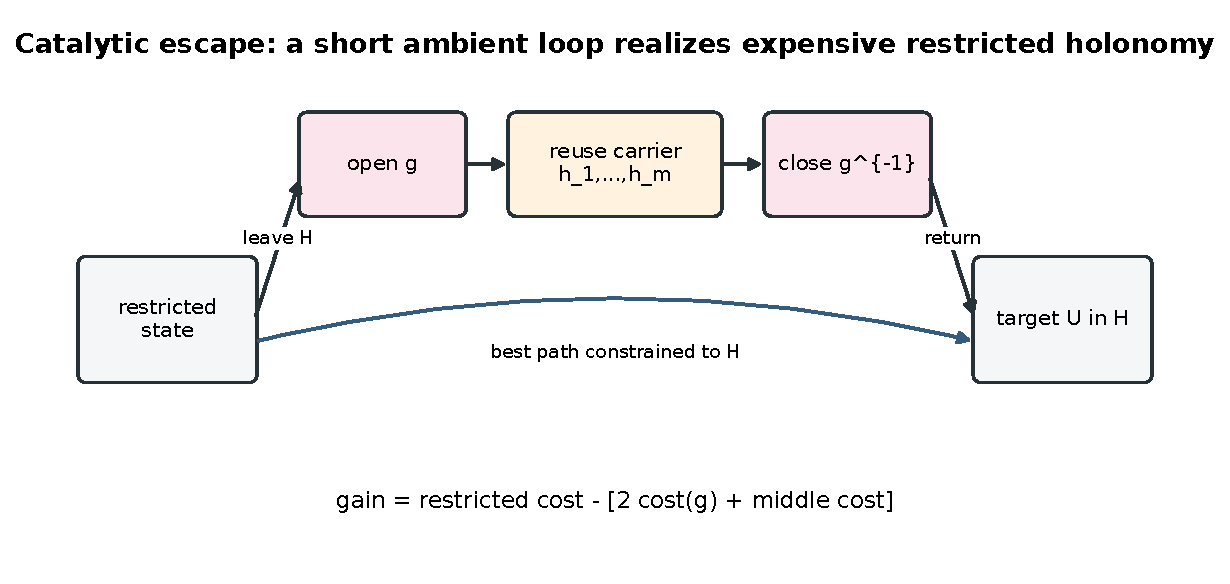
\includegraphics[width=.90\textwidth]{catalytic_excursion_general.pdf}
\caption{A catalytic excursion leaves a restricted fiber, reuses an ambient state, and returns with nontrivial holonomy.}
\label{fig:catalytic-excursion}
\end{figure}

\section{The basic conjugation inequality}
Let $g\in G$ and $k\in H$ satisfy $gkg^{-1}\in H$.  Then
\[
\ell_G(gkg^{-1})
\le 2\ell_G(g)+\ell_H(k).
\]
Define the intrinsic conjugation stretch
\[
\operatorname{Stretch}_g(k)
=
\ell_H(gkg^{-1})-\ell_H(k).
\]

\begin{proposition}[Catalytic stretch criterion]
If
\[
\operatorname{Stretch}_g(k)>2\ell_G(g),
\]
then $gkg^{-1}$ has positive defect.
\end{proposition}
The opening and closing cost is paid once.  Every useful consumer inside the excursion contributes to the stretch.

\section{Many consumers and catalytic excess}
Suppose the middle word is
\[
k=h_m\cdots h_1,
\qquad h_i\in H.
\]
The ambient word
\[
gh_m\cdots h_1g^{-1}
\]
has cost at most
\[
2c(g)+\sum_i c(h_i).
\]
If the restricted images $gh_ig^{-1}$ require costs $r_i$ and a lower-bound invariant proves that their obligations cannot be shared, then
\[
\ell_H(gkg^{-1})\ge\sum_i r_i.
\]
A sufficient inequality is
\[
\sum_i(r_i-c(h_i))>2c(g).
\]
The left side is the gross catalytic benefit.  The right side is the restoration cost.

\begin{definition}[Catalytic excess]
For a normal form with $r$ matched excursions and $C$ useful cross interactions, define
\[
\mathcal E=C-2r
\]
when each consumer contributes one unit and each opening or closing costs one unit.
\end{definition}
Positive excess is necessary in the simplest transvection model, but it is not sufficient.  An all-cross configuration may admit a mirror word of equal restricted length.  Temporal asymmetry or phase holonomy is also required.

\section{Excursion budgets}
Counting ambient-only gates is only one measure of how far a circuit leaves its restricted model.
\begin{definition}[Excursion profile]
For a circuit path $X_0,X_1,\ldots,X_L$, an excursion profile may include
\begin{enumerate}
\item the number $q$ of ambient-only gates,
\item the maximum Schreier distance $d(X_tH,H)$,
\item the rank of a forbidden block,
\item the bandwidth of a forbidden dependency,
\item the number of simultaneously open catalytic intervals,
\item the intersection graph of those intervals,
\item the maximum algebraic degree created temporarily,
\item the maximum ancilla dimension or branch count.
\end{enumerate}
\end{definition}
The established linear family shows that a rank-one, bandwidth-one excursion using exactly two forbidden gates can save linearly many operations.  Thus geometric excursion size need not control computational benefit.

\section{Catalytic interval geometry}
Associate to every matched opening and closing operation an interval
\[
I_j=[t_j^{\mathrm{open}},t_j^{\mathrm{close}}].
\]
The family of intervals can be disjoint, nested, laminar, or crossing.

\begin{principle}[First higher-order frontier]
Independent or disjoint intervals often reduce to additive copies of a one-catalyst analysis.  Crossing intervals are the first place where one dirty resource can alter another and where a multiplicative distortion larger than the clean one-carrier value may occur.
\end{principle}

Define the catalytic width
\[
w_{\mathrm{cat}}=
\max_t
\#\{j:t\in I_j\}.
\]
One may then study
\[
D_n^{(w)}
=
\max_{U}
\left(
\ellRes(U)-\ellAmb^{(w)}(U)
\right),
\]
where the ambient circuit has width at most $w$.  The unitriangular snapshot family gives $D_n^{(1)}=\Omega(n)$ in its corresponding interval model.

\section{Four recurrent catalytic mechanisms}
\subsection{Basis-change catalysis}
An ambient gate $g$ changes the frame in which several restricted operations are cheap:
\[
h_i\mapsto gh_ig^{-1}.
\]
Hadamard and Fourier transforms are the basic quantum examples.  The frame is restored at the end.

\subsection{Commutator catalysis}
An ambient commutator creates a new direction:
\[
[g,h]=ghg^{-1}h^{-1}.
\]
For continuous controls,
\[
e^{\varepsilon X}e^{\varepsilon Y}e^{-\varepsilon X}e^{-\varepsilon Y}
=
e^{\varepsilon^2[X,Y]+O(\varepsilon^3)}.
\]
The desired effective generator may lie in the restricted algebra even though the path does not.

\subsection{Degree catalysis}
A Toffoli, CCZ, or non-Gaussian gate can create higher algebraic degree or higher moments temporarily.  If the nonlinear object is reused and canceled, the final target may remain affine, diagonal, or Gaussian.

\subsection{Branch and workspace catalysis}
Ancillas, measurements, reset, teleportation, and classical feedforward enlarge the realization category.  The resource is a temporary branch, subsystem, or borrowed state rather than a group element.

\section{When defects are impossible}
A useful positive theorem is a criterion guaranteeing geodesic convexity.
\begin{proposition}[One-Lipschitz retraction criterion]
Suppose there is a group homomorphism $\pi:G\to H$ with $\pi|_H=\operatorname{id}_H$ such that every ambient generator $s\in\mathcal S_G$ satisfies
\[
\ell_H(\pi(s))\le c(s).
\]
Then
\[
\ell_H(h)\le\ell_G(h)
\]
for every $h\in H$, hence the two metrics agree on $H$.
\end{proposition}
\begin{proof}
For an ambient word $h=s_L\cdots s_1$, multiplicativity gives $h=\pi(h)=\pi(s_L)\cdots\pi(s_1)$.  Subadditivity and the generator bounds give $\ell_H(h)\le\sum_j c(s_j)$.  Taking the infimum over ambient words proves the claim.
\end{proof}

The unitriangular counterexample proves that no such generator-wise one-Lipschitz retraction exists for the lower transvection model inside the all-transvection model.

\section{Weighted restoration and phase transitions}
Let every restricted gate cost one and every ambient-only gate cost $\lambda$.  For a catalyst used by $v$ consumers with unit benefit, the displayed construction has net gain at least
\[
v-2\lambda.
\]
The critical weight is therefore target and mechanism dependent.

\begin{definition}[Critical catalyst penalty]
For a target family $U_n$, define
\[
\lambda_c(U_n)
=
\sup\{\lambda:\ell_{\lambda,\mathrm{amb}}(U_n)<\ellRes(U_n)\}.
\]
\end{definition}
Determining $\lambda_c$ exactly is a refined synthesis problem.  It can be more physically meaningful than unweighted gate count.

\section{Restoration is the source of nontriviality}
If the ambient resource need not be restored, the opening cost can dominate the comparison and many examples become trivial.  Catalytic escape is strongest when the following all hold:
\begin{enumerate}
\item the final target lies entirely in the restricted class,
\item every auxiliary subsystem or violated constraint is restored,
\item the ambient-only resource is used more than once,
\item the restricted lower bound charges the same repeated obligations separately,
\item the gain survives a realistic weighted cost.
\end{enumerate}

\begin{conjecturebox}
In many finite gate hierarchies, minimal defects should admit a bounded-width catalytic normal form.  Proving or refuting this would turn an unrestricted synthesis search into a search over a finite family of excursion motifs.
\end{conjecturebox}

\chapter{First arrival, spectral packets, algebraic rarity, and tensor regularization}\label{ch:spectral-algebraic}
\index{Green kernel}
\index{first-arrival valuation}
\index{word map}
\index{algebraic defect locus}
\index{border rank}
\index{tensor capacity}


\section{Word distance as first arrival}
Let $G$ be finite and let $S=S^{-1}$ be a symmetric generating multiset.  In the right regular representation, define
\[
A_S=\sum_{s\in S}\rho(s).
\]
Then
\[
\langle\delta_g,A_S^k\delta_e\rangle
\]
counts length-$k$ words ending at $g$.

\begin{theorem}[Endpoint Green valuation]
The word distance is
\[
d_S(e,g)
=
\ord_{z=0}
\left\langle
\delta_g,(I-zA_S)^{-1}\delta_e
\right\rangle.
\]
\end{theorem}
\begin{proof}
Expand the resolvent as a formal power series:
\[
(I-zA_S)^{-1}=\sum_{k\ge0}z^kA_S^k.
\]
The first nonzero endpoint coefficient occurs at the shortest word length.
\end{proof}

For strictly positive integer costs, replace each generator $s$ by the monomial $z^{c(s)}\rho(s)$.  Every coefficient then counts finitely many words of a given total cost, and the same formal inverse is defined.  Zero-cost cycles require separate treatment: they can create infinitely many words of cost zero, so the ordinary counting series need not exist.  The finite atlases with free gates use shortest-path search with zero-cost edges instead.  Multivariate variables can track several resources when the grading gives every generator positive total degree.

\section{Why eigenvalues alone are insufficient}
If
\[
A_S=\sum_\lambda\lambda\Pi_\lambda,
\]
then
\[
\mathcal G_{S,g}(z)
=
\sum_\lambda
\frac{\langle\delta_g,\Pi_\lambda\delta_e\rangle}{1-\lambda z}.
\]
The eigenvalues and multiplicities do not determine the endpoint coefficients
\[
\langle\delta_g,\Pi_\lambda\delta_e\rangle.
\]
Two Cayley or Schreier systems can therefore be cospectral and still have different first-arrival behavior at distinguished targets.

\begin{principle}[Embedded packet principle]
For threshold questions, a spectral label is usually weaker than an embedded spectral projector.  The matrix coefficients of the projector relative to the initial and target states retain positional information that multiplicities erase.
\end{principle}

This distinction recurs in the Latin-square example discussed later.  The natural commuting row, column, and symbol operators have universal eigenvalue packets at fixed order, while the embedded incidence and transition data still vary.

\section{Subgroup-holonomy Fourier packets}
Let $H\le G$.  Let $\mu_k(h)$ count ambient words of length $k$ with product $h\in H$.  For every irreducible representation $\tau\in\widehat H$, define
\[
\widehat\mu_k(\tau)
=
\sum_{h\in H}\mu_k(h)\tau(h).
\]
Fourier inversion gives
\[
\mu_k(h)
=
\frac1{|H|}
\sum_{\tau\in\widehat H}
\dim(\tau)
\operatorname{tr}
\bigl(
\tau(h^{-1})\widehat\mu_k(\tau)
\bigr).
\]
The matrix-valued Green packet
\[
\widehat{\mathcal G}_\tau(z)
=
\sum_{k\ge0}\widehat\mu_k(\tau)z^k
\]
recovers every endpoint series after Fourier inversion.

The trivial representation records only the total number of loops returning to the subgroup.  Nontrivial $H$-types retain their holonomy.  This yields a hierarchy:
\[
\text{spherical return data}
\prec
\text{type-resolved holonomy packets}
\prec
\text{exact endpoint realization}.
\]

\section{Word maps and product loci}
Let $K$ be a field and let $X\subseteq G$ be an algebraic gate family.  For a fixed length $L$, multiplication defines
\[
\mu_L:X^L\to G,
\qquad
(x_L,\ldots,x_1)\mapsto x_L\cdots x_1.
\]
The exact length-$L$ locus is $\mu_L(X^L)$, and the length-at-most-$L$ locus is a finite union of such images when the gate family has finitely many components.

\begin{theorem}[Dimension per gate]
Suppose every irreducible component of $X$ has dimension at most $r$.  Then the Zariski closure of the locus reachable in at most $L$ gates has dimension at most $rL$.
\end{theorem}
\begin{proof}
Every component of $X^L$ has dimension at most $rL$.  A morphism cannot increase dimension.  A finite union has dimension equal to the maximum dimension of its components.
\end{proof}

For scaled transvections, $r=1$.  This immediately yields generic lower bounds in a target variety whose dimension exceeds $L$.

\section{Generic rigidity}
Work over an algebraically closed field.  Suppose the restricted target variety $V$ is irreducible of dimension $N$, every target has a restricted realization using at most $N$ unit-cost gates, and the ambient alphabet is an algebraic family with finitely many components of dimension at most one.  Then ambient realizations of length below $N$ occupy a proper closed subset of $V$.

\begin{theorem}[Abstract generic rigidity]
Under the preceding hypotheses, there is a nonempty Zariski-open subset $\Omega\subseteq V$ such that
\[
\ellRes(U)=\ellAmb(U)=N
\qquad(U\in\Omega).
\]
\end{theorem}
The unitriangular theorem in the core chapter is a concrete instance with
\[
N=\binom n2.
\]

\section{Defect codimension}
If every target has restricted cost at most $N$, then defect at least $d$ forces ambient cost at most $N-d$.  The dimension-per-gate theorem gives
\[
\codim_V\overline{\{U:\Delta(U)\ge d\}}
\ge d
\]
when each ambient gate carries one parameter.

\begin{principle}[Rare but amplifiable]
At fixed dimension, large defects require increasingly special algebraic conditions.  Under direct sums, recursive lifts, or tensor products, a point on a thin exceptional stratum can nevertheless seed a macroscopic family.
\end{principle}

This is one of the central tensions of the subject.  Catalysis is neither generic nor negligible.

\section{Finite-field sparsity}
A word-counting analogue applies over $\F_q$.  If the ambient alphabet has at most $M(q-1)$ nontrivial scaled gates, then the number of targets reached in $L$ gates is at most
\[
\sum_{j=0}^L[M(q-1)]^j.
\]
When the target space has $q^N$ points and defect $d$ implies ambient length at most $N-d$, the crude bound is
\[
\Prob[\Delta\ge d]
=O_{N,M}(q^{-d}).
\]
The estimate can be sharpened by orbit counting, stabilizers, and the geometry of word-map fibers.

\section{Direct sums and monoidal amplification}
Suppose targets admit a direct sum $U\oplus V$ and a homomorphism from the large restricted group onto the two factor groups sends $U\oplus V$ to $(U,V)$.  Require the aggregate generator bound
\[
\ellRes(\pi_1(s))+\ellRes(\pi_2(s))\le c(s)
\]
for every large restricted generator $s$.  Assume that both restricted and ambient factor circuits embed into the corresponding large model without increasing cost.  Then
\[
\ellRes(U\oplus V)
=
\ellRes(U)+\ellRes(V).
\]
Indeed, projecting any word and summing the two factor bounds gives the lower bound, while concatenating the embedded factor circuits gives the upper bound.  Separate one-Lipschitz projections alone do not imply this sum inequality.
Under the ambient embedding assumption, the constructive upper bound is
\[
\ellAmb(U\oplus V)
\le
\ellAmb(U)+\ellAmb(V),
\]
so
\[
\Delta(U\oplus V)
\ge
\Delta(U)+\Delta(V).
\]
One finite defect therefore gives an unbounded additive family.

\section{Tensor products and normalized rates}
Let $U$ have dimension $m$ and $V$ dimension $n$.  In linear transvection models with tree-tight certificates,
\[
\ellRes(U\otimes V)
=
n\ellRes(U)+m\ellRes(V).
\]
The ambient model satisfies the corresponding inequality.  Normalizing by dimension gives an entropy-like law:
\[
\frac{\ellRes(U\otimes V)}{mn}
=
\frac{\ellRes(U)}m+
\frac{\ellRes(V)}n.
\]
The normalized defect is superadditive under tensor products.

\begin{definition}[Tensor synergy]
Define
\[
\Syn(U,V)
=
n\ellAmb(U)+m\ellAmb(V)-\ellAmb(U\otimes V).
\]
Positive synergy means that the joint ambient realization improves on independent lifted circuits.
\end{definition}
Restricted tree-tight metrics have zero tensor synergy.  Ambient synergy is a possible source of collective activation.

\begin{definition}[Stable tensor cost]
For a size-$m$ target $U$, define
\[
\tau_\otimes(U)
=
\lim_{r\to\infty}
\frac{\ellAmb(U^{\otimes r})}{r m^{r-1}},
\]
when the subadditivity argument applies.  Define
\[
\kappa_\otimes(U)
=
\ellRes(U)-\tau_\otimes(U).
\]
\end{definition}
Fekete's lemma gives the limit from the tensor subadditivity inequality.

\begin{figure}[ht]
\centering
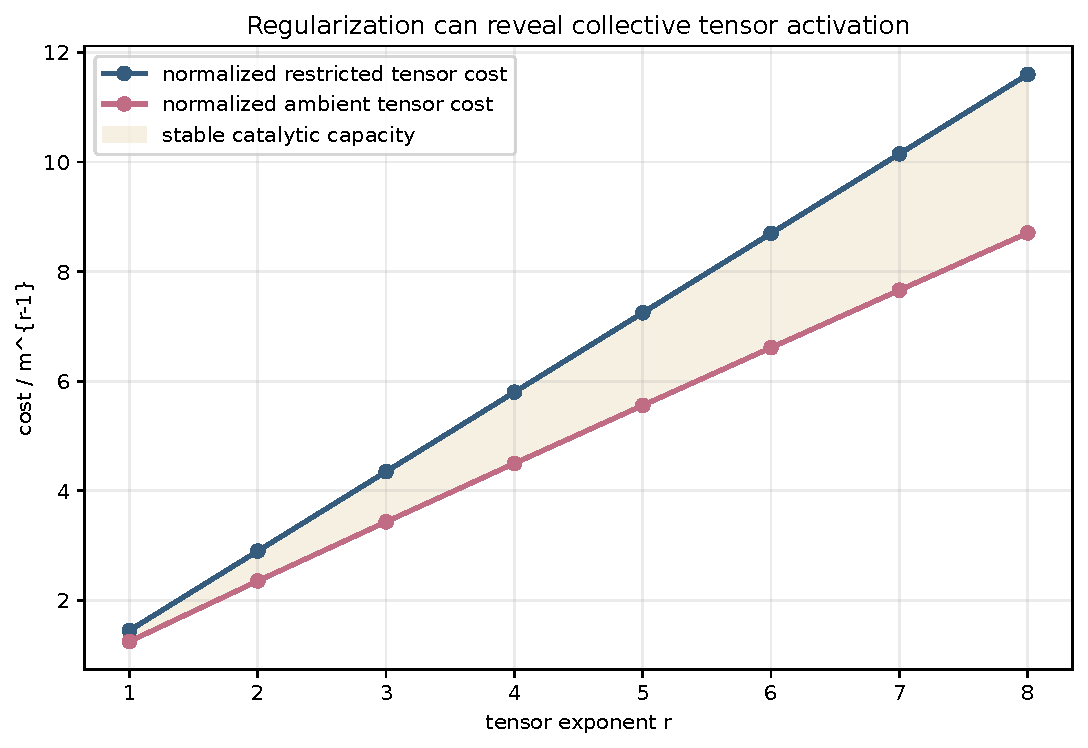
\includegraphics[width=.72\textwidth]{tensor_capacity.pdf}
\caption{Schematic stable tensor capacity.  The figure illustrates definitions, not measured data.}
\end{figure}

\begin{definition}[Tensor activation]
A target is tensor activated if
\[
\Delta(U)=0
\quad\text{but}\quad
\kappa_\otimes(U)>0.
\]
\end{definition}
This is analogous to regularized capacities and asymptotic ranks.  It asks whether collective synthesis can unlock a catalyst invisible in one copy.

\section{Border catalysis}
Let $X_{\mathrm{res}}$ and $X_{\mathrm{amb}}$ be algebraic gate varieties.  The exact product rank is
\[
\operatorname{rk}_{X}(U)
=
\min\{L:U\in X^L\},
\]
while border product rank is
\[
\underline{\operatorname{rk}}_{X}(U)
=
\min\{L:U\in\overline{X^L}\}.
\]
The four possible comparisons are:
\begin{enumerate}
\item exact and border defects both positive,
\item exact defect positive but border defect zero,
\item one-copy defect zero but tensor-regularized defect positive,
\item ambient and restricted border ranks both smaller than exact ranks but by different amounts.
\end{enumerate}
Each requires a separate certificate.  Numerical approximation alone does not distinguish them.

\section{A packet-resolved threshold principle}
Combining the preceding constructions gives the following architecture.
\begin{enumerate}
\item A coarse commutative algebra supplies spherical spectral packets.
\item Embedded projectors retain incidence and endpoint position.
\item Noncommutative transition data record holonomy.
\item A realization theorem decides whether the packet has a restricted representative and at what cost.
\item Direct sums and tensor products propagate local defects.
\end{enumerate}

\begin{figure}[ht]
\centering
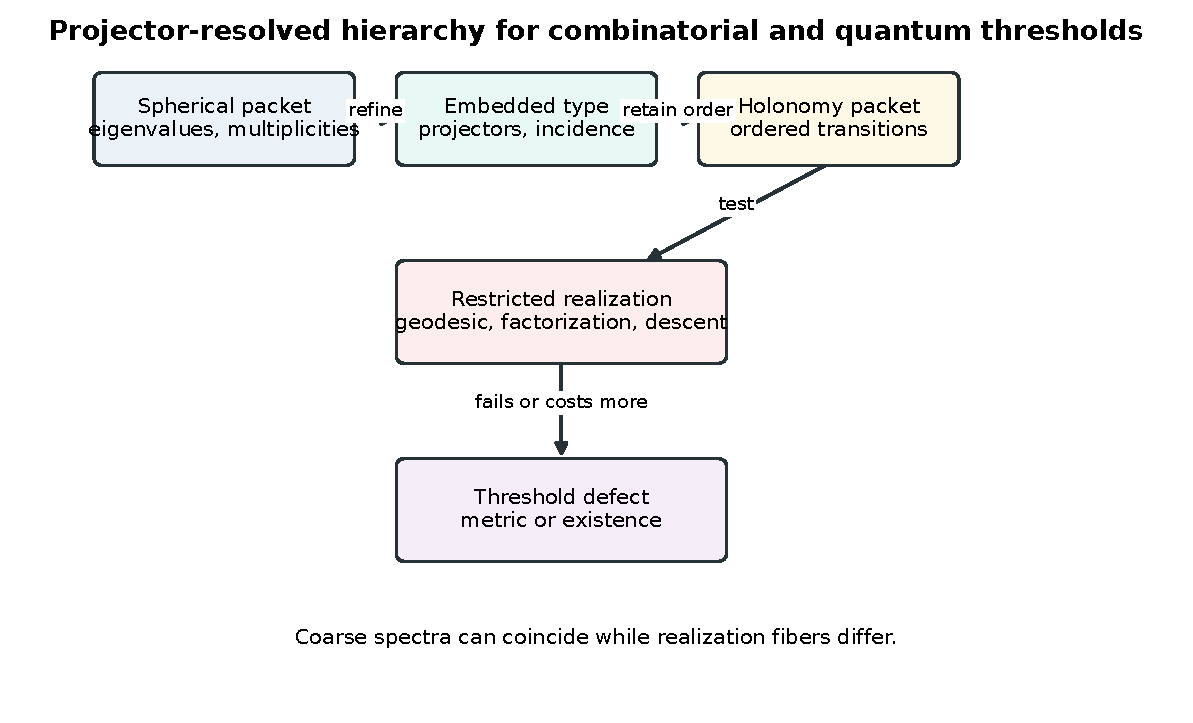
\includegraphics[width=.86\textwidth]{packet_hierarchy.pdf}
\caption{The spectral-to-realization hierarchy.}
\label{fig:packet-hierarchy}
\end{figure}

\begin{boundarybox}
A packet hierarchy organizes evidence.  It does not replace the final lower bound, positivity argument, orthogonality construction, or descent theorem.  Classification and realization remain distinct layers.
\end{boundarybox}

\chapter{Matroidal state geometry, quiver factorizations, and root-system catalysis}\label{ch:matroid-quiver-roots}
\index{matroid}
\index{quiver}
\index{root system}
\index{Chevalley commutator}
\index{pattern group}


\section{Intermediate states as a representable matroid}
A linear circuit visits vectors that satisfy exact dependence relations.  If $\mathcal V$ is the set of all row states appearing during a computation, then $\mathcal V$ determines a representable matroid.  A transvection
\[
u\longmapsto u+a v
\]
creates a three-point projective line
\[
[u],\ [v],\ [u+av].
\]
The ambient circuit chooses a tour through this projective configuration.  A flag-preserving circuit must lift the same dependencies through prescribed pivot positions.

\begin{definition}[Flagged matroid tour]
Let $M$ be a representable matroid with designated initial basis, target basis, and consumer states.  A \emph{flagged tour} is a sequence of basis exchanges or transvections in which the $i$th carrier remains inside a specified filtration layer.  An ambient tour drops this constraint.
\end{definition}
The six-row atom realizes the graphic regular matroid $M(K_4)$.  Its ambient state tour is shorter than every compatible flag lift.  Regularity explains why the same dependence pattern survives every field and, through integer matrices, every nonzero commutative coefficient ring in the stated model.

\section{Matroidal classification problem}
The first general classification problem is:
\begin{quote}
Which regular matroids admit designated carrier and consumer roles for which an ambient tour is shorter than every flag-compatible tour?
\end{quote}
Natural subclasses are graphic, cographic, and network matrices.  Potential invariants include branch width, circuit size, excluded minors, and the number of consumer incidences supported by one projective line.

\begin{conjecturebox}
Minimal field-universal catalytic atoms should be governed by regular matroids, while characteristic-dependent atoms should arise from representable matroids with excluded-characteristic minors.
\end{conjecturebox}
This conjecture is a programmatic guide.  The core paper establishes only the $M(K_4)$ instance.

\section{Dynamic rank-one factorization}
Consider a height-two block shear
\[
E(C)=
\begin{pmatrix}
I_s&0\\
C&I_t
\end{pmatrix}.
\]
A restricted circuit may change source and output bases while transmitting rank-one terms.  Let $P_r\in U_s$ be the source basis before the $r$th transmission and let $Q_{>r}\in U_t$ be the future output basis.  A cross gate contributes
\[
Q_{>r}e_{i_r}e_{j_r}^{T}P_{<r}
\]
to the final block.  Hence
\[
C=
\sum_{r=1}^{c}
Q_{>r}e_{i_r}e_{j_r}^{T}P_{<r},
\]
with closed basis paths
\[
P_{\mathrm{final}}=I_s,
\qquad
Q_{\mathrm{final}}=I_t.
\]

\begin{definition}[Dynamic rank-one cost]
The dynamic rank-one cost of $C$ is the minimum of
\[
\text{source basis motion}
+
\text{output basis motion}
+
\text{number of transmissions}
\]
over such timed decompositions.
\end{definition}
Ordinary rank retains only the number of transmissions after arbitrary bases are given for free.  Circuit complexity charges the closed paths needed to expose and restore those bases.

\section{Quiver gate models}
Let $Q=(Q_0,Q_1)$ be a quiver.  Associate a vector space $V_v$ to every vertex.  Internal gates change bases inside $V_v$, while edge gates transmit low-rank maps along arrows.  A target is a representation of the path algebra or an automorphism of a filtered quiver module.

This generalization includes:
\begin{itemize}
\item block-triangular linear circuits,
\item network coding with reversible local state,
\item layered dataflow architectures,
\item incidence-algebra transformations,
\item tensor networks with reusable bond states.
\end{itemize}

A catalytic excursion can temporarily activate a forbidden arrow or enlarge a vertex space.  The restored target still lies in the original quiver representation class.

\begin{skeletonbox}
A quiver threshold theorem should specify a forbidden-arrow motif, an exact ambient word, a projection-based restricted lower bound, and an amplification operation under quiver substitution.  The unitriangular snapshot family is the linearly ordered one-dimensional-vertex case.
\end{skeletonbox}

\section{Pattern groups and architecture constraints}
For a poset $P$, define the pattern group
\[
U_P(K)
=
\{I+A:A_{ij}=0\text{ unless }j<_P i\}.
\]
When the allowed positions are transitively closed, $U_P$ is a group.  Compare the intrinsic metric generated by $P$-allowed transvections with the metric induced by all transvections.

The first threshold now depends on the forbidden-edge geometry of $P$.  One may ask whether a six-role catalytic motif embeds as a generator-preserving retract.  If it does, the larger architecture inherits a defect.

\begin{proposition}[Retraction inheritance]
Suppose a smaller nested pair $H\le G$ embeds into $H'\le G'$ by homomorphisms preserving the inclusion, the ambient embedding does not increase gate cost, and there is a homomorphic retraction $\pi:H'\to H$ onto the embedded copy.  Require $\ell_H(\pi(s))\le c(s)$ for every restricted generator $s$ of $H'$.  Then every defect in $H\le G$ gives a defect at least as large in $H'\le G'$.
\end{proposition}
The proof projects a restricted word in the larger system and embeds the shorter ambient word from the smaller system.

\section{Root subgroups and Chevalley relations}
Let $G$ be a split reductive group \cite{Carter1972,Humphreys1975} with root system $\Phi$.  Let $\Psi\subseteq\Phi$ be a closed set of allowed roots and let $U_\Psi$ be generated by the root groups $x_\beta(t)$ for $\beta\in\Psi$.  Define
\[
\ell_\Psi(u)
=
\min\{L:u=x_{\beta_L}(t_L)\cdots x_{\beta_1}(t_1),\ \beta_i\in\Psi\},
\]
and let $\ell_\Phi$ permit all roots.

The Chevalley conjugation formula has the schematic form
\[
x_\alpha(a)x_\beta(b)x_\alpha(a)^{-1}
=
x_\beta(b)
\prod_{k>0}
x_{\beta+k\alpha}(c_k a^k b).
\]
A forbidden root $\alpha$ can therefore create several allowed root effects before being removed.

\begin{figure}[ht]
\centering
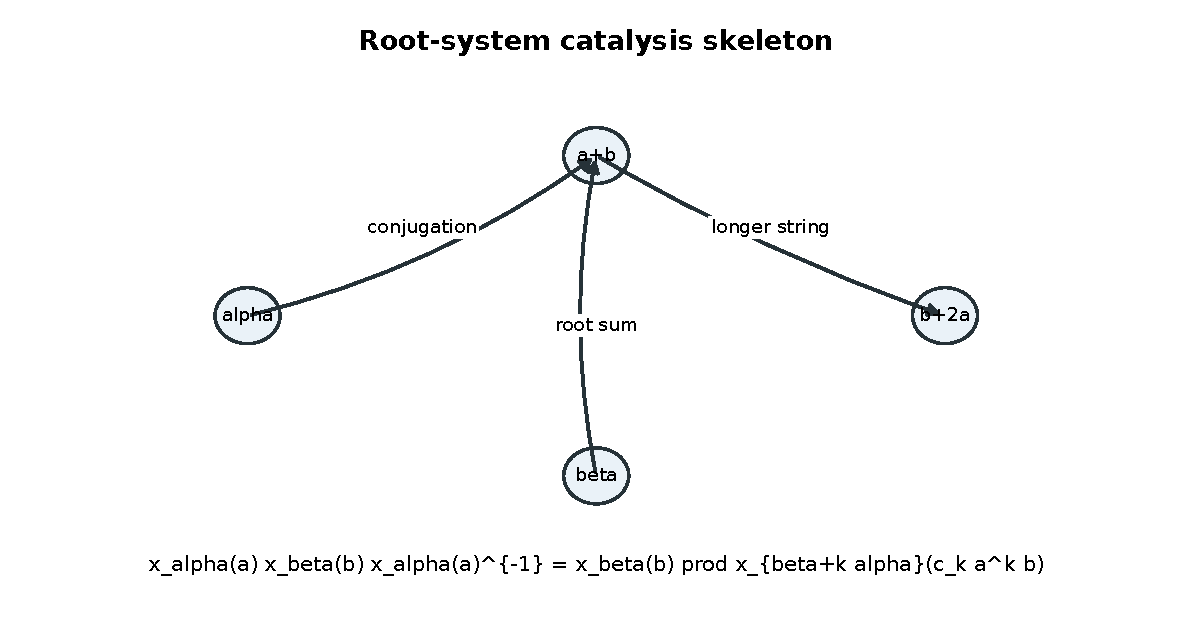
\includegraphics[width=.80\textwidth]{root_catalysis.pdf}
\caption{A root-string template for catalytic generation.  Longer strings may support more gain per opening and closing pair.}
\end{figure}

\section{Type \texorpdfstring{$A$}{A} and beyond}
Row transvections are root-group elements of type $A$.  The established unitriangular atom occurs in $A_5$.  In nonsimply laced systems, root strings can have length greater than two.  This raises the possibility that one ambient root can create multiple restricted effects per consumer.

\begin{conjecture}[Long-root catalytic gain]
There exist gate alphabets in types $B$, $C$, or $G_2$ for which a clean one-catalyst multiplicative distortion exceeds the type-$A$ snapshot limit of $3/2$.
\end{conjecture}
No lower-bound certificate is presently supplied.  The conjecture identifies a concrete reason to test nonsimply laced root systems rather than merely repeating type $A$ computations.

\section{Symplectic root systems and Clifford logic}
The binary Clifford group modulo phases acts through $\Sp(2n,2)$.  A parabolic subgroup stabilizing a Lagrangian is the symplectic analogue of a Borel or flag-preserving circuit class.  Hadamard gates leave this parabolic, while $S$, $\CZ$, and $\CX$ preserve it.  The exact Clifford censuses in \cref{ch:clifford} are therefore a first root-system extension of the linear theory.

\section{Categorical realization defects}
The group framework does not cover measurement, feedforward, postselection, or entangled design objects.  Let
\[
\mathcal C_{\mathrm{res}}
\subseteq
\mathcal C_{\mathrm{amb}}
\]
be monoidal categories with costed generators.  A target morphism can have a finite metric defect or an infinite existence defect.

The categorical viewpoint supports:
\begin{itemize}
\item unitary versus measurement-assisted circuits,
\item product-state versus entangled realizations,
\item clean versus borrowed ancilla categories,
\item symmetry-preserving versus symmetry-breaking channels,
\item exact versus approximate completion.
\end{itemize}
The common invariant is still the cost of a restored target.  What changes is the geometry of the path and the meaning of holonomy.

\section{A general research dichotomy}
The broad program separates into two tasks.
\begin{enumerate}
\item \textbf{Construction:} exhibit an ambient excursion whose repeated consumers produce a cheaper target.
\item \textbf{Certification:} prove that the restricted category cannot share the same obligations as efficiently.
\end{enumerate}
Conjugation identities often solve the first task.  The second is the difficult part and requires model-specific invariants such as interval-tree rank, symplectic flag length, algebraic degree, phase-polynomial rank, covariance constraints, or branch complexity.


\part{Established unitriangular theory}
\chapter{The complete linear core}\label{ch:linear-core}
\index{unitriangular group}\index{CNOT circuit}\index{catalytic escape}\index{tensor amplification}
\begin{boundarybox}
This chapter incorporates the publication-ready unitriangular manuscript.  Its symbolic theorems, exact finite searches, and asymptotic constructions are the proved foundation for the broader gate-set program.  The notation $\ellDown$ and $\ellAll$ specializes $\ellRes$ and $\ellAmb$.
\end{boundarybox}
\section{Introduction}

A CNOT circuit on $n$ labeled wires represents an element of $\GL_n(\F_2)=\SL_n(\F_2)$, and minimizing its gate count is the word-metric problem for transvection generators.  This formulation supports asymptotically efficient synthesis, architecture-aware elimination, computable lower bounds, and exact small-width optimization \cite{SaeediMarkov2013,PatelMarkovHayes2008,JiangEtAl2020,GoubaultEtAl2021,Bataille2022,BuFanJoo2025,ChristensenEtAl2025,WebsterEtAl2025}.  Recent work has also produced stronger explicit lower-bound families and established NP-completeness of exact all-to-all CNOT distance \cite{Jorgensen2026,GongYu2026,AcuavivaEtAl2026}.  The present paper studies a different comparison: the target is lower unitriangular, but the circuit is either required to respect that ordered structure or allowed to leave it temporarily.

Let $R$ be a nonzero commutative ring with identity.  A row transvection is
\[
\tau_{t,s}(a)=I+aE_{t,s},
\qquad t\ne s,
\qquad a\in R\setminus\{0\},
\]
acting by
\[
R_t\longleftarrow R_t+aR_s.
\]
The transvection is \emph{lower directed} when $s<t$.  The lower-directed gates generate $\U_n(R)$.  We compare
\[
\ellDown(A)
 =\min\{\text{number of lower-directed transvections producing }A\}
\]
with
\[
\ellAll(A)
 =\min\{\text{number of arbitrary row transvections producing }A\},
\qquad A\in\U_n(R).
\]
For a field $\F$, the first metric is intrinsic to the unipotent radical and the second is induced from the elementary group $\Egrp_n(\F)=\SL_n(\F)$.

The equality $\ellDown(A)=\ellAll(A)$ is tempting because the target and the obvious Gaussian-elimination paths are lower unitriangular.  It is false.  The failure first occurs at six wires over $\F_2$ and $\F_3$, and it is caused by a reusable temporary carrier rather than by a better ordering of the same lower gates.

\subsection*{Main results}

The first result is entirely analytic and does not require a field.

\begin{theorem}[Universal catalytic atom over rings]\label{thm:universal-atom}
For every nonzero commutative ring $R$ with identity, let
\begin{equation}\label{eq:canonical-C}
C=
\begin{pmatrix}
1&0&0&0&0&0\\
1&1&0&0&0&0\\
0&0&1&0&0&0\\
0&1&1&1&0&0\\
1&1&1&0&1&0\\
1&1&1&0&0&1
\end{pmatrix}
\in\U_6(R).
\end{equation}
Then
\[
\ellDown(C)=7,
\qquad
\ellAll(C)=6.
\]
\end{theorem}

The six-gate ambient circuit uses row $1$ as a dirty workspace.  It first adds row $2$ into row $1$, exports the carrier $e_1+e_2$, changes the carrier to $e_0+e_1+e_2$, exports it twice, and finally removes the temporary $e_2$ component.  No extra wire is introduced.  The workspace is one of the target rows and is restored to its prescribed value.

The next result is computer assisted.  All state spaces are finite, every transition is exact, and the complete source is included in the ancillary archive.

\begin{theorem}[Exact binary threshold and census]\label{thm:binary-census}
Over $\F_2$:
\begin{enumerate}[label=\textup{(\roman*)}]
\item $\ellDown(A)=\ellAll(A)$ for every $A\in\U_n(\F_2)$ when $n\le5$.
\item Among the $2^{15}=32768$ matrices in $\U_6(\F_2)$, exactly twenty satisfy $\ellDown(A)>\ellAll(A)$.
\item Every defective target satisfies
\[
\ellDown(A)=7,
\qquad
\ellAll(A)=6.
\]
No other distance pair is defective.
\end{enumerate}
\end{theorem}

The twenty targets have a uniform combinatorial explanation.

\begin{theorem}[Minimal catalytic classification]\label{thm:motif-classification}
The twenty defective targets in $\U_6(\F_2)$ are exactly the targets generated by a simple one-catalyst word having three cross interactions, one phase interaction, and a nontrivial before/after split across the phase.  The numbers arising from the three possible left/right auxiliary splits are
\[
6,
\qquad
8,
\qquad
6,
\]
for a total of twenty.
\end{theorem}

The field-independent atom and exact ternary search also give the same finite threshold over $\F_3$.

\begin{theorem}[Exact ternary threshold]\label{thm:ternary-threshold}
For $n\le5$ and every $A\in\U_n(\F_3)$,
\[
\ellDown(A)=\ellAll(A).
\]
The matrix $C\in\U_6(\F_3)$ of \cref{eq:canonical-C} has distances $(7,6)$.  Hence six is the first defective dimension over $\F_3$.
\end{theorem}

To pass from the first threshold to arbitrarily large connected examples, we introduce a multiscale rank certificate and a family that exports successive carrier states.

\begin{theorem}[Connected snapshot family]\label{thm:snapshot-family}
Let $u\ge1$, let $1\le v\le u+1$, and choose distinct phases
\[
0\le s_1<\cdots<s_v\le u.
\]
There is a connected target
\[
A(u;s_1,\ldots,s_v)\in\U_{u+v+2}(\F)
\]
with
\[
\ellDown\bigl(A(u;s_1,\ldots,s_v)\bigr)=u+2v
\]
and
\[
\ellAll\bigl(A(u;s_1,\ldots,s_v)\bigr)\le u+v+2.
\]
Hence its certified defect is at least $v-2$.
\end{theorem}

\begin{corollary}[Connected defects in every dimension]\label{cor:connected-gap}
For every field and every $n\ge7$, there is a connected target $A_n\in\U_n(\F)$ satisfying
\[
\ellDown(A_n)-\ellAll(A_n)
\ge
\left\lfloor\frac{n-5}{2}\right\rfloor.
\]
\end{corollary}

The same construction remains effective under stringent restrictions on the ambient resource.

\begin{theorem}[Two forbidden gates and weighted penalties]\label{thm:resource-robustness}
For every field and every $n\ge7$, there is a connected target $A_n\in\U_n(\F)$ such that
\[
\ellBudget{0}(A_n)-\ellBudget{2}(A_n)
\ge
\left\lfloor\frac{n-5}{2}\right\rfloor,
\]
where $\ellBudget{q}$ permits at most $q$ upper-directed gates.  More generally, if lower gates have cost $1$ and upper gates have cost $\lambda>0$, then
\[
\ellDown(A_n)-\ellWeight{\lambda}(A_n)
\ge
\left\lfloor\frac{n-1}{2}\right\rfloor-2\lambda.
\]
Thus no fixed upper-gate budget of two, and no fixed finite upper-gate penalty, suppresses catalytic escape asymptotically.
\end{theorem}

The same paths remain extremely close to the restricted subgroup.  For a matrix $X$ over a field, let $X^+$ be its strict upper part, let $r^+(X)=\rank X^+$, and let $b^+(X)$ be the largest upper displacement $j-i$ with $X_{ij}\ne0$.  If $\ellExc{r}{b}$ denotes the minimum length among circuits satisfying $r^+(X_t)\le r$ and $b^+(X_t)\le b$ at every prefix, then the connected family can be chosen so that
\[
\ellExc{0}{0}(A_n)-\ellExc{1}{1}(A_n)
\ge
\left\lfloor\frac{n-5}{2}\right\rfloor.
\]
Thus a rank-one excursion across one adjacent flag layer can create a linear saving.

At fixed dimension, however, defects occupy thin algebraic strata.

\begin{theorem}[Generic rigidity and defect codimension]\label{thm:generic-rigidity-intro}
Let $K$ be an infinite field and put $N=\binom n2$.  There is a nonempty Zariski-open subset $\Omega_n\subseteq\U_n$ with $\Omega_n(K)\ne\varnothing$ such that
\[
\ellDown(A)=\ellAll(A)=N
\qquad(A\in\Omega_n(K)).
\]
Moreover, after base change to an algebraic closure $\overline K$, for
\[
\mathcal D_{n,\ge d}(\overline K)
=\{A\in\U_n(\overline K):\DeltaDef(A)\ge d\},
\]
one has
\[
\codim_{(\U_n)_{\overline K}}
\overline{\mathcal D_{n,\ge d}(\overline K)}\ge d.
\]
\end{theorem}

\begin{corollary}[Finite-field sparsity]\label{cor:finite-field-sparsity-intro}
Let $N=\binom n2$ and $M=n(n-1)$.  For $1\le d\le N$,
\[
\Prob_{A\in\U_n(\F_q)}[\DeltaDef(A)\ge d]
\le
\min\{1,M^{N-d}q^{-d}\}.
\]
For fixed $n$, a uniformly random target therefore has defect zero with probability $1-O_n(q^{-1})$ as $q\to\infty$.
\end{corollary}

Tensor products produce a stronger asymptotic separation.

\begin{theorem}[Tensor-amplified snapshot family]\label{thm:tensor-main}
Let $A=A(u;s_1,\ldots,s_v)$ have dimension $m=u+v+2$.  For $N=m^r$,
\[
\ellDown(A^{\otimes r})
=r m^{r-1}(u+2v),
\]
while
\[
\ellAll(A^{\otimes r})
\le r m^r.
\]
Consequently,
\[
\ellDown(A^{\otimes r})-\ellAll(A^{\otimes r})
\ge
\frac{v-2}{m\log_2m}N\log_2N.
\]
\end{theorem}

\begin{corollary}[Explicit $n\log n$ distortion]\label{cor:nlogn-gap}
For
\[
D_n(\F)
=
\sup_{A\in\U_n(\F)}
\bigl(\ellDown(A)-\ellAll(A)\bigr),
\]
one has, for every field and every $n$,
\[
D_n(\F)
\ge
\frac{8}{21\log_2 21}n\log_2n
-
\frac{82}{105}n.
\]
The coefficient is attained within the snapshot family by the twenty-one-dimensional seed
\[
A(9;0,1,\ldots,9).
\]
\end{corollary}

\subsection*{Conceptual interpretation}

The ambient circuit is shorter because one forbidden-direction gate creates a carrier that is read by several later gates before it is cleaned.  The saving is therefore a reuse effect.  The relevant object is not an ancillary wire in the usual sense.  It is a temporary excursion from a flag-preserving frame space into the full frame graph.

Over $\F_2$, the carrier states used by the canonical word form six of the seven points of $\operatorname{PG}(2,2)$.  The four projective lines supported on those six points form a Pasch configuration.  The same six vectors represent the graphic matroid $M(K_4)$ over every field; this regular-matroid structure isolates the characteristic-independent core of the atom.  At the spectral level, the distance to a target is the first nonzero coefficient of an endpoint Green kernel.  For $C$, the ambient kernel begins in degree six and the restricted kernel begins in degree seven.

The higher-dimensional families reveal three additional principles.  First, an interval-tree certificate can make the restricted metric exactly additive across scales even when the target is connected.  Second, two forbidden gates can support a linear saving, even if each forbidden gate carries any fixed finite penalty.  Third, tensor products add normalized restricted complexity while ambient complexity remains subadditive.  This converts one local carrier advantage into a superlinear global defect.  Finally, the algebraic-geometric bounds show that these amplifiable atoms are exceptional at fixed dimension: a defect of size $d$ imposes at least $d$ algebraic codimensions.  The resulting picture is one of algebraic rarity coupled with asymptotic amplification.

\subsection*{Scope}

The results concern in-place reversible linear circuits on labeled rows.  They do not by themselves imply a faster general CNOT synthesis algorithm, a lower bound for unrestricted XOR directed acyclic graphs, or a result about integer multiplication.  Their content is a precise comparison between a flag-preserving gate model and the ambient transvection model.

The paper is organized as follows.  \Cref{sec:model} fixes the circuit and metric conventions and gives the Schreier-holonomy interpretation.  \Cref{sec:atom} proves the universal ring-valued atom.  \Cref{sec:catalysis} develops the catalytic normal form and counts the twenty minimal motifs.  \Cref{sec:enumeration} gives the exact binary and ternary enumerations and proves the search procedure complete.  \Cref{sec:geometry-spectrum} gives the projective, regular-matroid, and Green-kernel formulations.  \Cref{sec:higher} develops interval-tree certificates, exact cases through dimension nine, and connected families in every larger dimension.  \Cref{sec:resources} proves bounded, weighted, and microscopic-excursion theorems.  \Cref{sec:rarity} proves generic rigidity, defect-codimension bounds, and finite-field sparsity.  \Cref{sec:amplification} proves block, recursive, and tensor amplification, introduces stable tensor capacity, and derives the $n\log n$ extremal bound.  The appendices provide the exact target list, algorithms, and reproducibility data.

\subsection*{Proof and computation status}
The universal atom, catalytic identities, interval-tree certificates, connected families, resource bounds, algebraic-rarity theorems, amplification results, and stable tensor limit are proved symbolically.  Complete search is used only for the first-threshold censuses, the equality between the twenty computed defects and the twenty analytic motifs, and the exact ambient distances of the selected seven-, eight-, and nine-dimensional targets.  Every computer-assisted statement is paired with a finite-state completeness argument and a reproducible implementation in the supplement.

\section{Circuit model and metric comparison}\label{sec:model}

\subsection{Transvections and row conventions}

Fix a nonzero commutative ring $R$ with identity and an integer $n\ge2$.  Rows and columns are indexed by
\[
0,1,\ldots,n-1.
\]
For $s\ne t$ and $a\in R\setminus\{0\}$, set
\[
\tau_{t,s}(a)=I+aE_{t,s}.
\]
Left multiplication by $\tau_{t,s}(a)$ performs
\[
R_t\longleftarrow R_t+aR_s.
\]
We call $s$ the source and $t$ the target.  A circuit word
\[
w=(\tau_{t_m,s_m}(a_m),\ldots,\tau_{t_1,s_1}(a_1))
\]
produces
\[
[w]=\tau_{t_m,s_m}(a_m)\cdots\tau_{t_1,s_1}(a_1).
\]

Let
\[
S_n^\downarrow(R)
=\{\tau_{t,s}(a):0\le s<t<n,\ a\in R\setminus\{0\}\}
\]
and
\[
S_n^*(R)
=\{\tau_{t,s}(a):0\le s,t<n,\ s\ne t,\ a\in R\setminus\{0\}\}.
\]
Both sets are symmetric because
\[
\tau_{t,s}(a)^{-1}=\tau_{t,s}(-a).
\]
Let
\[
\Egrp_n(R)=\langle S_n^*(R)\rangle.
\]
When $R=\F$ is a field and $n\ge2$, elementary elimination gives
\[
\Egrp_n(\F)=\SL_n(\F).
\]
The ambient metric below is therefore the transvection word metric in $\SL_n(\F)$, viewed inside $\GL_n(\F)$.  When $\F=\F_2$, one has $\SL_n(\F_2)=\GL_n(\F_2)$, every generator is an involution, and it is exactly a CNOT gate under the usual row-action convention.

\begin{lemma}\label{lem:lower-generates}
The set $S_n^\downarrow(R)$ generates $\U_n(R)$.  Every prefix of a lower-directed circuit belongs to $\U_n(R)$.
\end{lemma}

\begin{proof}
A lower-directed transvection is lower unitriangular, and products of lower-unitriangular matrices remain lower unitriangular.  Conversely, ordinary elimination of the strict lower entries, processed in a compatible order, expresses every element of $\U_n(R)$ as a product of lower-directed transvections.
\end{proof}

\begin{definition}[Intrinsic and ambient lengths]\label{def:lengths}
For $A\in\U_n(R)$, define
\[
\ellDown(A)=|A|_{S_n^\downarrow(R)},
\qquad
\ellAll(A)=|A|_{S_n^*(R)}.
\]
The \emph{catalytic defect} is
\[
\DeltaDef(A)=\ellDown(A)-\ellAll(A)\ge0.
\]
\end{definition}

The inequality follows because $S_n^\downarrow(R)\subseteq S_n^*(R)$.  The central question is whether the inclusion can be strict on a lower-unitriangular target.

\subsection{Frame and flag interpretation}

For the geometric interpretation in this subsection, assume $R=\F$ is a field.  An invertible matrix is an ordered basis
\[
(R_0,\ldots,R_{n-1})
\]
of $\F^n$.  A transvection replaces one basis vector by its sum with a nonzero multiple of another.  Let
\[
V_i=\Span(e_0,\ldots,e_i).
\]
A matrix lies in $\U_n(\F)$ exactly when
\[
R_i\in e_i+V_{i-1}
\]
for every $i$.  Thus lower circuits move among frames compatible with the standard complete flag
\[
V_0\subset V_1\subset\cdots\subset V_{n-1}.
\]
An upper-directed gate leaves this fiber of the flag map.  A strict defect means that the flag-compatible frame subgraph is not geodesically convex in the full transvection graph.

\subsection{Schreier holonomy}

Set
\[
G=\Egrp_n(R),
\qquad
H=\U_n(R).
\]
Consider the right Schreier graph on the left cosets $H\backslash G$: a generator $s\in S_n^*(R)$ gives an edge
\[
Hg\longrightarrow Hgs.
\]
A word representing $h\in H$ traces a based loop at the coset $H$.  Its label product is the holonomy $h$.

\begin{proposition}[Holonomy-compression interpretation]\label{prop:schreier-holonomy}
For $h\in H$, the ambient length $\ellAll(h)$ is the least length of a labeled based loop in $H\backslash G$ with holonomy $h$.  The restricted length $\ellDown(h)$ is the least length among such words whose every prefix remains in $H$.  Consequently,
\[
\DeltaDef(h)
=
\text{intrinsic flag-preserving cost}
-
\text{shortest ambient holonomy-loop cost}.
\]
\end{proposition}

\begin{proof}
A word $w=s_1\cdots s_k$ ends at the coset $Hw$.  It is a based loop exactly when $w\in H$, and its label product is then the represented element of $H$.  Minimizing over all transvection words representing $h$ gives $\ellAll(h)$.  Requiring every generator to be lower directed keeps every prefix in $H$ and gives $\ellDown(h)$.
\end{proof}

A catalytic shortcut is therefore a nonconstant quotient excursion whose accumulated holonomy is more expensive to produce inside the base fiber.

\subsection{Two elementary counting lemmas}

The proofs of the universal atom use only target counts and pivot support.

\begin{lemma}[Target count]\label{lem:target-count}
Suppose a circuit starts at the identity and finishes at $A$.
\begin{enumerate}[label=\textup{(\roman*)}]
\item If row $i$ of $A$ differs from $e_i$, then row $i$ is targeted at least once.
\item If row $i$ of $A$ equals $e_i$ and is targeted, then it is targeted at least twice.
\end{enumerate}
\end{lemma}

\begin{proof}
A row changes only when it is targeted.  Every row of an invertible matrix over $R$ is unimodular.  If $aR_s=0$ for such a row, then multiplying a unimodular relation for $R_s$ by $a$ gives $a=0$.  Hence a gate with nonzero coefficient changes its target by a nonzero vector, so one targeting cannot leave that row equal to its initial value.
\end{proof}

\begin{lemma}[One-target source condition]\label{lem:one-target-source}
Let $W\le R^n$.  Suppose row $t$ starts at $e_t$, is targeted exactly once, and finishes at
\[
e_t+w,
\qquad w\in W,
\]
where at least one coordinate of $w$ is a unit of $R$.  At the moment of its unique targeting, the gate coefficient is a unit and the source row is a unit multiple of $w$.
\end{lemma}

\begin{proof}
If the unique gate is $R_t\leftarrow R_t+aR_s$, then $aR_s=w$.  Choose a coordinate $j$ for which $w_j$ is a unit.  Since $a(R_s)_j=w_j$, the factor $a$ is a unit in the commutative ring $R$.  Hence $R_s=a^{-1}w$.
\end{proof}

The second lemma is especially restrictive when $W$ is a low-dimensional source space and output rows carry unique pivot coordinates outside $W$.

\section{The universal six-row atom}\label{sec:atom}

Let $R$ be a nonzero commutative ring with identity, and let
\[
v=e_1+e_2,
\qquad
w=e_0+e_1+e_2,
\qquad
W=\Span(e_0,e_1,e_2).
\]
The target $C$ of \cref{eq:canonical-C} has rows
\begin{align*}
R_0&=e_0,
& R_1&=e_1+e_0,
& R_2&=e_2,\\
R_3&=e_3+v,
& R_4&=e_4+w,
& R_5&=e_5+w.
\end{align*}

\begin{figure}[t]
\centering
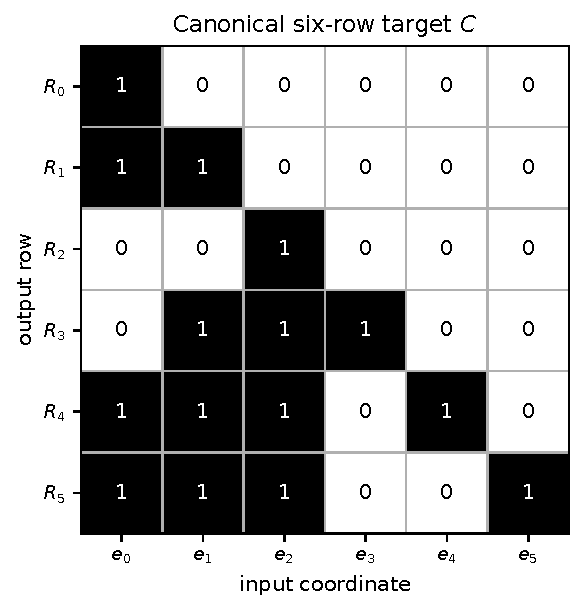
\includegraphics[width=.56\linewidth]{canonical_matrix.pdf}
\caption{The canonical target $C$.  Black cells are nonzero.  Rows $0$ and $2$ are restored exactly, while rows $3,4,5$ require two distinct additions $v$ and $w$ from the source space $W$.}
\label{fig:canonical-matrix}
\end{figure}

\subsection{A six-gate ambient word}

\begin{proposition}\label{prop:ambient-upper}
For every nonzero commutative ring $R$ with identity,
\[
\ellAll(C)\le6.
\]
\end{proposition}

\begin{proof}
Apply the following six gates:
\begin{align}
R_1&\leftarrow R_1+R_2,\label{gate:a1}\\
R_3&\leftarrow R_3+R_1,\label{gate:a2}\\
R_1&\leftarrow R_1+R_0,\label{gate:a3}\\
R_4&\leftarrow R_4+R_1,\label{gate:a4}\\
R_5&\leftarrow R_5+R_1,\label{gate:a5}\\
R_1&\leftarrow R_1-R_2.\label{gate:a6}
\end{align}
After \cref{gate:a1}, row $1$ contains $v$.  Gate \cref{gate:a2} copies $v$ to row $3$.  Gate \cref{gate:a3} changes the carrier to $w$, which is copied to rows $4$ and $5$ by \cref{gate:a4,gate:a5}.  Gate \cref{gate:a6} removes the temporary $e_2$ component, leaving $e_1+e_0$.  Every row now agrees with $C$.
\end{proof}

\begin{figure}[t]
\centering
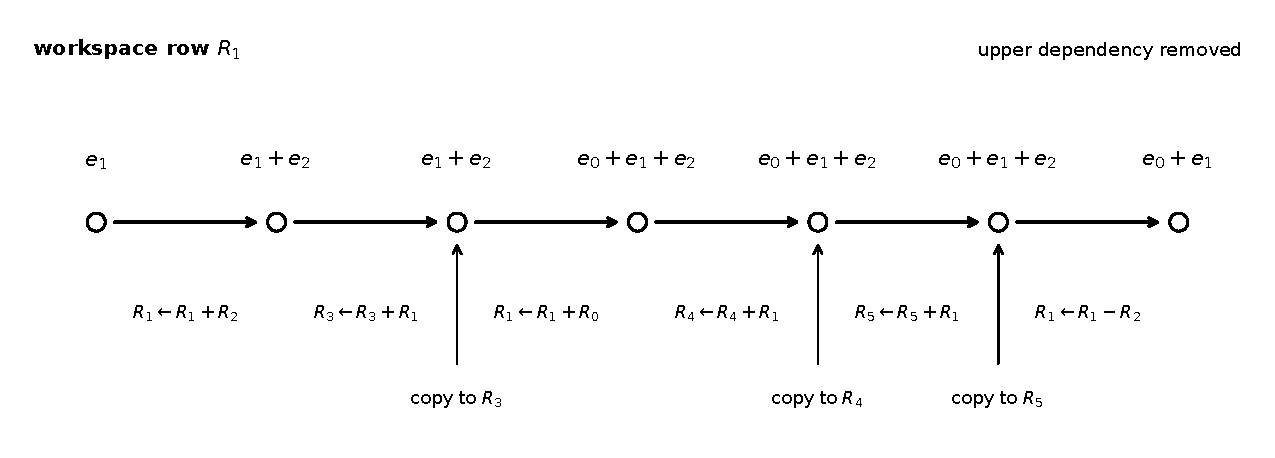
\includegraphics[width=.98\linewidth]{carrier_timeline.pdf}
\caption{Carrier timeline for the six-gate ambient word.  The two upper-directed operations are the opening and closing gates on row $1$.  The state $e_1+e_2$ is exported once and $e_0+e_1+e_2$ is exported twice.}
\label{fig:carrier-timeline}
\end{figure}

\subsection{A seven-gate lower word}

\begin{proposition}\label{prop:lower-upper}
For every nonzero commutative ring $R$ with identity,
\[
\ellDown(C)\le7.
\]
\end{proposition}

\begin{proof}
The lower-directed word
\begin{align*}
R_1&\leftarrow R_1+R_0,\\
R_2&\leftarrow R_2+R_1,\\
R_3&\leftarrow R_3-R_0,\\
R_3&\leftarrow R_3+R_2,\\
R_4&\leftarrow R_4+R_2,\\
R_5&\leftarrow R_5+R_2,\\
R_2&\leftarrow R_2-R_1
\end{align*}
produces $C$.  After the first two gates, row $2$ contains $w$.  Rows $4$ and $5$ copy that state.  The two gates on row $3$ cancel the unwanted $e_0$ and leave $v$.  The final gate restores row $2$.
\end{proof}

\subsection{Restricted lower bound}

\begin{proposition}\label{prop:lower-lower-bound}
For every nonzero commutative ring $R$ with identity,
\[
\ellDown(C)\ge7.
\]
\end{proposition}

\begin{proof}
Rows $1,3,4,5$ differ from their initial values, so they must each be targeted.  Assume for contradiction that a lower-directed word of length at most six produces $C$.

First suppose row $2$ is never targeted.  Row $0$ remains $e_0$, row $2$ remains $e_2$, and every state ever assumed by row $1$ lies in $\Span(e_0,e_1)$ because the only possible source below row $1$ is row $0$.  Every output row retains coefficient $1$ on its own pivot coordinate in a lower-directed circuit, so no output row can lie in $W$.  Hence no available source row is a unit multiple of either
\[
v=e_1+e_2
\quad\text{or}\quad
w=e_0+e_1+e_2.
\]
By \cref{lem:one-target-source}, each of rows $3,4,5$ must be targeted at least twice.  Together with the required targeting of row $1$, this gives at least seven gates.

Now suppose row $2$ is targeted.  Since its final value is $e_2$, \cref{lem:target-count} forces at least two targetings of row $2$.  A six-gate word must therefore target row $2$ exactly twice and each of rows $1,3,4,5$ exactly once.  Each output row $3,4,5$ must receive its complete addition in its unique targeting.  Row $0$ cannot supply $v$ or $w$, and row $1$ never contains an $e_2$ component.  Therefore row $2$ must supply all three outputs, up to unit scaling.  But two targetings of row $2$ expose at most one noninitial intermediate state before row $2$ returns to $e_2$, while the outputs require both distinct states $v$ and $w$.  This is impossible.
\end{proof}

\subsection{Ambient lower bound}

\begin{proposition}\label{prop:ambient-lower-bound}
For every nonzero commutative ring $R$ with identity,
\[
\ellAll(C)\ge6.
\]
\end{proposition}

\begin{proof}
Assume that an ambient word of length at most five produces $C$.  Rows $1,3,4,5$ must each be targeted.  Rows $0$ and $2$ are unchanged.  If either were targeted, it would require at least two targetings, giving at least six gates in total.  Thus rows $0$ and $2$ are never targeted.  If all four changed rows are targeted once, each has only its initial and final state.  No such source is a unit multiple of $v=e_1+e_2$ or $w=e_0+e_1+e_2$, so the output rows cannot be completed.  In the only remaining case, exactly one of rows $1,3,4,5$ is targeted twice and the other three are targeted once.

Project the rows to the quotient module $R^6/W$.  Rows $0,1,2$ have zero image, while rows $3,4,5$ begin and end at the three distinct quotient basis vectors of the free quotient module.  An output row targeted exactly once must therefore use a source lying in $W$, by \cref{lem:one-target-source}.

Suppose first that row $1$ is the twice-targeted row.  The three output rows are each targeted once.  Rows $0$ and $2$ supply only scalar multiples of $e_0$ and $e_2$.  Row $1$ begins at $e_1$, has one intermediate state, and ends at $e_1+e_0$.  Thus at most one of the two required unit-multiple classes of $v$ and $w$ can appear as an available source.  The three outputs require both, a contradiction.

Suppose instead that an output row, say row $r\in\{3,4,5\}$, is targeted twice.  The other two outputs and row $1$ are targeted once.  We claim that row $r$ cannot lie in $W$ between its two targetings.  To cancel its unique quotient pivot $e_r$ at the first targeting, the source would already have to contain an $e_r$ component.  Before row $r$ is first targeted, the only way another row can acquire such a component is to be targeted using row $r$ as source.  That other row is targeted only once and would then retain an unwanted $e_r$ component in its final value.  Therefore row $r$ never becomes a $W$-valued carrier.  The only $W$-valued source states are rows $0$ and $2$ and the two states of singly targeted row $1$, namely its initial and final states.  None supplies both $v$ and $w$.  The two singly targeted outputs cannot be completed, again a contradiction.
\end{proof}

\begin{proof}[Proof of \cref{thm:universal-atom}]
Combine \cref{prop:ambient-upper,prop:lower-upper,prop:lower-lower-bound,prop:ambient-lower-bound}.
\end{proof}

\begin{remark}
The proof uses only unimodular rows, unit coordinates, and pivot support.  It does not use division or a characteristic assumption.  In characteristic two the closing subtraction equals addition.
\end{remark}

\begin{corollary}[Failure of geodesic convexity]\label{cor:nonconvex}
For every field $\F$ and every $n\ge6$, the lower-unitriangular frame subgraph is not geodesically convex in the transvection Cayley graph of $\Egrp_n(\F)=\SL_n(\F)$.
\end{corollary}

\begin{proof}
Embed $C$ as $C\oplus I_{n-6}$.  A six-gate ambient word acts on the first six rows.  In a lower-directed circuit, rows with index at least six cannot be used as sources for targets among the first six rows, so the restricted lower bound of seven persists.
\end{proof}

For the remainder of the paper, unless explicitly stated otherwise, the coefficient domain is a field $\F$.

\section{Catalytic normal forms and the six-role threshold}\label{sec:catalysis}

The universal atom is one instance of a root-conjugation mechanism.  This section isolates that mechanism and explains the count twenty.

\subsection{Root conjugation identities}

Let $p<q<y$ and $x<p<q$.  Direct multiplication gives
\begin{equation}\label{eq:read-conjugation}
\tau_{p,q}(-a)\,\tau_{y,p}(b)\,\tau_{p,q}(a)
=
\tau_{y,p}(b)\,\tau_{y,q}(ab),
\end{equation}
and
\begin{equation}\label{eq:update-conjugation}
\tau_{p,q}(-a)\,\tau_{q,x}(b)\,\tau_{p,q}(a)
=
\tau_{q,x}(b)\,\tau_{p,x}(-ab).
\end{equation}
A single forbidden upper transvection can therefore turn one lower interaction into two lower effects.  Interactions of the forms $x\to p$ and $q\to y$ commute through the excursion without duplication.  We call the duplicated interactions \emph{cross interactions} and the unduplicated interactions \emph{phase interactions}.

\begin{definition}[Simple one-catalyst word]\label{def:simple-catalyst}
A simple one-catalyst word has the form
\[
\tau_{p,q}(-a)\,h_m\cdots h_1\,\tau_{p,q}(a),
\qquad p<q,
\]
where every $h_i$ is lower directed and is one of
\[
\tau_{q,x}(b),\quad \tau_{p,x}(b),\quad
\tau_{y,p}(b),\quad \tau_{y,q}(b)
\]
with $x<p<q<y$.  Auxiliary rows are distinct unless stated otherwise.
\end{definition}

The circuit is read from right to left in the matrix product and from left to right as a gate list.  The opening and closing operations temporarily place the $q$ component in row $p$.

\begin{proposition}[Cross-interaction accounting]\label{prop:cross-accounting}
Let a simple one-catalyst word have $m$ middle interactions, of which $c$ are cross interactions.  Its target admits a lower-directed realization of length at most
\[
m+c.
\]
Consequently, if the ambient word of length $m+2$ is strictly shorter than every lower word, then
\[
c\ge3.
\]
\end{proposition}

\begin{proof}
Conjugate each middle generator using \cref{eq:read-conjugation,eq:update-conjugation}.  A phase interaction remains one lower transvection, while a cross interaction becomes a product of two lower transvections.  This gives length at most $m+c$.  If $c\le2$, then $m+c\le m+2$, so the ambient excursion cannot be strictly better.
\end{proof}

Three consumers are therefore the first possible point at which the cost two of opening and closing can be amortized.

\subsection{Why an all-cross word is insufficient}

Within the distinct-leaf normal form, cross count alone is not enough.

\begin{lemma}[All-cross mirror]\label{lem:all-cross-mirror}
Suppose a simple one-catalyst word contains only cross interactions, with left inputs $X$ and right outputs $Y$.  Then its target has a lower-directed realization with the same number of gates.
\end{lemma}

\begin{proof}
Write the opening coefficient as $a\in\F^\times$, the left-update coefficients as $b_x$, and the right-read coefficients as $c_y$.  Since the all-cross middle gates commute past one another, the ambient gate list may be written
\[
R_p\leftarrow R_p+aR_q;
\quad
[R_q\leftarrow R_q+b_xR_x]_{x\in X};
\quad
[R_y\leftarrow R_y+c_yR_p]_{y\in Y};
\quad
R_p\leftarrow R_p-aR_q.
\]
Put $B=\sum_{x\in X}b_xe_x$.  Its final nontrivial rows are
\[
R_p=e_p-aB,
\qquad
R_q=e_q+B,
\qquad
R_y=e_y+c_ye_p+ac_ye_q
\quad(y\in Y).
\]
The following lower-directed gate list produces the same rows:
\[
R_q\leftarrow R_q+a^{-1}R_p;
\quad
[R_y\leftarrow R_y+ac_yR_q]_{y\in Y};
\quad
[R_p\leftarrow R_p-ab_xR_x]_{x\in X};
\quad
R_q\leftarrow R_q-a^{-1}R_p.
\]
Indeed, after the first gate $R_q=e_q+a^{-1}e_p$, so the output gates create exactly $c_ye_p+ac_ye_q$.  The source updates then leave $R_p=e_p-aB$, and the final gate changes $R_q$ to $e_q+B$.  Both words have $|X|+|Y|+2$ gates.
\end{proof}

Thus a minimal strict shortcut needs both positive catalytic excess and a phase switch that makes temporal order matter.

\begin{proposition}[Six-role threshold in the simple model]\label{prop:six-role}
A strict shortcut in the distinct-leaf simple one-catalyst model requires at least six row roles:
\[
2\text{ catalyst rows}
+
3\text{ cross interactions}
+
1\text{ phase interaction}.
\]
The bound is attained by the matrix $C$.
\end{proposition}

\begin{proof}
By \cref{prop:cross-accounting}, at least three cross interactions are required.  By \cref{lem:all-cross-mirror}, at least one phase interaction is required.  With distinct leaves these use four auxiliary rows in addition to the two catalyst rows.  The word of \cref{prop:ambient-upper} has exactly this form.
\end{proof}

\begin{figure}[t]
\centering
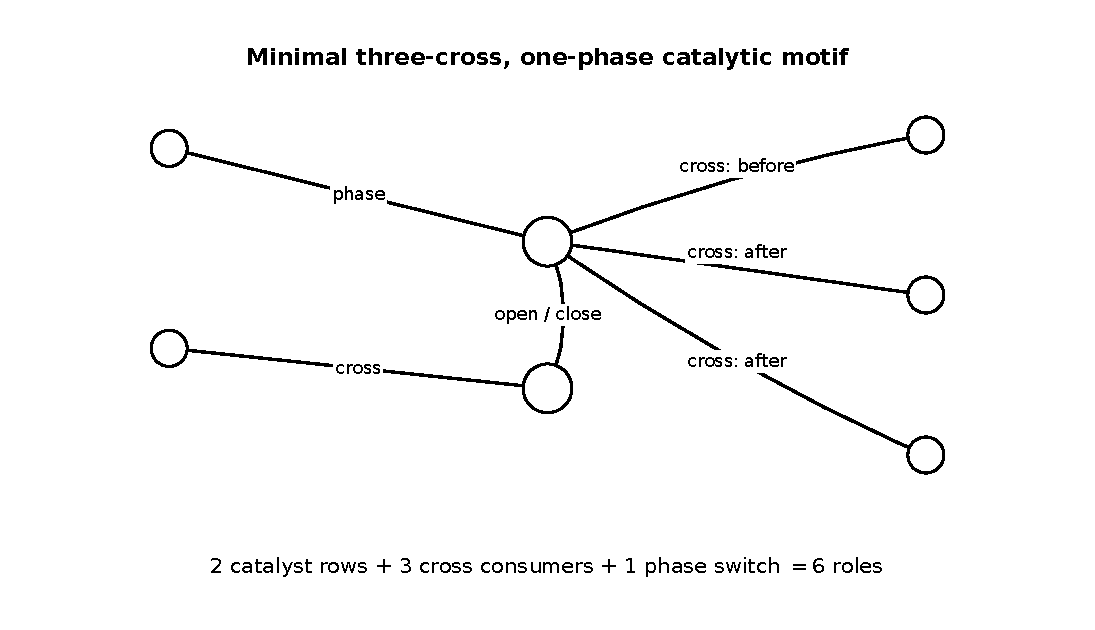
\includegraphics[width=.82\linewidth]{catalytic_motif.pdf}
\caption{The minimal one-catalyst motif.  Cross interactions reuse the opened carrier.  The phase gate separates consumers that observe two different carrier states and prevents the all-cross mirror.}
\label{fig:catalytic-motif}
\end{figure}

\subsection{Enumeration of the minimal motifs}

Fix six ordered rows.  The catalyst pair must be adjacent in a minimal six-role word.  Write
\[
p<q=p+1,
\]
let $L$ be the set of rows left of $p$, and let $R$ be the set of rows right of $q$.  Then
\[
|L|+|R|=4,
\qquad
|L|,|R|>0.
\]
There are two orientations.

\paragraph{Left phase.}
Choose a phase leaf $x\in L$.  The remaining $|L|-1$ left leaves interact by $u\to q$.  Every right leaf is a cross read $p\to y$.  To make the phase effective, the right leaves are divided into a nonempty set read before $x\to p$ and a nonempty set read after it.  The number of targets is
\[
|L|\bigl(2^{|R|}-2\bigr).
\]

\paragraph{Right phase.}
Choose a phase leaf $y\in R$.  Every other right leaf is a cross read.  The left updates into $q$ are divided nontrivially before and after the phase gate $q\to y$.  The number is
\[
|R|\bigl(2^{|L|}-2\bigr).
\]

\begin{proposition}[Motif count]\label{prop:motif-count}
For a split $(L,R)=(|L|,|R|)$ with $L+R=4$, the number of minimal phase-separated targets is
\[
N_{L,R}
=L(2^R-2)+R(2^L-2).
\]
For the three possible splits,
\[
N_{1,3}=6,
\qquad
N_{2,2}=8,
\qquad
N_{3,1}=6.
\]
Hence there are twenty targets.
\end{proposition}

\begin{proof}
The preceding left-phase and right-phase constructions are disjoint because the phase row lies on opposite sides of the catalyst.  Within each orientation, the final support records the phase leaf and the before/after subset, so distinct choices give distinct targets.  Summing gives the formula and the stated values.
\end{proof}

\begin{figure}[t]
\centering
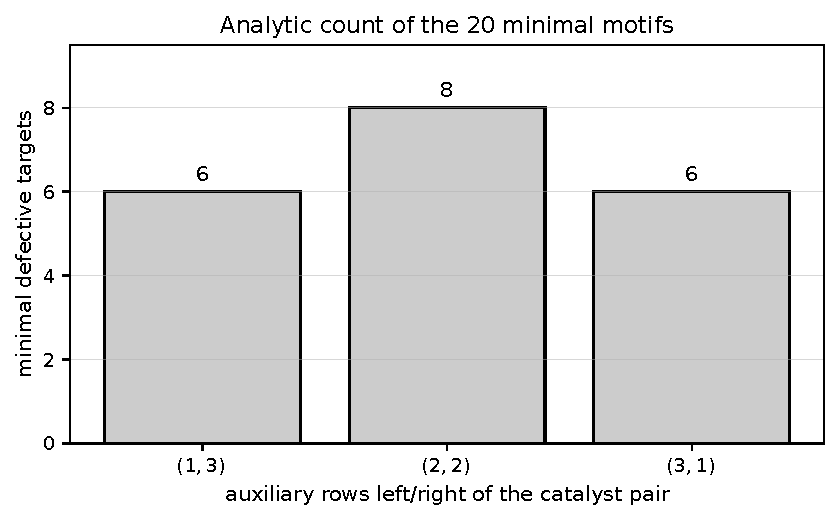
\includegraphics[width=.70\linewidth]{motif_count.pdf}
\caption{The analytic count of the twenty minimal catalytic targets.}
\label{fig:motif-count}
\end{figure}

Every target counted by \cref{prop:motif-count} has an explicit six-gate ambient word and a seven-gate lower word obtained by eliminating the three cross interactions.  The nontrivial statement is that there are no other defects in dimension six and that none of these targets has a lower word of length six.  That is the exact classification established in \cref{sec:enumeration}.

\section{Exact finite enumeration}\label{sec:enumeration}

This section describes the computer-assisted part of the paper.  The computations use integer encodings only.  No floating-point decisions occur.

\subsection{Restricted breadth-first search}

Over $\F_2$, an element of $\U_n(\F_2)$ is determined by its $n(n-1)/2$ strict lower entries.  For $n=6$ there are $2^{15}=32768$ states.  Breadth-first search from the identity using the fifteen lower transvections gives every restricted distance and the restricted diameter.

For $n=6$, the restricted diameter is eight.  Therefore every lower-unitriangular target has ambient distance at most eight.  This makes a radius-four meet-in-the-middle search complete.

\subsection{Ambient radius-four ball and right-coset pairing}

Let
\[
B_4=\{g\in\GL_6(\F_2):\ellAll(g)\le4\}.
\]
Exact breadth-first search gives
\[
|B_4|=110626.
\]
Group $B_4$ by right cosets of $\U_6(\F_2)$.  If $a,b$ lie in the same right coset, then
\[
b^{-1}a\in\U_6(\F_2),
\]
and
\[
\ellAll(b^{-1}a)\le\ellAll(b)+\ellAll(a)\le8.
\]
The implementation uses a canonical right-coset key obtained by reducing matrix columns from right to left.  Right multiplication by a lower-unitriangular matrix changes column $j$ only by a combination of columns with larger index, so this reduction is constant on right cosets and separates them.

\begin{lemma}[Meet-in-the-middle completeness]\label{lem:mitm-complete}
For every $u\in\U_6(\F_2)$,
\[
\ellAll(u)
=
\min\{\ellAll(a)+\ellAll(b):a,b\in B_4,\ b^{-1}a=u\}.
\]
\end{lemma}

\begin{proof}
Every pair on the right gives a word for $u$, so the right-hand side is at least $\ellAll(u)$.  Conversely, $\ellAll(u)\le8$.  Take a shortest path from the identity to $u$ and split it at a midpoint.  The prefix endpoint $a$ has distance at most four.  The inverse of the remaining suffix is an element $b$ of distance at most four, and $u=b^{-1}a$.  Hence the minimum is at most $\ellAll(u)$.
\end{proof}

The radius-four ball splits into $6948$ right-coset buckets.  The largest bucket has $3775$ elements.  The computation checks $45178326$ ordered pairs and recovers an ambient distance for every one of the $32768$ targets.

\subsection{The exact binary census}

\begin{table}[t]
\centering
\caption{Complete distance distribution in $\U_6(\F_2)$.}
\label{tab:census}
\begin{tabular}{@{}rrr@{}}
\toprule
$\ellDown$ & $\ellAll$ & number of targets\\
\midrule
0&0&1\\
1&1&15\\
2&2&125\\
3&3&720\\
4&4&2914\\
5&5&7851\\
6&6&12656\\
7&6&20\\
7&7&7926\\
8&8&540\\
\bottomrule
\end{tabular}
\end{table}

\begin{figure}[t]
\centering
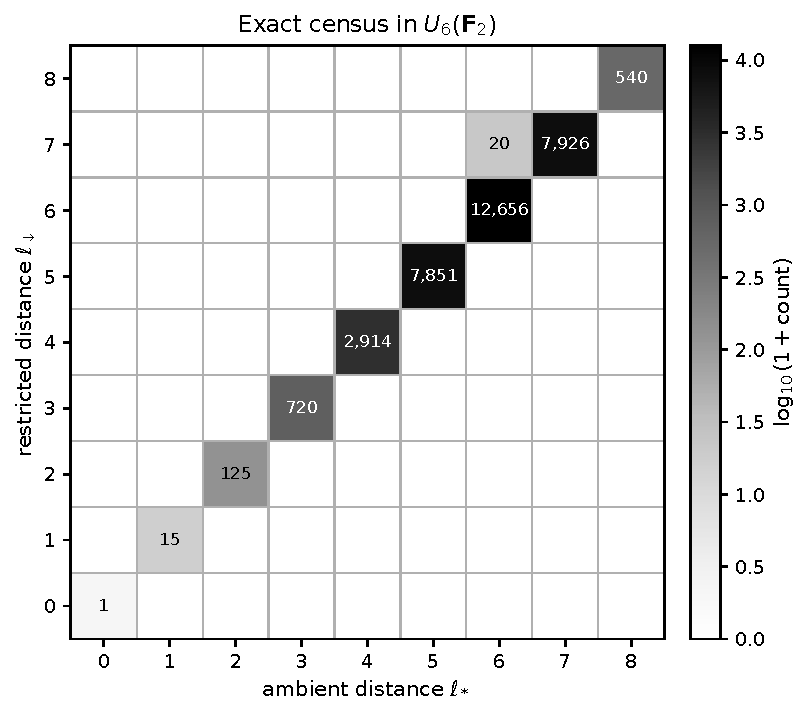
\includegraphics[width=.72\linewidth]{distance_census.pdf}
\caption{Complete binary dimension-six census.  The only off-diagonal cell contains the twenty targets with distance pair $(7,6)$.}
\label{fig:distance-census}
\end{figure}

\begin{proof}[Proof of \cref{thm:binary-census}]
For $n=2,3,4,5$, complete restricted breadth-first search and complete ambient meet-in-the-middle search return zero defects.  The state counts are respectively $2,8,64,1024$.  For $n=6$, \cref{lem:mitm-complete} proves that the ambient calculation is exhaustive.  The resulting distribution is \cref{tab:census}; its counts sum to $32768$, no target is missing, and the only strict pair is $(7,6)$ with multiplicity twenty.
\end{proof}

\begin{proof}[Proof of \cref{thm:motif-classification}]
The analytic generator of \cref{prop:motif-count} produces twenty distinct targets without reference to the distance census.  Exact set comparison shows that these twenty targets are precisely the twenty off-diagonal targets in \cref{tab:census}.  Each therefore has distances $(7,6)$, and no other dimension-six target is defective.
\end{proof}

\subsection{Ternary and additional field checks}

For $\F_3$, every nonzero scaled transvection is included.  Complete searches give the data in \cref{tab:small-fields}.

\begin{table}[t]
\centering
\caption{Complete no-defect computations below dimension six.}
\label{tab:small-fields}
\begin{tabular}{@{}crrr@{}}
\toprule
field & $n$ & $|\U_n(\F)|$ & restricted diameter\\
\midrule
$\F_2$&2&2&1\\
$\F_2$&3&8&2\\
$\F_2$&4&64&4\\
$\F_2$&5&1024&6\\
\addlinespace
$\F_3$&2&3&1\\
$\F_3$&3&27&3\\
$\F_3$&4&729&5\\
$\F_3$&5&59049&7\\
\bottomrule
\end{tabular}
\end{table}

The $n=5$ ternary computation uses radius-three and radius-four balls, checks $38415205$ right-coset pairs, and recovers all $59049$ targets.  It finds no defect.  The field-independent \cref{thm:universal-atom} supplies a defect at $n=6$, proving \cref{thm:ternary-threshold}.  Separate exact searches over $\F_3$ and $\F_5$ verify the distances of the canonical atom directly.  The $\F_5$ calculation is an audit of the atom, not a complete threshold computation below dimension six.

\subsection{Verification status}

The analytic proofs of \cref{thm:universal-atom,cor:linear-gap} do not depend on computation.  The claims in \cref{thm:binary-census,thm:motif-classification,thm:ternary-threshold} depend on exact finite enumeration.  The source archive contains:
\begin{itemize}
\item the C++ programs for every breadth-first and meet-in-the-middle search;
\item the Python program that independently generates the twenty motifs and compares sets;
\item symbolic checks for the bounded-resource formulas and the totally unimodular $M(K_4)$ representation;
\item exact stdout files and JSON packet data;
\item SHA-256 checksums;
\item build and reproduction commands.
\end{itemize}
The programs were rebuilt from source and rerun independently when this manuscript was assembled; the outputs matched byte for byte.

\section{Projective, matroidal, and spectral structure}\label{sec:geometry-spectrum}

\subsection{The flagged Pasch packet}

Over $\F_2$, write
\[
x=e_0,
\qquad
p=e_1,
\qquad
q=e_2.
\]
The canonical ambient word uses the six nonzero vectors
\[
x,
\quad p,
\quad q,
\quad p+q,
\quad p+q+x,
\quad p+x
\]
inside $\Span(x,p,q)\cong\F_2^3$.  The only missing nonzero vector is $x+q$.

In $\operatorname{PG}(2,2)$, three distinct points form a line exactly when their vector representatives sum to zero.  The six points support the four lines
\[
\{x,p,x+p\},
\quad
\{x,p+q,x+p+q\},
\quad
\{p,q,p+q\},
\quad
\{x+p,q,x+p+q\}.
\]
Every point lies on exactly two of these lines.  This is the Pasch configuration, equivalently the Fano plane with one point and its three incident lines removed from the full incidence structure.

\begin{figure}[t]
\centering
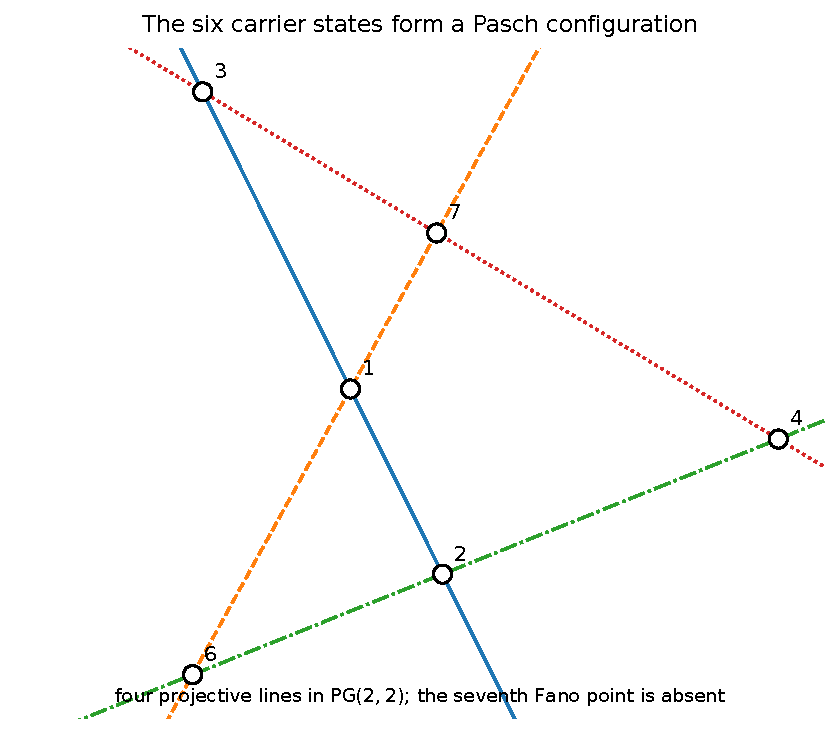
\includegraphics[width=.65\linewidth]{pasch_configuration.pdf}
\caption{A real drawing of the four-line Pasch incidence structure.  The labels are the binary point encodings $1,2,3,4,6,7$; point $5$ is the missing Fano point.}
\label{fig:pasch}
\end{figure}

The configuration is flagged because the rows have fixed roles.  Points $x$ and $q$ are stationary sources, $p$ is the carrier, and the remaining points occur as carrier states.  Forgetting those roles loses the circuit ordering information.

\subsection{The regular matroid \texorpdfstring{$M(K_4)$}{M(K4)}}

The six carrier states admit a field-independent representation.  In the ordered basis $(x,p,q)$, place them as the columns of
\begin{equation}\label{eq:k4-matrix}
B=
\begin{pmatrix}
1&0&0&1&0&1\\
0&1&0&1&1&1\\
0&0&1&0&1&1
\end{pmatrix},
\end{equation}
corresponding respectively to
\[
x,
\quad p,
\quad q,
\quad x+p,
\quad p+q,
\quad x+p+q.
\]

\begin{proposition}[Regular-matroid core]\label{prop:regular-matroid}
Every square minor of $B$ belongs to $\{0,\pm1\}$, so $B$ is totally unimodular.  Hence the column-dependence matroid is the same over every field.  Under the edge labeling
\[
\begin{array}{c|cccccc}
\text{state}&p&x&x+p&p+q&q&x+p+q\\
\hline
K_4\text{ edge}&12&13&23&14&24&34,
\end{array}
\]
it is the graphic matroid $M(K_4)$.
\end{proposition}

\begin{proof}
A direct calculation of all square minors of $B$ gives only $0$, $1$, and $-1$.  Thus every subdeterminant has characteristic-independent vanishing, and a column set is independent over one field exactly when it is independent over every field.  The four minimal dependent triples are
\[
\{x,p,x+p\},
\quad
\{p,q,p+q\},
\quad
\{x,p+q,x+p+q\},
\quad
\{q,x+p,x+p+q\}.
\]
Under the displayed edge labeling, these are precisely the four triangular cycles of $K_4$.  They determine the rank-three cycle matroid $M(K_4)$, which is regular because it has a totally unimodular representation; see, for example, \cite{Oxley2011}.
\end{proof}

\begin{figure}[t]
\centering
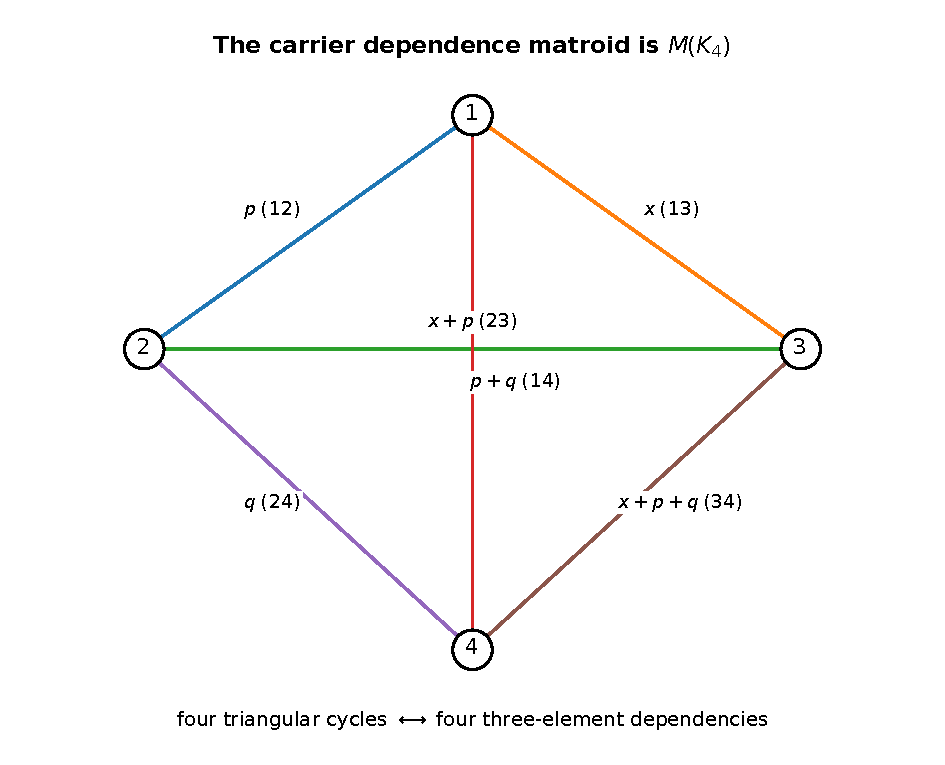
\includegraphics[width=.72\linewidth]{regular_matroid_k4.pdf}
\caption{The six carrier states as the edges of $K_4$.  Each triangular cycle is one of the four three-element dependencies in the Pasch configuration.  The resulting regular matroid is representable over every field.}
\label{fig:k4-matroid}
\end{figure}

The field-independent circuit theorem is stronger than matroid representability alone, because it also depends on the ordering and the designated carrier role.  Nevertheless, \cref{prop:regular-matroid} explains why the local dependence pattern survives unchanged in every characteristic.

\subsection{Distance as first arrival}

Let $G$ be a finite group and $S=S^{-1}$ a symmetric generating set.  On $\ell^2(G)$, let $\lambda$ be the left regular representation,
\[
\lambda(s)\delta_h=\delta_{sh},
\]
and define
\[
A_S=\sum_{s\in S}\lambda(s).
\]
For $g\in G$, define the endpoint Green series
\[
\mathcal G_{S,g}(z)
=
\left\langle
\delta_g,
(I-zA_S)^{-1}\delta_e
\right\rangle.
\]

\begin{proposition}[First-arrival identity]\label{prop:first-arrival}
The coefficient of $z^k$ in $\mathcal G_{S,g}(z)$ is the number of length-$k$ words in $S$ with product $g$.  Hence
\[
d_S(e,g)=\ord_{z=0}\mathcal G_{S,g}(z).
\]
\end{proposition}

\begin{proof}
Formally,
\[
(I-zA_S)^{-1}=\sum_{k\ge0}z^kA_S^k.
\]
The matrix coefficient $\langle\delta_g,A_S^k\delta_e\rangle$ counts $k$-step walks from $e$ to $g$, which are exactly length-$k$ words with product $g$.  The first nonzero coefficient occurs at the word distance.
\end{proof}

If
\[
A_S=\sum_\lambda \lambda\Pi_\lambda
\]
is the spectral resolution, then
\[
\mathcal G_{S,g}(z)
=
\sum_\lambda
\frac{\langle\delta_g,\Pi_\lambda\delta_e\rangle}{1-\lambda z}.
\]
Thus eigenvalues alone do not determine first arrival.  The endpoint matrix coefficients of the spectral projectors are essential.

For the canonical target $C$, exact word counts begin
\begin{align*}
\mathcal G_{\downarrow,C}(z)
&=
543z^7+25080z^8+510703z^9+10824940z^{10}+\cdots,\\
\mathcal G_{*,C}(z)
&=
2z^6+776z^7+39454z^8+\cdots.
\end{align*}
The metric defect is the valuation drop
\[
\ord_0\mathcal G_{\downarrow,C}
-
\ord_0\mathcal G_{*,C}
=1.
\]

\begin{figure}[t]
\centering
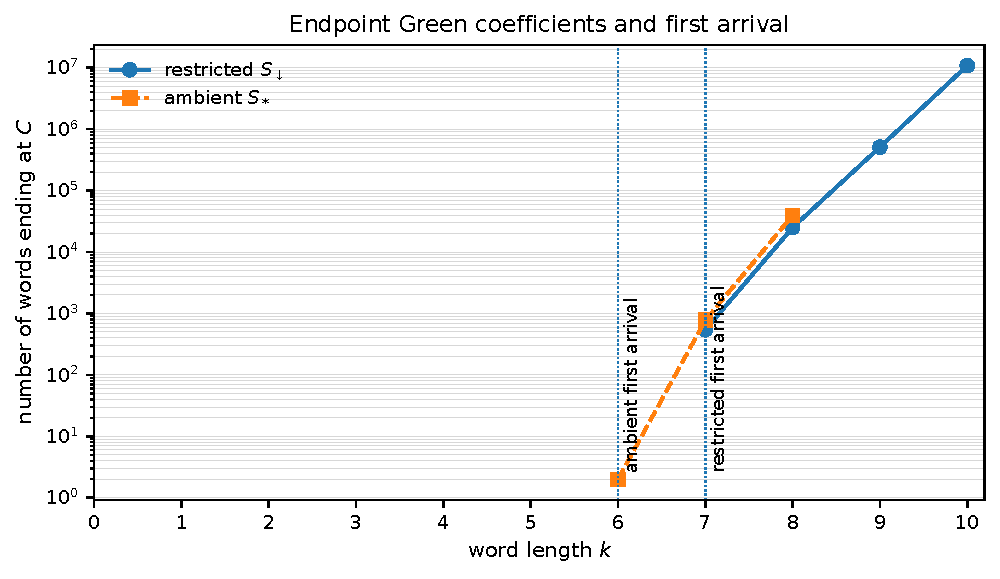
\includegraphics[width=.78\linewidth]{green_coefficients.pdf}
\caption{Exact endpoint word counts for the canonical target.  The ambient walk first arrives at length six.  The restricted walk first arrives at length seven.}
\label{fig:green-coefficients}
\end{figure}

Across the twenty defects, the truncated endpoint data split into five Green-signature classes, each of multiplicity four.  The signatures are listed in \cref{tab:green-signatures}.

\begin{table}[t]
\centering
\caption{The five endpoint Green-signature packets.  Each row occurs for four defective targets.}
\label{tab:green-signatures}
\resizebox{\textwidth}{!}{%
\begin{tabular}{@{}rrrrrrrr@{}}
\toprule
&\multicolumn{4}{c}{restricted coefficients}&\multicolumn{3}{c}{ambient coefficients}\\
packet&$[z^7]$&$[z^8]$&$[z^9]$&$[z^{10}]$&$[z^6]$&$[z^7]$&$[z^8]$\\
\midrule
1&326&15430&316118&7576819&4&570&23318\\
2&326&15536&321870&7727183&4&570&23318\\
3&543&25080&510703&10824940&2&776&39454\\
4&543&25639&511524&10984988&2&776&39454\\
5&543&26091&511819&11121486&2&776&39454\\
\bottomrule
\end{tabular}}
\end{table}

\section{Interval-tree certificates and connected higher-dimensional families}\label{sec:higher}

From this point through the rank and tensor arguments, the coefficient domain is a field $\F$.  The six-row atom is the first defect, but it is not an isolated low-dimensional accident.  This section gives a field-independent family of connected targets in every dimension at least seven.  The lower bound is certified by a multiscale rank potential adapted to the ordered flag.

\subsection{Interval-tree rank potential}

\begin{definition}[Interval tree]
An \emph{interval tree} on the ordered coordinates $0,1,\ldots,n-1$ is a rooted binary tree whose leaves occur in that order and whose every node is a contiguous interval.  If an internal node $v$ splits its interval into consecutive left and right children $L_v$ and $R_v$, define
\begin{equation}\label{eq:tree-potential}
\Phi_T(A)
=
\sum_{v\in\operatorname{Int}(T)}
\rank A[R_v,L_v],
\qquad A\in\U_n(\F).
\end{equation}
\end{definition}

\begin{lemma}[One-cut locality]\label{lem:one-cut-locality}
Let $X\in\U_n(\F)$ and let $X'$ be obtained from $X$ by one lower-directed transvection.  Then
\[
\bigl|\Phi_T(X')-\Phi_T(X)\bigr|\le1.
\]
\end{lemma}

\begin{proof}
Suppose the gate is $s\to t$ with $s<t$.  Let $v_0$ be the lowest node of $T$ whose two children separate $s$ and $t$.  The order of the leaves forces $s\in L_{v_0}$ and $t\in R_{v_0}$.  At this one node, a single row of the cross block $X[R_{v_0},L_{v_0}]$ changes, so its rank changes by at most one.

At every ancestor of $v_0$, the two rows lie in the same child.  If that child is the right child, the gate is an internal row operation on the relevant cross block and preserves rank; if it is the left child, the cross block is unchanged.  At a descendant containing $t$ but not $s$, every column of the descendant interval lies strictly to the right of $s$.  Since $X$ remains lower triangular, row $s$ vanishes on those columns, so the descendant block is unchanged.  All other descendants are also unchanged.  Hence only the term at $v_0$ can vary.
\end{proof}

\begin{corollary}[Interval-tree lower bound]\label{cor:tree-lower-bound}
For every $A\in\U_n(\F)$ and every interval tree $T$,
\[
\ellDown(A)\ge\Phi_T(A).
\]
\end{corollary}

\begin{proof}
The identity has potential zero.  Apply \cref{lem:one-cut-locality} along any lower-directed word from the identity to $A$.
\end{proof}

\begin{definition}[Tree-tight target]\label{def:tree-tight}
A lower-unitriangular target $A$ is \emph{tree tight} if some interval tree $T$ satisfies
\[
\Phi_T(A)=\ellDown(A).
\]
\end{definition}

Tree tightness is stronger than possessing a rank lower bound.  It says that one ordered hierarchy accounts for the entire restricted word length.  The family below is tree tight by construction.

\subsection{The snapshot family}

Fix integers
\[
u\ge1,
\qquad
1\le v\le u+1,
\]
and choose distinct phases
\[
0\le s_1<s_2<\cdots<s_v\le u.
\]
Order the coordinates as
\[
x_1,\ldots,x_u,\ p,\ q,\ t_1,\ldots,t_v.
\]
For $0\le s\le u$, put
\begin{equation}\label{eq:prefix-state}
w_s=e_p+\sum_{i=1}^{s}e_{x_i}.
\end{equation}
Define
\begin{equation}\label{eq:snapshot-target}
A(u;s_1,\ldots,s_v)\in\U_{u+v+2}(\F)
\end{equation}
by
\[
R_{x_i}=e_{x_i},
\qquad
R_p=w_u,
\qquad
R_q=e_q,
\]
and
\begin{equation}\label{eq:snapshot-output}
R_{t_j}=e_{t_j}+e_q+w_{s_j}
\qquad(1\le j\le v).
\end{equation}
The output rows record selected intermediate versions of the carrier $p$.

\begin{proof}[Proof of \cref{thm:snapshot-family}]
For the ambient construction, first apply
\[
q\to p.
\]
Sweep through the updates
\[
x_1\to p,\ldots,x_u\to p.
\]
Whenever phase $s_j$ is reached, apply
\[
p\to t_j.
\]
Finally apply $q\to p$ with coefficient $-1$.  At phase $s$, the carrier is $e_q+w_s$, so every output has the required value, and the final gate removes $e_q$ from row $p$.  The word has length
\[
1+u+v+1=u+v+2.
\]
Thus
\[
\ellAll\bigl(A(u;s_1,\ldots,s_v)\bigr)\le u+v+2.
\]

For a lower word, perform the same $u$ updates without opening the catalyst.  At each selected phase, use the two gates
\[
p\to t_j,
\qquad
q\to t_j.
\]
This gives length $u+2v$.

It remains to prove optimality in the lower model.  At the root, split
\[
\{x_1,\ldots,x_u,p\}
\quad\big|\quad
\{q,t_1,\ldots,t_v\}.
\]
The nonzero rows of the root cross block are $w_{s_1},\ldots,w_{s_v}$.  Distinct prefix vectors are linearly independent: in a linear relation, inspect successively a coordinate occurring in $w_{s_j}$ but in none of the earlier prefixes, starting from the largest phase.  Hence the root contributes $v$.

Inside the left child, use the comb that splits off $x_1$, then $x_2$, and so on while retaining $p$ in the remaining interval.  Every one of the $u$ cuts has rank one because the final row $p$ contains every $x_i$.  Inside the right child, repeatedly split off the last output while retaining $q$ in the left interval.  Each of the $v$ cuts has rank one because every output contains $q$.  Therefore
\[
\Phi_T\bigl(A(u;s_1,\ldots,s_v)\bigr)
=v+u+v=u+2v.
\]
The interval-tree lower bound matches the displayed lower circuit.
\end{proof}

\begin{figure}[t]
\centering
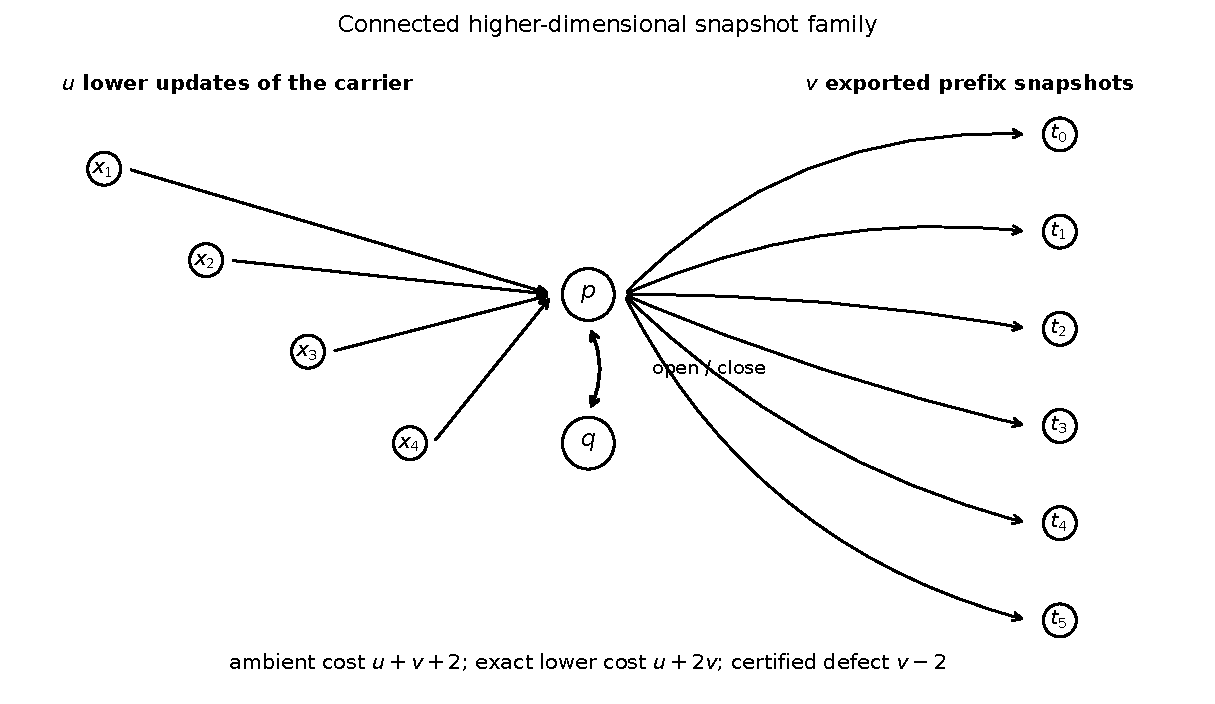
\includegraphics[width=.90\linewidth]{snapshot_family.pdf}
\caption{The connected snapshot family.  One temporary upper dependency lets the ambient circuit export $v$ selected prefix states.  A lower-only circuit must insert the $q$ component separately into every output.}
\label{fig:snapshot-family}
\end{figure}

\begin{remark}[Support connectivity]
For $u,v\ge1$, the undirected support graph of $A(u;s_1,\ldots,s_v)-I$ is connected.  Row $p$ joins all update coordinates $x_i$, while every output joins both $p$ and $q$.  The separation below therefore does not arise from a direct sum of independent six-row gadgets.
\end{remark}

\subsection{Exact higher binary examples}

The interval tree gives the exact restricted distance in all dimensions.  For the first three higher targets, a separate bidirectional search also proves that the displayed ambient construction is optimal.

\begin{theorem}[Exact binary cases in dimensions seven through nine]\label{thm:higher-exact}
Over $\F_2$, let
\[
H_7=A(2;0,1,2),
\qquad
H_8=A(3;0,1,2),
\qquad
H_9=A(3;0,1,2,3).
\]
Then
\[
(\ellDown(H_7),\ellAll(H_7))=(8,7),
\]
\[
(\ellDown(H_8),\ellAll(H_8))=(9,8),
\]
and
\[
(\ellDown(H_9),\ellAll(H_9))=(11,9).
\]
\end{theorem}

\begin{proof}
The restricted values follow from \cref{thm:snapshot-family}.  The ambient words have lengths $7$, $8$, and $9$.  To exclude shorter words, the supplement computes exact ambient balls and checks that the two relevant balls do not intersect.  The certificate sizes are
\begin{center}
\begin{tabular}{@{}ccll@{}}
\toprule
$n$&tested split&left ball&right ball\\
\midrule
$7$&$3+3$&$23276$&$23276$\\
$8$&$3+4$&$52277$&$1174097$\\
$9$&$4+4$&$2994949$&$2994949$\\
\bottomrule
\end{tabular}
\end{center}
Every intersection is empty.  Since the generating sets are symmetric, an empty radius-$r$ versus radius-$s$ intersection rules out every word of length at most $r+s$.
\end{proof}

These are exact higher-dimensional examples, not merely padded copies of $C$.

\subsection{A connected defect in every dimension}

\begin{proof}[Proof of \cref{cor:connected-gap}]
For $n\ge7$, put
\[
v_n=\left\lfloor\frac{n-1}{2}\right\rfloor,
\qquad
u_n=n-v_n-2,
\]
and take the phases
\[
0,1,\ldots,v_n-1.
\]
The inequality $v_n\le u_n+1$ holds, so the snapshot target is defined.  By \cref{thm:snapshot-family},
\[
\ellDown(A_n)=u_n+2v_n=n+v_n-2,
\]
while
\[
\ellAll(A_n)\le u_n+v_n+2=n.
\]
Hence
\[
\ellDown(A_n)-\ellAll(A_n)
\ge v_n-2
=
\left\lfloor\frac{n-5}{2}\right\rfloor.
\]
Connectivity follows from the preceding remark.
\end{proof}

\begin{table}[t]
\centering
\caption{Successive connected cases from the optimized snapshot family.  The restricted value is exact; the ambient column is a certified construction and is exact for $n=7,8,9$ over $\F_2$.}
\label{tab:higher-cases}
\begin{tabular}{@{}rrrrr@{}}
\toprule
$n$&$u$&$v$&$\ellDown$&ambient upper bound / certified gap\\
\midrule
$7$&$2$&$3$&$8$&$7\;/\;1$\\
$8$&$3$&$3$&$9$&$8\;/\;1$\\
$9$&$3$&$4$&$11$&$9\;/\;2$\\
$10$&$4$&$4$&$12$&$10\;/\;2$\\
$11$&$4$&$5$&$14$&$11\;/\;3$\\
$12$&$5$&$5$&$15$&$12\;/\;3$\\
$13$&$5$&$6$&$17$&$13\;/\;4$\\
$15$&$6$&$7$&$20$&$15\;/\;5$\\
$17$&$7$&$8$&$23$&$17\;/\;6$\\
$19$&$8$&$9$&$26$&$19\;/\;7$\\
$21$&$9$&$10$&$29$&$21\;/\;8$\\
\bottomrule
\end{tabular}
\end{table}

\begin{figure}[t]
\centering
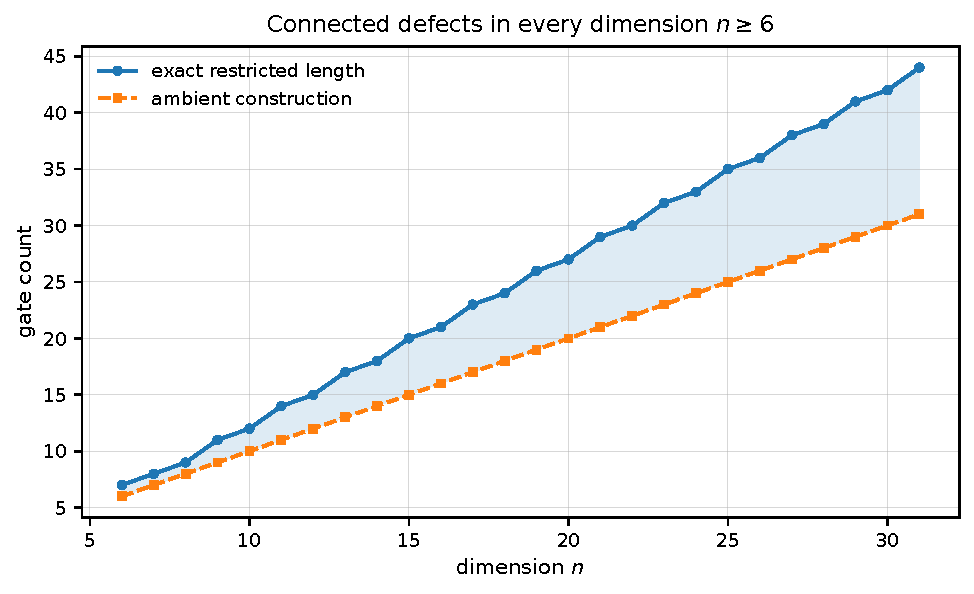
\includegraphics[width=.76\linewidth]{connected_higher_cases.pdf}
\caption{The six-row atom is the first exact defect.  From dimension seven onward, the connected snapshot family gives an exact restricted length and a shorter ambient construction in every dimension.}
\label{fig:higher-cases}
\end{figure}

The ratio also increases beyond the block-sum value $7/6$.

\begin{corollary}[Asymptotic multiplicative distortion]\label{cor:three-halves}
For every field,
\[
\limsup_{n\to\infty}
\sup_{A\in\U_n(\F),\,A\ne I}
\frac{\ellDown(A)}{\ellAll(A)}
\ge\frac32.
\]
\end{corollary}

\begin{proof}
Along the optimized connected family,
\[
\frac{\ellDown(A_n)}{\ellAll(A_n)}
\ge
\frac{n+\lfloor(n-1)/2\rfloor-2}{n},
\]
which tends to $3/2$.
\end{proof}

\section{Bounded and weighted catalytic resources}\label{sec:resources}

The connected snapshot family uses a single matched excursion: one upper-directed gate opens the dirty carrier and one upper-directed gate closes it.  This permits a sharper statement than the unrestricted inequality $\ellAll<\ellDown$.

\subsection{A bounded number of upper-directed gates}

For a circuit word $w$, let $u(w)$ denote its number of upper-directed gates.

\begin{definition}[Upper-gate budget]
For $q\ge0$ and $A\in\U_n(\F)$, define
\[
\ellBudget{q}(A)
=
\min\{|w|:[w]=A,\ u(w)\le q\}.
\]
Thus
\[
\ellBudget{0}(A)=\ellDown(A),
\qquad
\ellBudget{q+1}(A)\le\ellBudget{q}(A),
\qquad
\ellAll(A)\le\ellBudget{q}(A).
\]
\end{definition}

\begin{proposition}[Two upper gates give a linear advantage]\label{prop:two-upper-linear}
For every snapshot target $A=A(u;s_1,\ldots,s_v)$,
\[
\ellBudget{0}(A)=u+2v,
\qquad
\ellBudget{2}(A)\le u+v+2.
\]
Consequently,
\[
\ellBudget{0}(A)-\ellBudget{2}(A)\ge v-2.
\]
For the optimized connected target $A_n$ of \cref{cor:connected-gap},
\[
\ellBudget{0}(A_n)-\ellBudget{2}(A_n)
\ge
\left\lfloor\frac{n-5}{2}\right\rfloor.
\]
\end{proposition}

\begin{proof}
The exact restricted value is \cref{thm:snapshot-family}.  Its ambient construction has precisely two upper-directed gates, namely the opening and closing operations on the carrier row; all $u$ updates and all $v$ reads are lower directed.  The optimized choice has $v=\lfloor(n-1)/2\rfloor$.
\end{proof}

\begin{corollary}[No budget-only additive simulation bound]\label{cor:no-budget-only}
There is no finite constant $K$ such that
\[
\ellDown(A)\le\ellBudget{2}(A)+K
\]
for all dimensions, fields, and lower-unitriangular targets $A$.
\end{corollary}

\begin{proof}
The left-minus-right difference in \cref{prop:two-upper-linear} tends to infinity with $n$.
\end{proof}

Thus the power of the excursion is not controlled by the number of forbidden gates.  It is controlled by how many useful carrier states are exported between opening and closing.

\subsection{Rank-one, bandwidth-one flag escape}\label{subsec:microscopic-escape}

The number of upper gates does not measure how far a circuit travels from the lower subgroup.  We now control every intermediate state.

For $X\in\SL_n(\F)$, let $X^+$ be the matrix obtained by retaining only the strict upper entries of $X$.  Define
\[
r^+(X)=\rank X^+
\]
and
\[
b^+(X)=\max\{j-i:X_{ij}\ne0,\ i<j\},
\]
with $b^+(X)=0$ when $X^+=0$.  Let $\ellExc{r}{b}(A)$ be the minimum length of a transvection circuit from $I$ to $A$ such that every prefix matrix $X$ satisfies
\[
r^+(X)\le r,
\qquad
b^+(X)\le b.
\]

\begin{lemma}\label{lem:zero-excursion-equals-lower}
For $A\in\U_n(\F)$,
\[
\ellExc{0}{0}(A)=\ellDown(A).
\]
\end{lemma}

\begin{proof}
A lower-directed gate preserves lower triangularity.  Conversely, if $X$ is lower unitriangular and an upper-directed gate $R_t\leftarrow R_t+aR_s$ with $t<s$ is applied, then the new $(t,s)$ entry equals
\[
X_{t,s}+aX_{s,s}=a\ne0.
\]
The next state is therefore not lower triangular.  A circuit whose every prefix has zero strict upper part uses only lower-directed gates.
\end{proof}

\begin{theorem}[Microscopic escape, macroscopic saving]\label{thm:microscopic-escape}
For every field $\F$ and every $n\ge7$, there is a connected target $A_n\in\U_n(\F)$ such that
\[
\ellExc{0}{0}(A_n)-\ellExc{1}{1}(A_n)
\ge
\left\lfloor\frac{n-5}{2}\right\rfloor.
\]
The length-$n$ circuit witnessing the second term uses exactly two upper-directed gates.
\end{theorem}

\begin{proof}
Use the connected family from \cref{cor:connected-gap}, with the carrier coordinates $p<q$ adjacent.  Between the opening and closing gates, the only strict upper entry is the coefficient at position $(p,q)$.  Hence every prefix has upper rank at most one and upper bandwidth at most one.  The displayed ambient circuit has length $n$, whereas
\[
\ellExc{0}{0}(A_n)=\ellDown(A_n)
=n+\left\lfloor\frac{n-1}{2}\right\rfloor-2.
\]
Subtracting proves the claim.
\end{proof}

\begin{figure}[t]
\centering
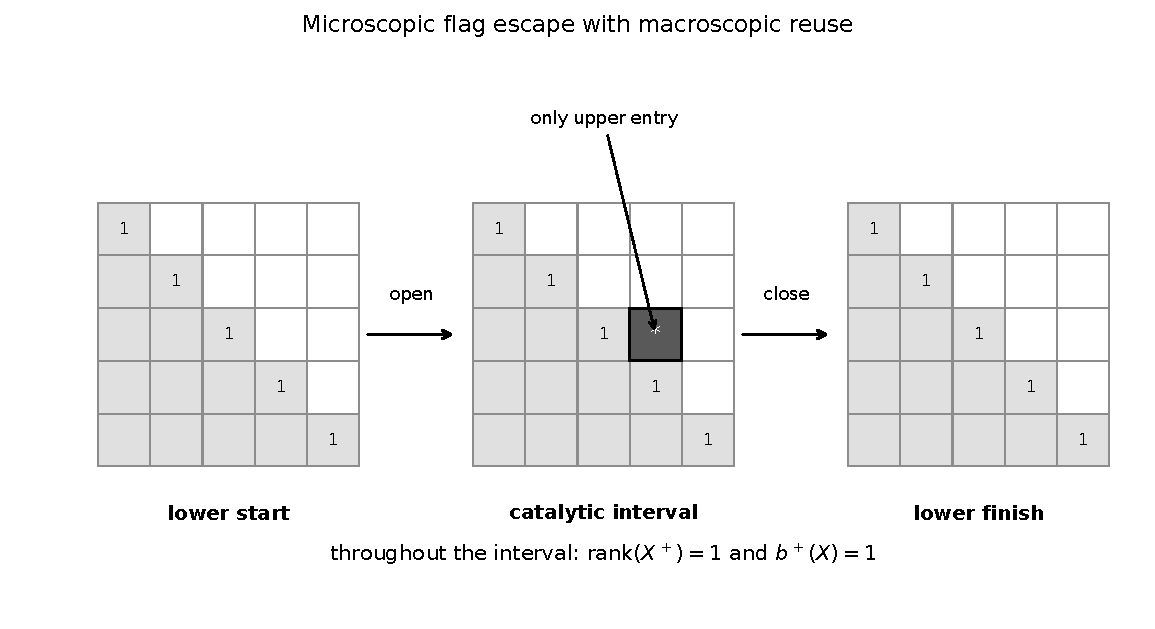
\includegraphics[width=.82\linewidth]{microscopic_escape.pdf}
\caption{The snapshot circuit leaves the lower subgroup through one adjacent upper entry.  Throughout the excursion the strict upper part has rank one and bandwidth one, yet the accumulated saving grows linearly.}
\label{fig:microscopic-escape}
\end{figure}

\subsection{A weighted upper-gate metric}

A hardware or fault model may penalize an upper-directed interaction more heavily than a lower-directed one.  Fix $\lambda>0$.  If $w$ has $d(w)$ lower-directed gates and $u(w)$ upper-directed gates, put
\[
\operatorname{cost}_{\lambda}(w)=d(w)+\lambda u(w),
\]
and define
\[
\ellWeight{\lambda}(A)
=
\inf\{\operatorname{cost}_{\lambda}(w):[w]=A\}.
\]
At $\lambda=1$ this is the ordinary ambient length, while large $\lambda$ increasingly penalizes flag excursions.

\begin{proposition}[Fixed penalties do not suppress catalysis]\label{prop:weighted-catalysis}
For every snapshot target $A=A(u;s_1,\ldots,s_v)$ and every $\lambda>0$,
\[
\ellWeight{\lambda}(A)
\le
u+v+2\lambda.
\]
Consequently,
\[
\ellDown(A)-\ellWeight{\lambda}(A)
\ge
v-2\lambda.
\]
For the optimized connected family,
\[
\ellDown(A_n)-\ellWeight{\lambda}(A_n)
\ge
\left\lfloor\frac{n-1}{2}\right\rfloor-2\lambda.
\]
In particular, for every fixed finite $\lambda$, the weighted advantage grows linearly with $n$.
\end{proposition}

\begin{proof}
The displayed catalytic word contains $u+v$ lower-directed gates and two upper-directed gates, so its weighted cost is $u+v+2\lambda$.  Subtract this from the exact restricted value $u+2v$.  The optimized family again has $v=\lfloor(n-1)/2\rfloor$.
\end{proof}

\begin{remark}[Penalty threshold]
For the displayed realization of a snapshot target, catalysis beats the optimal lower-only cost whenever
\[
\lambda<\frac v2.
\]
The critical penalty therefore scales with the number of consumers, not with the dimension of the dirty workspace.
\end{remark}

\begin{figure}[t]
\centering
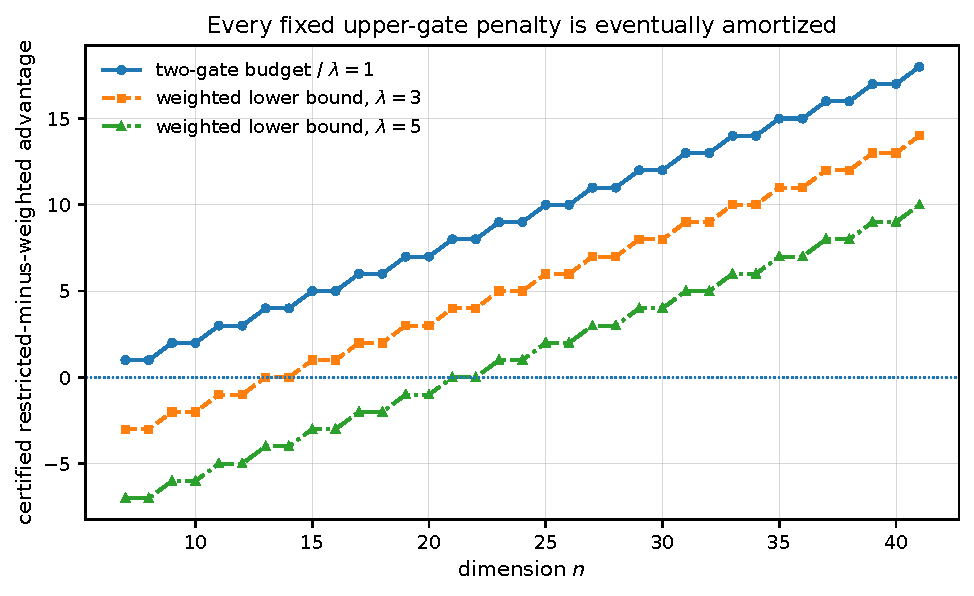
\includegraphics[width=.78\linewidth]{weighted_catalysis.pdf}
\caption{Certified lower-minus-weighted advantage for the optimized connected family.  Every fixed upper-gate penalty is eventually amortized because the same matched excursion serves a growing number of output snapshots.}
\label{fig:weighted-catalysis}
\end{figure}

\begin{proof}[Proof of \cref{thm:resource-robustness}]
Combine \cref{prop:two-upper-linear,prop:weighted-catalysis}.
\end{proof}


\section{Algebraic rarity of catalytic defects}\label{sec:rarity}

The preceding sections construct highly structured targets with large defects.  This section proves the complementary statement that catalytic defects are nongeneric at every fixed dimension.  Fix a field $K$.  Algebraic dimensions and closures are taken after base change to an algebraic closure of $K$.  Put
\[
N=\dim \U_n=\binom n2,
\qquad
M=n(n-1).
\]

\subsection{Transvection product loci}

For a direction skeleton
\[
\sigma=((t_1,s_1),\ldots,(t_L,s_L)),
\qquad t_i\ne s_i,
\]
define the polynomial word map
\[
\Phi_\sigma:\Aff^L\longrightarrow\SL_n,
\qquad
(a_1,\ldots,a_L)
\longmapsto
(I+a_LE_{t_L,s_L})\cdots(I+a_1E_{t_1,s_1}).
\]
The coefficients are allowed to vanish, so a word of length at most $L$ can be padded to length $L$.  Let
\[
\mathcal R^*_{n,\le L}
=
\U_n\cap
\bigcup_{\sigma\in\{(t,s):t\ne s\}^L}
\operatorname{im}\Phi_\sigma
\]
be the ambient reachability locus, and define $\mathcal R^\downarrow_{n,\le L}$ analogously using only lower directions.

Equivalently, put
\[
X_*
=
\bigcup_{t\ne s}\{I+aE_{t,s}:a\in K\},
\qquad
X_\downarrow
=
\bigcup_{s<t}\{I+aE_{t,s}:a\in K\}.
\]
Then $\ellAll(A)$ and $\ellDown(A)$ are the corresponding transvection product lengths: the least $L$ for which $A\in X_*^L$ or $A\in X_\downarrow^L$.

\begin{proposition}[Dimension of bounded-length loci]\label{prop:reachability-dimension}
For every $L\ge0$, the sets $\mathcal R^*_{n,\le L}$ and $\mathcal R^\downarrow_{n,\le L}$ are constructible and
\[
\dim\overline{\mathcal R^*_{n,\le L}}
\le L,
\qquad
\dim\overline{\mathcal R^\downarrow_{n,\le L}}
\le L.
\]
\end{proposition}

\begin{proof}
There are finitely many direction skeletons of length $L$.  For each skeleton, $\Phi_\sigma$ is a morphism from an $L$-dimensional affine space.  Chevalley's theorem makes its image constructible, and the closure of the image has dimension at most $L$ \cite{Hartshorne1977}.  Finite unions preserve constructibility and the maximum dimension bound.  Intersecting with the closed subvariety $\U_n$ cannot increase dimension.
\end{proof}

The argument is an instance of a general parameter-counting principle.

\begin{proposition}[Dimension per gate]\label{prop:dimension-per-gate}
Let $G$ be an algebraic group, let $V\subseteq G$ be an irreducible subvariety of dimension $D$, and let $X\subseteq G$ be a finite union of locally closed subvarieties, each of dimension at most $r$, with the identity in $X$.  Write
\[
X^{(L)}
=
\{x_L\cdots x_1:x_1,\ldots,x_L\in X\}.
\]
Then
\[
\dim\overline{V\cap X^{(L)}}\le rL.
\]
In particular, if $rL<D$, a Zariski-generic point of $V$ has $X$-product length greater than $L$.
\end{proposition}

\begin{proof}
Every irreducible component of the Cartesian power $X^{\times L}$ has dimension at most $rL$.  Multiplication $G^L\to G$ is a morphism, so the closure of the image of each component has dimension at most $rL$.  There are finitely many components, and intersecting the resulting finite union with $V$ cannot increase dimension.  Since the identity belongs to $X$, products of length at most $L$ are already contained in $X^{(L)}$.
\end{proof}

For transvections, the discrete choice of direction contributes finitely many components and each component carries one scalar parameter.  Thus $r=1$.  Every element of $\U_n(K)$ has lower length at most $N$: process the strict lower entries in any root order compatible with elimination.  The dimension-per-gate bound shows that this worst-case value is generic.

\begin{theorem}[Generic rigidity]\label{thm:generic-rigidity}
Let $K$ be an infinite field.  There is a nonempty Zariski-open subvariety $\Omega_n\subseteq\U_n$, defined over $K$, such that $\Omega_n(K)$ is nonempty and
\[
\ellAll(A)=\ellDown(A)=N
\qquad(A\in\Omega_n(K)).
\]
The same statement holds with exact product length replaced by border product length.
\end{theorem}

\begin{proof}
After base change to an algebraic closure $\overline K$, \cref{prop:reachability-dimension} gives
\[
\dim\overline{\mathcal R^*_{n,\le N-1}}\le N-1<N=\dim\U_n.
\]
Because the word maps are defined over $K$, this proper closed set descends to a proper closed subset of $\U_n$ over $K$.  Its complement is a nonempty Zariski-open set $\Omega_n$.  Since $K$ is infinite and $\U_n\cong\Aff^N$, the set $\Omega_n(K)$ is nonempty and Zariski dense.  For any $A\in\Omega_n(K)$, one has $\ellAll(A)\ge N$.  The inequalities
\[
\ellAll(A)\le\ellDown(A)\le N
\]
force equality.  Replacing each image by its Zariski closure gives the border-length statement by the same argument.
\end{proof}

\subsection{Defect codimension}

For an algebraically closed field $K$ and $d\ge1$, define
\[
\mathcal D_{n,\ge d}
=
\{A\in\U_n(K):\DeltaDef(A)\ge d\}.
\]

\begin{theorem}[Defect--codimension bound]\label{thm:defect-codimension}
Let $K$ be algebraically closed.  For every $1\le d\le N$,
\[
\dim\overline{\mathcal D_{n,\ge d}}\le N-d.
\]
Equivalently,
\[
\codim_{\U_n}\overline{\mathcal D_{n,\ge d}}\ge d.
\]
More finely, on the stratum where $\ellDown(A)=L$ and $\DeltaDef(A)\ge d$, the closure has dimension at most $L-d$.
\end{theorem}

\begin{proof}
If $\DeltaDef(A)\ge d$, then
\[
\ellAll(A)
\le
\ellDown(A)-d
\le
N-d.
\]
Thus $\mathcal D_{n,\ge d}\subseteq\mathcal R^*_{n,\le N-d}$, and \cref{prop:reachability-dimension} gives the first assertion.  On the intrinsic-length-$L$ stratum one instead has $\ellAll(A)\le L-d$, proving the refinement.
\end{proof}

\begin{figure}[t]
\centering
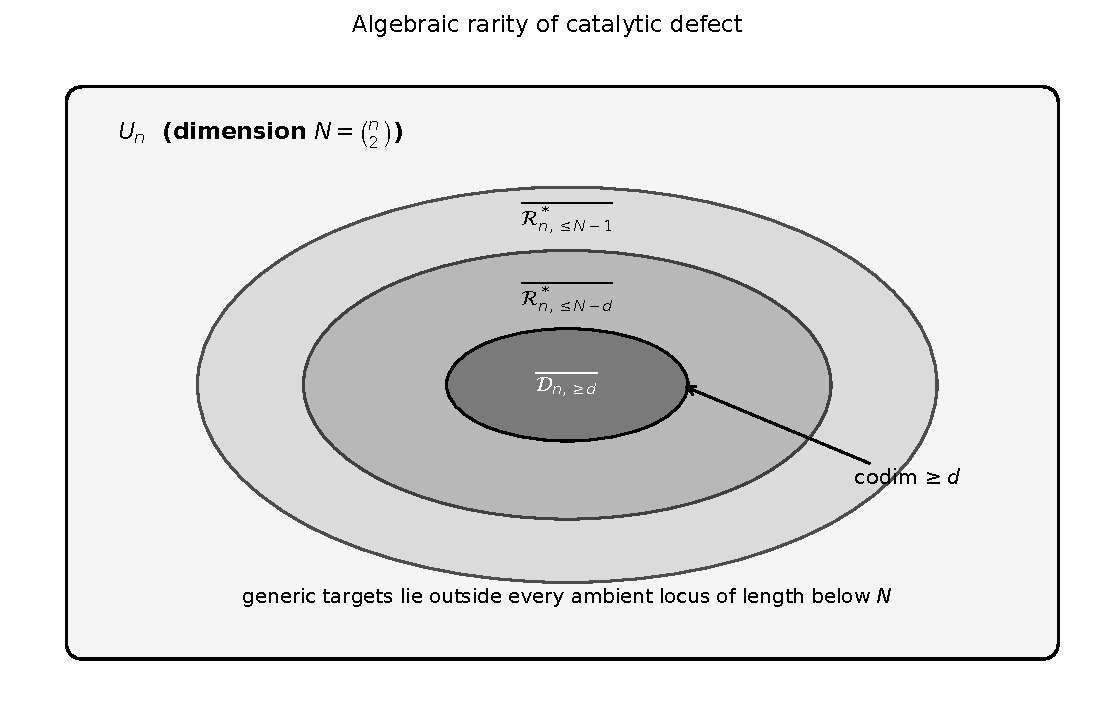
\includegraphics[width=.78\linewidth]{defect_strata.pdf}
\caption{Bounded ambient product loci form nested algebraic strata inside $\U_n$.  A defect of size at least $d$ lies inside the ambient reachability locus of length $N-d$, whose closure has codimension at least $d$.}
\label{fig:defect-strata}
\end{figure}

\subsection{Finite-field sparsity}

The dimension argument has an elementary counting counterpart.  Allowing zero coefficients, a padded word of length $L$ is specified by $L$ choices among $M$ directed positions and $L$ coefficients in $\F_q$.  Consequently
\[
|\mathcal R^*_{n,\le L}(\F_q)|\le(Mq)^L.
\]

\begin{corollary}[Finite-field defect density]\label{cor:finite-field-density}
For $1\le d\le N$,
\[
\Prob_{A\in\U_n(\F_q)}[\DeltaDef(A)\ge d]
\le
\min\{1,M^{N-d}q^{-d}\}.
\]
In particular, for fixed $n$,
\[
\Prob[\DeltaDef(A)>0]=O_n(q^{-1}),
\qquad
\Exp[\DeltaDef(A)]=O_n(q^{-1})
\]
as $q\to\infty$.
\end{corollary}

\begin{proof}
The defect condition implies ambient length at most $N-d$, so the number of such targets is at most $(Mq)^{N-d}$.  Divide by
\[
|\U_n(\F_q)|=q^N.
\]
The expectation bound follows from
\[
\Exp[\DeltaDef]=\sum_{d=1}^{N}\Prob[\DeltaDef\ge d].
\]
\end{proof}

The same counting argument also gives
\[
\Prob_{A\in\U_n(\F_q)}[\ellAll(A)=\ellDown(A)=N]
\ge
1-M^{N-1}q^{-1},
\]
whenever the right side is positive.  Thus maximal ambient and intrinsic length is not only Zariski generic over infinite fields but asymptotically typical over growing finite fields at fixed dimension.

\subsection{Border catalysis}

For an algebraic generating set $X$, define the border product length
\[
\underline\ell_X(A)
=
\min\{L:A\in\overline{X^L}\}.
\]
This is analogous to the passage from tensor rank to border rank \cite{Landsberg2012}.  The generic value is still $N$ by \cref{thm:generic-rigidity}, but exact and border defects can differ on exceptional strata.  It is presently open whether the canonical atom $C$ belongs to the closure of the six-factor lower transvection locus.  A negative answer would show that its one-gate defect is stable under algebraic degeneration; a positive answer would exhibit a rank-versus-border-rank phenomenon inside reversible linear synthesis.

\begin{remark}[Rare but amplifiable]\label{rem:rare-amplifiable}
The codimension theorem and the tensor construction point in opposite directions without contradiction.  At each fixed $n$, a defect of size $d$ lies on a codimension-at-least-$d$ subset.  Carefully selected points on these thin strata can nevertheless be tensorized into families with $\Omega(n\log n)$ additive defect.  Catalytic compression is therefore algebraically rare but asymptotically amplifiable.
\end{remark}

\section{Recursive, block, and tensor amplification}\label{sec:amplification}

\subsection{Restricted block additivity}

The lower metric is exactly additive on contiguous block-diagonal targets.

\begin{proposition}[Block additivity]\label{prop:block-additivity}
Let $A_i\in\U_{n_i}(\F)$ for $1\le i\le k$.  Then
\[
\ellDown\bigl(\operatorname{diag}(A_1,\ldots,A_k)\bigr)
=
\sum_{i=1}^k\ellDown(A_i).
\]
\end{proposition}

\begin{proof}
The upper bound follows by running optimal lower circuits independently inside the blocks.

For the lower bound, view an element of $\U_{n_1+\cdots+n_k}(\F)$ as a lower block-triangular matrix and project to its diagonal blocks:
\[
\pi(X)=(X_{11},\ldots,X_{kk}).
\]
Because diagonal blocks multiply independently in a lower block-triangular product, $\pi$ is a homomorphism.  A lower transvection internal to one block projects to one generator in that factor, while a crossing transvection projects to the identity in every factor.  If $m_i$ gates survive in factor $i$, then the total word length is at least
\[
\sum_i m_i
\ge
\sum_i\ellDown(A_i).
\]
\end{proof}

The ambient metric is subadditive:
\[
\ellAll\bigl(\operatorname{diag}(A_1,\ldots,A_k)\bigr)
\le
\sum_i\ellAll(A_i).
\]
Cross-block ambient workspace can only improve this upper bound.

\begin{corollary}[Block-sum amplification]\label{cor:linear-gap}
For every field and every $n\ge6$, there is an $A_n\in\U_n(\F)$ with
\[
\ellDown(A_n)-\ellAll(A_n)
\ge
\left\lfloor\frac n6\right\rfloor.
\]
For $n=6k$, the target $C^{\oplus k}$ satisfies
\[
\ellDown(C^{\oplus k})=7k,
\qquad
\ellAll(C^{\oplus k})\le6k.
\]
\end{corollary}

\begin{proof}
For $n=6k+r$, take $C^{\oplus k}\oplus I_r$ and apply block additivity together with $k$ copies of the ambient six-gate word.
\end{proof}

\begin{figure}[t]
\centering
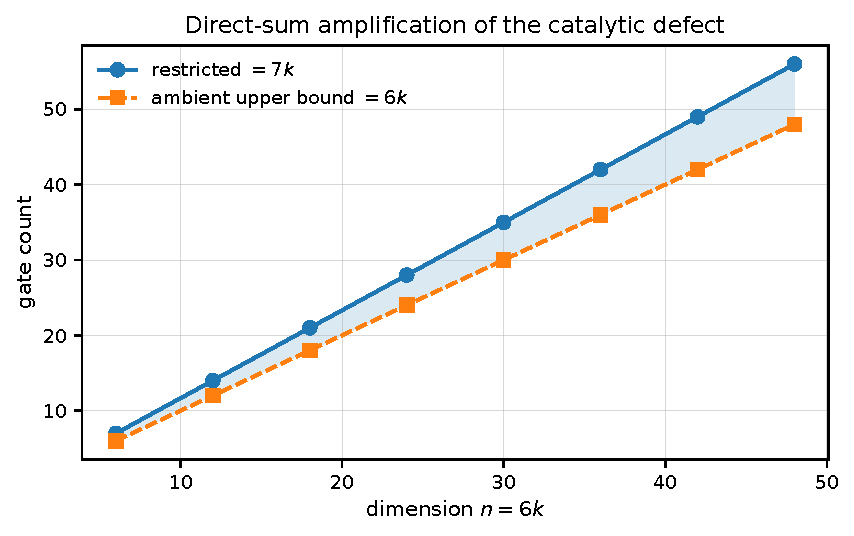
\includegraphics[width=.68\linewidth]{direct_sum_amplification.pdf}
\caption{Block-sum amplification.  The restricted length is exactly $7k$, while the displayed ambient construction has length $6k$.}
\label{fig:direct-sum}
\end{figure}

\subsection{A recursive zeta-shaped lift}

For $A\in\U_m(\F)$, define
\begin{equation}\label{eq:zeta-lift}
\mathcal Z(A)
=
\begin{pmatrix}
A&0\\
A&A
\end{pmatrix}
\in\U_{2m}(\F).
\end{equation}

\begin{proposition}[Exact restricted lift]\label{prop:zeta-lift}
For every $A\in\U_m(\F)$,
\[
\ellDown(\mathcal Z(A))=2\ellDown(A)+m,
\]
and
\[
\ellAll(\mathcal Z(A))\le2\ellAll(A)+m.
\]
Consequently,
\[
\DeltaDef(\mathcal Z(A))\ge2\DeltaDef(A).
\]
\end{proposition}

\begin{proof}
The construction first realizes $\operatorname{diag}(A,A)$ and then applies the $m$ root-cross gates that add top row $i$ into bottom row $i$.

For the lower bound, write a circuit state in $m\times m$ blocks as
\[
X=
\begin{pmatrix}
P&0\\
Q&R
\end{pmatrix}.
\]
Projection to the two diagonal blocks forces at least $2\ellDown(A)$ internal gates.  A top-internal gate leaves $Q$ unchanged.  A bottom-internal gate performs an invertible row operation on $Q$ and preserves its rank.  A root-cross gate changes $Q$ by one rank-one row contribution, so it can increase $\rank Q$ by at most one.  The final cross block is $A$, of rank $m$, hence at least $m$ root-cross gates are necessary.
\end{proof}

Let $A^{[0]}=A$ and $A^{[r+1]}=\mathcal Z(A^{[r]})$.  If $A$ has size $m$, restricted length $a$, and ambient length $b$, then
\begin{equation}\label{eq:zeta-iterate}
\ellDown(A^{[r]})
=
2^r a+r m2^{r-1},
\end{equation}
and
\begin{equation}\label{eq:zeta-iterate-ambient}
\ellAll(A^{[r]})
\le
2^r b+r m2^{r-1}.
\end{equation}
Thus
\[
\DeltaDef(A^{[r]})\ge2^r\DeltaDef(A).
\]
For the canonical atom $C$, the first values are
\begin{center}
\begin{tabular}{@{}rrrrr@{}}
\toprule
$r$&dimension&restricted exact&ambient upper bound&certified gap\\
\midrule
$0$&$6$&$7$&$6$&$1$\\
$1$&$12$&$20$&$18$&$2$\\
$2$&$24$&$52$&$48$&$4$\\
$3$&$48$&$128$&$120$&$8$\\
$4$&$96$&$304$&$288$&$16$\\
\bottomrule
\end{tabular}
\end{center}
This gives arbitrarily deep exact recursion with identical diagonal children and a full-rank cross block while preserving a positive defect.

\begin{figure}[t]
\centering
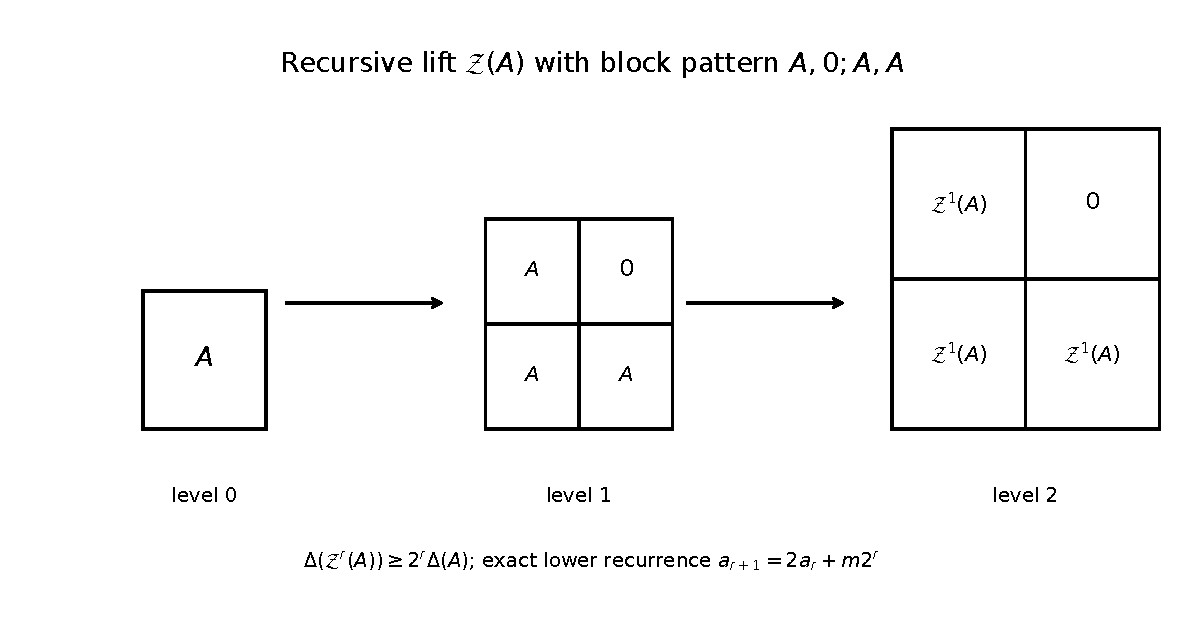
\includegraphics[width=.88\linewidth]{recursive_zeta_lift.pdf}
\caption{The recursive lift has the same outer shape as a Boolean zeta recursion.  A finite defect at the leaf is doubled at every lift.}
\label{fig:zeta-lift}
\end{figure}

\subsection{Tensor products of tree-tight targets}

The tensor operation gives the stronger asymptotic amplification.

\begin{theorem}[Exact restricted tensor rule]\label{thm:tensor-rule}
Let $A\in\U_m(\F)$ and $B\in\U_n(\F)$ be tree tight.  Then $A\otimes B$ is tree tight and
\begin{equation}\label{eq:tensor-lower}
\ellDown(A\otimes B)
=
n\ellDown(A)+m\ellDown(B).
\end{equation}
Moreover,
\begin{equation}\label{eq:tensor-ambient}
\ellAll(A\otimes B)
\le
n\ellAll(A)+m\ellAll(B),
\end{equation}
so
\begin{equation}\label{eq:tensor-defect}
\DeltaDef(A\otimes B)
\ge
n\DeltaDef(A)+m\DeltaDef(B).
\end{equation}
\end{theorem}

\begin{proof}
Use lexicographic order on the $mn$ coordinates.  Substitute a copy of a certificate tree for $B$ at every leaf of a certificate tree for $A$.  At an outer node, the cross block is
\[
A[R,L]\otimes B,
\]
whose rank is $n\rank A[R,L]$ because $B$ is invertible.  The outer nodes therefore contribute $n\ellDown(A)$.  The $m$ diagonal copies of the inner tree contribute $m\ellDown(B)$.  This proves the lower bound.

For the matching lower construction, first realize $I_m\otimes B$ using $m$ copies of a circuit for $B$.  Then realize $A\otimes I_n$.  Each gate of a circuit for $A$ lifts to $n$ coordinatewise gates.  Since
\[
(A\otimes I_n)(I_m\otimes B)=A\otimes B,
\]
the cost is the right side of \cref{eq:tensor-lower}.  The same construction with ambient circuits proves \cref{eq:tensor-ambient}.
\end{proof}

If $A$ is tree tight of dimension $m$, with restricted length $a$ and an ambient construction of length $b$, then
\begin{equation}\label{eq:tensor-power-lower}
\ellDown(A^{\otimes r})
=
r m^{r-1}a,
\end{equation}
and
\begin{equation}\label{eq:tensor-power-upper}
\ellAll(A^{\otimes r})
\le
r m^{r-1}b.
\end{equation}
A positive one-copy defect therefore becomes an order-$N\log N$ defect at dimension $N=m^r$.

\begin{proof}[Proof of \cref{thm:tensor-main}]
Apply \cref{thm:tensor-rule} repeatedly to the tree-tight snapshot target $A=A(u;s_1,\ldots,s_v)$, for which
\[
a=u+2v,
\qquad
b=u+v+2=m.
\]
Then
\[
\ellDown(A^{\otimes r})
-
\ellAll(A^{\otimes r})
\ge
r m^{r-1}(v-2).
\]
Since $N=m^r$ and $r=\log_2N/\log_2m$, this is
\[
\frac{v-2}{m\log_2m}N\log_2N.
\]
\end{proof}

Within the snapshot family, the best coefficient is obtained by the twenty-one-dimensional seed
\[
A_{21}=A(9;0,1,\ldots,9),
\]
for which
\[
\ellDown(A_{21})=29,
\qquad
\ellAll(A_{21})\le21,
\qquad
\DeltaDef(A_{21})\ge8.
\]

\begin{proposition}[Optimal snapshot seed for tensor rate]\label{prop:optimal-snapshot-seed}
Among all snapshot targets, the coefficient
\[
\frac{v-2}{m\log_2m},
\qquad m=u+v+2,
\]
is maximized at
\[
(m,u,v)=(21,9,10).
\]
\end{proposition}

\begin{proof}
For fixed $m$, maximize $v$ subject to $v\le u+1$ and $u+v+2=m$.  Thus
\[
v=\left\lfloor\frac{m-1}{2}\right\rfloor.
\]
If $m$ is even and at least eight, its coefficient is strictly smaller than that of $m-1$, because the numerator is the same while
\[
(m-1)\log(m-1)<m\log m.
\]
It therefore suffices to consider odd $m$.  Apart from the constant change of logarithm base, the odd-dimensional envelope is
\[
f(x)=\frac{x-5}{2x\log x}.
\]
Its derivative has the sign of
\[
5(1+\log x)-x.
\]
For $x>5$ this expression crosses zero exactly once, between $19$ and $21$.  Direct comparison gives $f(21)>f(19)$, after which the envelope decreases.  Hence the unique integer maximizer is $m=21$.
\end{proof}

The first tensor powers are
\begin{center}
\begin{tabular}{@{}rrrrr@{}}
\toprule
$r$&dimension $21^r$&restricted exact&ambient upper bound&certified gap\\
\midrule
$1$&$21$&$29$&$21$&$8$\\
$2$&$441$&$1218$&$882$&$336$\\
$3$&$9261$&$38367$&$27783$&$10584$\\
$4$&$194481$&$1074276$&$777924$&$296352$\\
\bottomrule
\end{tabular}
\end{center}

\begin{figure}[t]
\centering
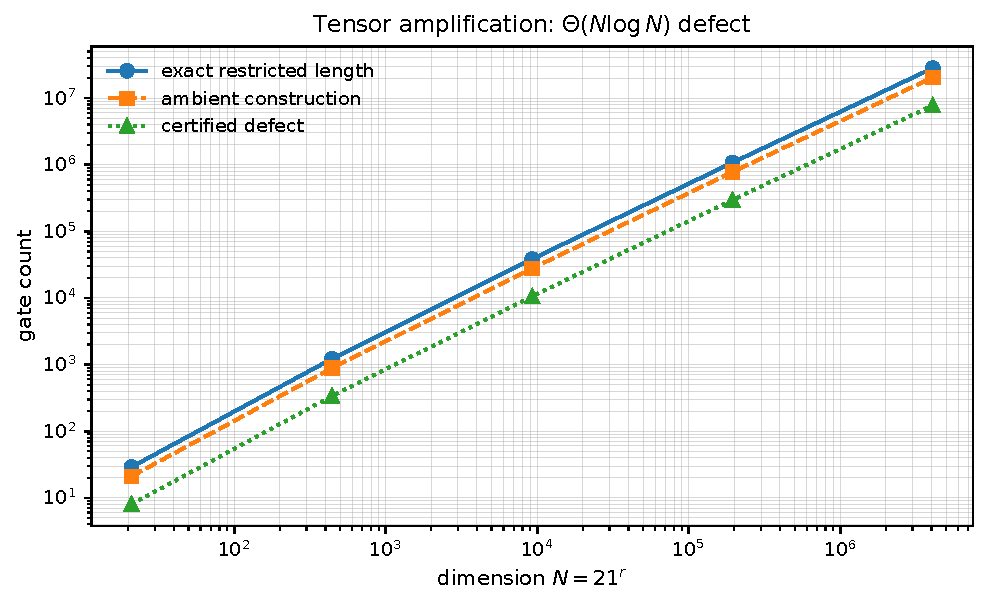
\includegraphics[width=.74\linewidth]{tensor_amplification.pdf}
\caption{Tensor powers of the twenty-one-dimensional snapshot seed.  Both displayed circuit sizes are of order $N\log N$, and their difference has a positive $N\log N$ coefficient.}
\label{fig:tensor-amplification}
\end{figure}

\subsection{Stable tensor capacity and activation}\label{subsec:stable-tensor}

The tensor inequality also defines a regularized ambient invariant.  Let $A\in\U_m(\F)$ and put
\[
b_r(A)
=
\frac{\ellAll(A^{\otimes r})}{m^{r-1}}.
\]
Applying \cref{eq:tensor-ambient} to $A^{\otimes r}\otimes A^{\otimes s}$ gives
\[
b_{r+s}(A)\le b_r(A)+b_s(A).
\]

\begin{proposition}[Stable tensor length]\label{prop:stable-tensor-length}
The limit
\[
\tau_*(A)
=
\lim_{r\to\infty}
\frac{\ellAll(A^{\otimes r})}{r m^{r-1}}
=
\inf_{r\ge1}
\frac{\ellAll(A^{\otimes r})}{r m^{r-1}}
\]
exists.  If $A$ is tree tight, then the stable catalytic capacity
\[
\kappa_\otimes(A)
=
\ellDown(A)-\tau_*(A)
\]
satisfies
\[
\kappa_\otimes(A)\ge\DeltaDef(A).
\]
\end{proposition}

\begin{proof}
The sequence $b_r(A)$ is subadditive, so Fekete's lemma gives the displayed limit.  Since the one-copy lifted construction implies $\tau_*(A)\le\ellAll(A)$, one has
\[
\kappa_\otimes(A)
\ge
\ellDown(A)-\ellAll(A)
=
\DeltaDef(A).
\]
For a tree-tight target, \cref{eq:tensor-power-lower} identifies $\ellDown(A)$ with its exact normalized restricted tensor cost.
\end{proof}

For the twenty-one-dimensional seed $A_{21}$,
\[
\kappa_\otimes(A_{21})\ge8.
\]
This regularization introduces a new possibility: a target may have $\DeltaDef(A)=0$ but $\kappa_\otimes(A)>0$.  In that case one copy is rigid while many tensor copies admit a collective shortcut.  We call this \emph{tensor activation}.

\subsection{Extremal consequences}

Define
\[
D_n(\F)
=
\sup_{A\in\U_n(\F)}
\bigl(\ellDown(A)-\ellAll(A)\bigr).
\]
For finite fields the supremum is a maximum.  The tensor family gives the following explicit all-dimension bound.

\begin{proof}[Proof of \cref{cor:nlogn-gap}]
Let $m=21$ and write
\[
n=\sum_{j=0}^{r}d_jm^j,
\qquad
0\le d_j<m.
\]
Take the block sum of $d_j$ copies of $A_{21}^{\otimes j}$ for every $j$, with the convention $A_{21}^{\otimes0}=I_1$.  Block additivity and the tensor estimate give
\[
D_n(\F)
\ge
\frac{8}{21}
\sum_{j=0}^{r}j d_j21^j.
\]
Put $S=\sum_j j d_j21^j$.  Since $r=\lfloor\log_{21}n\rfloor$,
\[
r n-S
=
\sum_{j<r}(r-j)d_j21^j
\le
20\sum_{h\ge1}h21^{r-h}
\le
\frac{21^{r+1}}{20}
\le
\frac{21}{20}n.
\]
Also $r\ge\log_{21}n-1$.  Therefore
\[
S\ge n\log_{21}n-\frac{41}{20}n.
\]
Multiplying by $8/21$ yields
\[
D_n(\F)
\ge
\frac{8}{21\log_2 21}n\log_2n
-
\frac{82}{105}n.
\]
\end{proof}

Numerically,
\[
\frac{8}{21\log_2 21}
=0.0867315\ldots.
\]
The elementary bottom-to-top construction gives
\[
D_n(\F)\le\frac{n(n-1)}2.
\]
Thus the current general range is
\begin{equation}\label{eq:defect-range}
0.0867315\,n\log_2n-O(n)
\le
D_n(\F)
\le
\frac{n(n-1)}2.
\end{equation}

\section{Discussion and open problems}\label{sec:discussion}

\subsection{What the threshold and higher families establish}

The six-row atom proves that an optimal circuit for a lower-unitriangular target need not remain in the lower-unitriangular subgroup.  The exact binary classification shows that this first failure is rigid: it occurs for exactly twenty targets, every defect is $(7,6)$, and every target is generated by the same three-cross, one-phase mechanism.

The higher-dimensional results change the scale of the phenomenon.  The connected snapshot family shows that exactly two upper-directed gates can support a defect linear in dimension, and that the advantage persists under every fixed finite penalty on those gates.  The recursive lift shows that a defective leaf survives arbitrarily many identical full-rank dyadic levels.  Tensor products then turn any tree-tight positive-defect atom into an order-$N\log N$ additive separation.  Thus the defect is not a finite anomaly and not merely linear in the worst case.  At the same time, generic rigidity and the defect--codimension theorem show that large defects require correspondingly special algebraic conditions.  The central synthesis is therefore not ubiquity but amplification: thin exceptional strata can control large structured families.

\subsection{Relation to ordinary CNOT synthesis}

Exact CNOT synthesis usually minimizes $\ellAll$ on all of $\GL_n(\F_2)$.  The present problem fixes a structured target class and compares the ambient optimum with a structure-preserving optimum.  Recent exact methods explore the full Cayley graph using symmetries, bidirectional search, A* methods, SAT, and related techniques \cite{ChristensenEtAl2025,WebsterEtAl2025,ShaikVanDePol2025}.  The right-coset computation in this paper is tailored to a subgroup comparison, while the higher-dimensional exact audits use direct bidirectional balls for selected targets.

The 2026 NP-completeness result for all-to-all CNOT distance shows that cancellation and unrestricted parity reuse must be handled in full generality \cite{AcuavivaEtAl2026}.  The present constructions isolate explicit reusable-carrier mechanisms under an ordered restriction.  They do not resolve ambient synthesis complexity.

\subsection{Open directions}

\begin{question}[Universal six-dimensional threshold]
Is six the first defective dimension over every field, or even over every nonzero commutative ring?  The atom gives a universal defective target in dimension six.  Exact no-defect searches below six are proved here for $\F_2$ and $\F_3$.
\end{question}

\begin{question}[Geometry of the defect locus]
For fixed $n$ and $d$, determine the irreducible components and exact dimension of $\overline{\mathcal D_{n,\ge d}}$.  When is the lower bound $\codim\ge d$ sharp?
\end{question}

\begin{question}[Border catalysis]
Does the canonical atom have lower border product length six or seven?  More generally, when can exact catalytic defects disappear under algebraic degeneration?
\end{question}

\begin{question}[Correct growth of the maximum defect]
Is $D_n(\F)$ of order $n\log n$, or can interacting catalysts produce a larger power of $n$?  The current bounds are
\[
\Omega(n\log n)
\le
D_n(\F)
\le
O(n^2).
\]
\end{question}

\begin{question}[Multiplicative distortion]
Is
\[
\sup_{n,A\in\U_n(\F)}
\frac{\ellDown(A)}{\ellAll(A)}
\]
bounded?  The connected snapshot family gives an asymptotic lower bound of $3/2$.  Exceeding $3/2$ appears to require a mechanism beyond one clean carrier exporting independent snapshots.
\end{question}

\begin{question}[Exact ambient complexity of snapshot targets]
For which phase sets is the ambient construction of length $u+v+2$ optimal?  It is exact for the displayed binary targets in dimensions seven, eight, and nine, but the general ambient optimum remains open.
\end{question}

\begin{question}[Tensor synergy and activation]
Can $A\otimes B$ admit an ambient circuit shorter than the lifted bound
\[
n\ellAll(A)+m\ellAll(B)?
\]
Such synergy would only increase the defect, but understanding it is necessary for exact tensor complexity.  Does there exist a tree-tight target with $\DeltaDef(A)=0$ but $\kappa_\otimes(A)>0$?
\end{question}

\begin{question}[Higher catalytic normal forms]
Can interacting or crossing catalytic excursions produce asymptotic behavior impossible for a single clean carrier?  A useful classification would separate laminar, crossing, and singular flag excursions.
\end{question}

\begin{question}[Two-gate multiplicative ceiling]
Among targets realizable with at most two upper-directed gates, is the asymptotic multiplicative distortion at most $3/2$?  The snapshot family reaches this value from below, but the present paper proves no matching upper bound.
\end{question}

\begin{question}[Matroidal classification]
Which regular matroids admit a flagged realization whose shortest ambient state tour is strictly shorter than every flag-compatible lift?  The first atom is the graphic matroid $M(K_4)$ with designated source, carrier, and output roles.
\end{question}

\begin{question}[Weighted phase transition]
For a fixed target family, determine the exact critical penalty $\lambda_c$ at which a flag excursion ceases to improve the optimal weighted cost.  The snapshot construction proves only the lower bound $\lambda_c\ge v/2$ for its displayed carrier word.
\end{question}

\begin{question}[Other root systems]
Let $G$ be a split reductive group with unipotent radical $U$.  Compare word length in positive root subgroups with ambient word length using all root subgroups.  Which root systems admit a catalytic defect, and what is the first rank?
\end{question}

\begin{question}[Certificate extraction]
Can exact ambient lower bounds for large structured targets be accompanied by short human-readable certificates rather than exhaustive balls?  The interval-tree method completely handles the restricted side, while the ambient side still lacks an equally general certificate.
\end{question}


\section{The twenty binary dimension-six defects}\label{app:twenty}

A lower-unitriangular binary matrix is encoded by reading the strict lower entries row by row:
\[
(1,0),
(2,0),(2,1),
\ldots,
(5,0),\ldots,(5,4).
\]
The resulting fifteen-bit integer is denoted by $\operatorname{code}(A)$.  A row is displayed as the integer whose binary expansion is its support vector.  \Cref{tab:twenty} lists all defects.  Every row has $\ellDown=7$ and $\ellAll=6$.

\begin{longtable}{@{}rllllll@{}}
\caption{The twenty defective matrices in $\U_6(\F_2)$.}\label{tab:twenty}\\
\toprule
code&$R_0$&$R_1$&$R_2$&$R_3$&$R_4$&$R_5$\\
\midrule
\endfirsthead
\toprule
code&$R_0$&$R_1$&$R_2$&$R_3$&$R_4$&$R_5$\\
\midrule
\endhead
6585&1&3&4&15&22&38\\
6641&1&3&4&14&23&38\\
6649&1&3&4&15&23&38\\
7601&1&3&4&14&22&39\\
7609&1&3&4&15&22&39\\
7665&1&3&4&14&23&39\\
10014&1&2&7&11&28&41\\
11038&1&2&7&11&28&42\\
12894&1&2&7&11&25&44\\
12958&1&2&7&11&26&44\\
13142&1&2&7&10&29&44\\
13198&1&2&7&9&30&44\\
14102&1&2&7&10&28&45\\
15118&1&2&7&9&28&46\\
17912&1&2&4&15&23&49\\
18936&1&2&4&15&23&50\\
19960&1&2&4&15&23&51\\
20984&1&2&4&15&23&52\\
22008&1&2&4&15&23&53\\
23032&1&2&4&15&23&54\\
\bottomrule
\end{longtable}

For example, the canonical target has row encoding
\[
(1,3,4,14,23,39)
\]
and code $7601$.

\section{Search algorithms and correctness}\label{app:algorithms}

\subsection{Restricted search}

For $\F_2$, each lower-unitriangular matrix is stored as a bit string.  Standard breadth-first search gives exact distance because every edge has unit weight.  The algorithm terminates after visiting all states.

\begin{algorithm}[Restricted breadth-first search]
Initialize $d[I]=0$ and a queue containing $I$.  Repeatedly remove $X$ from the queue.  For every lower transvection $s\to t$, form $Y=\tau_{t,s}(1)X$.  If $Y$ has not been visited, set $d[Y]=d[X]+1$ and append $Y$.  Continue until the queue is empty.
\end{algorithm}

\subsection{Right-coset key}

For an invertible binary matrix $A$, let $c_j$ be column $j$.  Starting at $j=n-1$ and moving left, reduce $c_j$ by the already canonicalized columns $c_{j+1},\ldots,c_{n-1}$, using their pivot coordinates.  The resulting ordered reduced columns form the key $\kappa(A)$.

\begin{lemma}
For $A,B\in\GL_n(\F_2)$,
\[
\kappa(A)=\kappa(B)
\quad\Longleftrightarrow\quad
AU_n=BU_n.
\]
\end{lemma}

\begin{proof}
Right multiplication by $U\in\U_n$ replaces column $j$ by itself plus a combination of columns with index greater than $j$.  Right-to-left reduction is therefore unchanged on a right coset.  Conversely, equal reduced columns imply that the original column frames differ by a unique lower-unitriangular column transformation, so $A=BU$ for some $U\in\U_n$.
\end{proof}

\subsection{Ambient search}

\begin{algorithm}[Radius-four right-coset meet in the middle]
Compute the exact radius-four ball $B_4$ in $\GL_6(\F_2)$.  Bucket its elements by $\kappa$.  For each bucket and every ordered pair $(b,a)$ in that bucket, compute $u=b^{-1}a\in\U_6$ and update
\[
d_*(u)\leftarrow
\min\bigl(d_*(u),d(b)+d(a)\bigr).
\]
\end{algorithm}

Correctness is \cref{lem:mitm-complete}.  The computation also checks that every generated pair lies in $\U_6$ and that every one of the $32768$ targets receives a finite distance.

\subsection{Higher-dimensional bidirectional audits}

For the targets $H_7,H_8,H_9$ of \cref{thm:higher-exact}, the program \texttt{small\_snapshot\_exact.cpp} constructs exact ambient balls from the identity and from the target.  If radius-$r$ and radius-$s$ balls are disjoint, symmetry of the generating set rules out every word of length at most $r+s$.  The tested splits are $3+3$, $3+4$, and $4+4$, respectively.  The source stores matrices in one 128-bit word and uses exact row-addition transitions; no probabilistic or floating-point step occurs.

\subsection{Symbolic higher-family checks}

The program \texttt{higher\_family\_tests.py} generates the snapshot targets over $\F_2$, $\F_3$, and $\F_5$, evaluates both displayed circuits, computes the interval-tree potentials, audits a tensor certificate for the seven-dimensional seed, verifies the recursive cross rank, and reproduces the twenty-one-dimensional rate optimization.

\subsection{Further generalization audits}

The program \texttt{further\_generalization\_tests.py} verifies the universal circuits over $\mathbb Z/4\mathbb Z$, $\mathbb Z/6\mathbb Z$, and $\mathbb Z/8\mathbb Z$, audits the rank-one bandwidth-one excursion, checks the finite-field counting bounds symbolically, and verifies the stable tensor subadditivity identities.

\subsection{Motif comparison}

The motif program independently loops over the three adjacent catalyst positions, the phase orientation, the phase leaf, and every nonempty proper before/after subset.  It evaluates each six-gate word from the identity and stores its target.  The resulting set has size twenty.  Exact comparison with the twenty census defects returns equality.

\section{Reproducibility ledger}\label{app:reproducibility}

The ancillary directory \texttt{supplement/} contains portable source, frozen expected outputs, and a one-command driver:
\begin{verbatim}
cd supplement
./run_all.sh
\end{verbatim}
The driver compiles every C++ search, executes the Python motif, higher-family, matroid, and weighted-resource checks, and compares all generated outputs byte for byte with the frozen records.  The supplement README gives the individual commands and the role of every program.  A SHA-256 manifest covers every included source and expected-output file.

\section*{Acknowledgement of computational status}

All theorem statements are labeled by proof type in the body.  The universal ring-valued atom, Schreier-holonomy interpretation, regular-matroid identification, interval-tree family, bounded, weighted, and microscopic resource theorems, algebraic-rarity bounds, block additivity, recursive lift, tensor rule, stable tensor limit, and asymptotic amplification are proved symbolically.  The first-threshold classification, finite censuses, and exact ambient values in dimensions seven through nine are computer assisted, with complete search-space coverage justified in \cref{app:algorithms}.

\section*{Data and code availability}

The source archive accompanying this paper contains the complete LaTeX source, all vector figures, every C++ and Python verification program, frozen expected outputs, and SHA-256 manifests.  The command
\begin{verbatim}
cd supplement
./run_all.sh
\end{verbatim}
rebuilds the finite searches and symbolic audits and compares every output byte for byte with its frozen record.  No randomized or floating-point decision enters a theorem certificate.



\part{Quantum and reversible gate atlas}
\chapter{Qudit SUM gates and ring-valued linear logic}\label{ch:qudit-sum}
\index{qudit SUM gate}
\index{controlled addition}
\index{ring universality}


\section{From transvections to quantum gates}
Let $d\ge2$.  On $n$ qudits with computational basis labeled by $\Z_d^n$, define the scaled SUM gate
\[
\SUM^{(a)}_{s\to t}
\ket{x_0,\ldots,x_{n-1}}
=
\ket{x_0,\ldots,x_t+a x_s,\ldots,x_{n-1}},
\qquad a\in\Z_d.
\]
It is a permutation unitary.  Its action on basis labels is the row transvection
\[
I+aE_{t,s}.
\]
For $d=2$ and $a=1$, it is CNOT.  For prime $d$, these gates lie in the standard qudit Clifford group.  For composite $d$, they remain exact reversible modular-addition gates.

\begin{provedbox}
The universal six-row atom in the core chapter is valid over every nonzero commutative ring with identity.  Taking $R=\Z_d$ gives a six-qudit target with restricted directed-SUM length seven and ambient all-direction SUM length six for every $d\ge2$.
\end{provedbox}

\section{The universal six-qudit circuit}
Use the coordinate names
\[
x,p,q,t_0,t_1,t_2.
\]
The target acts on basis labels by
\begin{align*}
p&\mapsto p+x,\\
t_0&\mapsto t_0+p+q,\\
t_1&\mapsto t_1+x+p+q,\\
t_2&\mapsto t_2+x+p+q,
\end{align*}
with $x$ and $q$ unchanged.  An ambient word is
\[
\SUM_{q\to p},
\quad
\SUM_{p\to t_0},
\quad
\SUM_{x\to p},
\quad
\SUM_{p\to t_1},
\quad
\SUM_{p\to t_2},
\quad
\SUM^{(-1)}_{q\to p}.
\]
The first gate adds the dirty $q$ component to $p$.  The middle gates export two different carrier states.  The final inverse gate restores $p$.

\begin{figure}[ht]
\centering
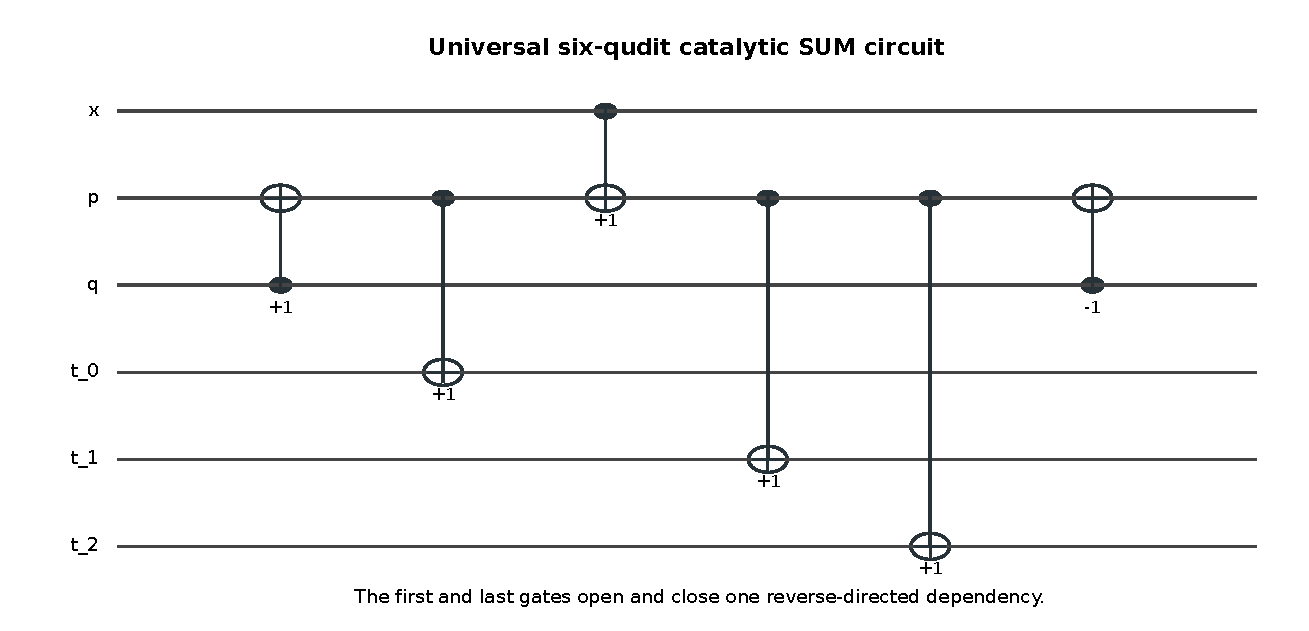
\includegraphics[width=.96\textwidth]{qudit_sum_circuit.pdf}
\caption{The universal six-qudit catalytic circuit.  Coefficients are interpreted modulo $d$.}
\label{fig:qudit-sum}
\end{figure}

A lower-only word needs seven gates.  The exact proof is coefficient-domain independent because it uses pivot support and the number of distinct carrier states rather than division.

\section{Connected higher-dimensional qudit families}
The snapshot target $A(u;s_1,\ldots,s_v)$ from the core chapter is defined over any coefficient ring for which the displayed additions make sense.  Over $\Z_d$, it becomes a modular SUM circuit.  Its explicit ambient word uses exactly two reverse-directed SUM gates and has length
\[
u+v+2.
\]
The interval-tree proof of exact restricted length is most transparent over fields, but the displayed upper-bound and resource-amortization mechanism remain valid over every $\Z_d$.

For a field $\F_q$, the exact formula is
\[
\ellDown(A)=u+2v,
\qquad
\ellAll(A)\le u+v+2,
\]
so
\[
\Delta(A)\ge v-2.
\]
The connected family has asymptotic ratio approaching $3/2$.

\section{Weighted physical costs}
Suppose forward SUM gates cost one and reverse-directed SUM gates cost $\lambda$.  The displayed word has weighted cost
\[
u+v+2\lambda,
\]
while the restricted construction costs $u+2v$.  Hence the gain is at least
\[
v-2\lambda.
\]
This formula can be combined with hardware calibration.  If reverse orientation requires echo pulses or routing, the catalyst remains useful when the number of exported snapshots exceeds twice the effective penalty.

\begin{boundarybox}
A gate-count saving does not imply a lower physical error or depth.  Device-specific conclusions require a cost vector containing duration, infidelity, crosstalk, and routing.  The algebraic theorem identifies candidate rewrites and the exact break-even inequality.
\end{boundarybox}

\section{Pauli action for prime qudits}
For odd prime $d$, let $X$ and $Z$ denote generalized Pauli operators.  The SUM gate acts by
\begin{align*}
X_s&\mapsto X_sX_t^a,
&
X_t&\mapsto X_t,\\
Z_s&\mapsto Z_s,
&
Z_t&\mapsto Z_s^{-a}Z_t.
\end{align*}
Thus the modular linear action embeds into a symplectic transformation.  The catalytic row excursion has a dual Pauli interpretation: a temporary reverse dependency changes both $X$ propagation and the contragredient $Z$ propagation, then restores them.

This makes the SUM family a bridge between the transvection paper and the Clifford chapter.  It is the only quantum extension in this monograph that follows directly from the ring-universal theorem without a new finite search.

\section{Continuous-variable shear analogue}
On continuous variables, a linear coordinate map $A$ embeds symplectically as
\[
A\longmapsto
\begin{pmatrix}
A&0\\
0&A^{-T}
\end{pmatrix}.
\]
A row shear therefore gives a Gaussian SUM transformation.  The six-row word identity remains a matrix identity in the corresponding shear subgroup.

\begin{skeletonbox}
To claim an advantage in a full Gaussian gate library, one must compare against rotations, squeezers, beam splitters, and general symplectic decompositions.  The current theorem proves a defect only inside the directed-shear versus all-shear comparison.
\end{skeletonbox}

\section{Compiler primitive}
A compiler can search for a carrier row $p$, a temporary source $q$, and output rows requiring several successive states of $p$.  The symbolic pattern is:
\begin{enumerate}
\item add $q$ into $p$ in the disallowed direction,
\item update $p$ through a sequence of allowed additions,
\item copy selected intermediate states of $p$ into outputs,
\item subtract $q$ from $p$,
\item verify that the outputs contain the intended modular combinations.
\end{enumerate}
The Python function \texttt{snapshot\_target} constructs the target and \texttt{snapshot\_ambient\_word} emits the word.

\begin{lstlisting}[style=pythonstyle,caption={Constructing a modular snapshot family.}]
from catalytic_gate_atlas.linear import (
    snapshot_target,
    snapshot_ambient_word,
    apply_row_word,
)

u = 4
phases = [0, 2, 4]
modulus = 5
A = snapshot_target(u, phases, modulus)
word = snapshot_ambient_word(u, phases, modulus)
assert apply_row_word(len(A), word, modulus) == A
\end{lstlisting}

\section{Open qudit questions}
\begin{question}
Does the first defective dimension remain six for every finite field and every modular ring $\Z_d$ under the directed-SUM metric?
\end{question}
\begin{question}
Can qudit Clifford gates outside the SUM subgroup produce a larger defect for a SUM target under total, entangling, or depth cost?
\end{question}
\begin{question}
Do composite dimensions admit characteristic-dependent catalytic motifs unavailable over fields?
\end{question}

\chapter{Catalytic basis escape in symplectic Clifford synthesis}\label{ch:clifford}
\index{Clifford group}
\index{symplectic group}
\index{parabolic subgroup}
\index{CSS circuit}
\index{entangling count}


\section{Binary symplectic representation}
Modulo global phase and Pauli translations, an $n$-qubit Clifford operation acts on Pauli exponent vectors
\[
v=(x_0,\ldots,x_{n-1}\mid z_0,\ldots,z_{n-1})^T\in\F_2^{2n}
\]
through a symplectic matrix
\[
M\in\Sp(2n,2).
\]
The elementary gates used here act as follows:
\begin{align*}
H_i &: (x_i,z_i)\mapsto(z_i,x_i),\\
S_i &: z_i\mapsto z_i+x_i,\\
\CX_{i\to j} &: x_j\mapsto x_j+x_i,
\quad z_i\mapsto z_i+z_j,\\
\CZ_{ij} &: z_i\mapsto z_i+x_j,
\quad z_j\mapsto z_j+x_i.
\end{align*}

Let $P_n\le\Sp(2n,2)$ be the parabolic subgroup stabilizing the $Z$ Lagrangian
\[
L_Z=\{(0\mid z):z\in\F_2^n\}.
\]
The gates $S$, $\CZ$, and $\CX$ preserve $L_Z$.  Hadamard gates do not.

\begin{definition}[Parabolic and ambient Clifford metrics]
The restricted alphabet is
\[
\mathcal S_P
=
\{S_i,\CZ_{ij},\CX_{i\to j}\},
\]
and the ambient alphabet is
\[
\mathcal S_C
=
\mathcal S_P\cup\{H_i\}.
\]
Targets lie in $P_n$.  We study both total primitive count and entangling count, where $H_i$ and $S_i$ have cost zero while $\CX$ and $\CZ$ have cost one.
\end{definition}

This is a precise basis-escape model.  It is not the unique meaning of ``CSS preserving'' or ``Clifford cost.''  It is chosen because both groups are finite and the restricted subgroup has a clean Lagrangian interpretation.

\section{Exact group sizes}
The finite state spaces are
\[
|P_n|
=
2^{n(n+1)/2}|\GL(n,2)|,
\]
and
\[
|\Sp(2n,2)|
=
2^{n^2}\prod_{j=1}^n(2^{2j}-1).
\]
For $n=1,2,3$ this gives:
\begin{center}
\begin{tabular}{@{}rcc@{}}
\toprule
$n$&$|P_n|$&$|\Sp(2n,2)|$\\
\midrule
1&2&6\\
2&48&720\\
3&10,752&1,451,520\\
\bottomrule
\end{tabular}
\end{center}
These sizes permit exhaustive breadth-first or zero-one search through three qubits.

\section{Total primitive count}
\begin{computedbox}
With every gate in $\mathcal S_P$ and $\mathcal S_C$ assigned unit cost and with SWAP excluded as a primitive, exhaustive search gives:
\begin{center}
\begin{tabular}{@{}rcccc@{}}
\toprule
$n$&restricted diameter&ambient diameter&defective targets&maximum defect\\
\midrule
1&1&3&0&0\\
2&5&8&0&0\\
3&8&12&24&1\\
\bottomrule
\end{tabular}
\end{center}
At $n=3$, six targets have distance pair $(7,6)$ and eighteen have pair $(8,7)$.
\end{computedbox}

Thus three qubits are the first total-count threshold in this exact swap-free model.

\subsection{A three-qubit witness}
One defective target has symplectic matrix
\[
M_3=
\begin{pmatrix}
0&1&0&0&0&0\\
0&0&1&0&0&0\\
1&0&0&0&0&0\\
1&0&1&0&1&0\\
0&1&0&0&0&1\\
0&1&0&1&0&0
\end{pmatrix}.
\]
A restricted word of length seven is
\[
\CX_{0\to2},
\CZ_{12},
\CX_{2\to0},
\CX_{0\to2},
\CX_{0\to1},
\CX_{1\to0},
\CX_{0\to1}.
\]
An ambient word of length six is
\[
H_1,
\CX_{1\to2},
\CX_{2\to1},
\CX_{2\to0},
\CX_{0\to2},
H_0.
\]

\begin{figure}[ht]
\centering
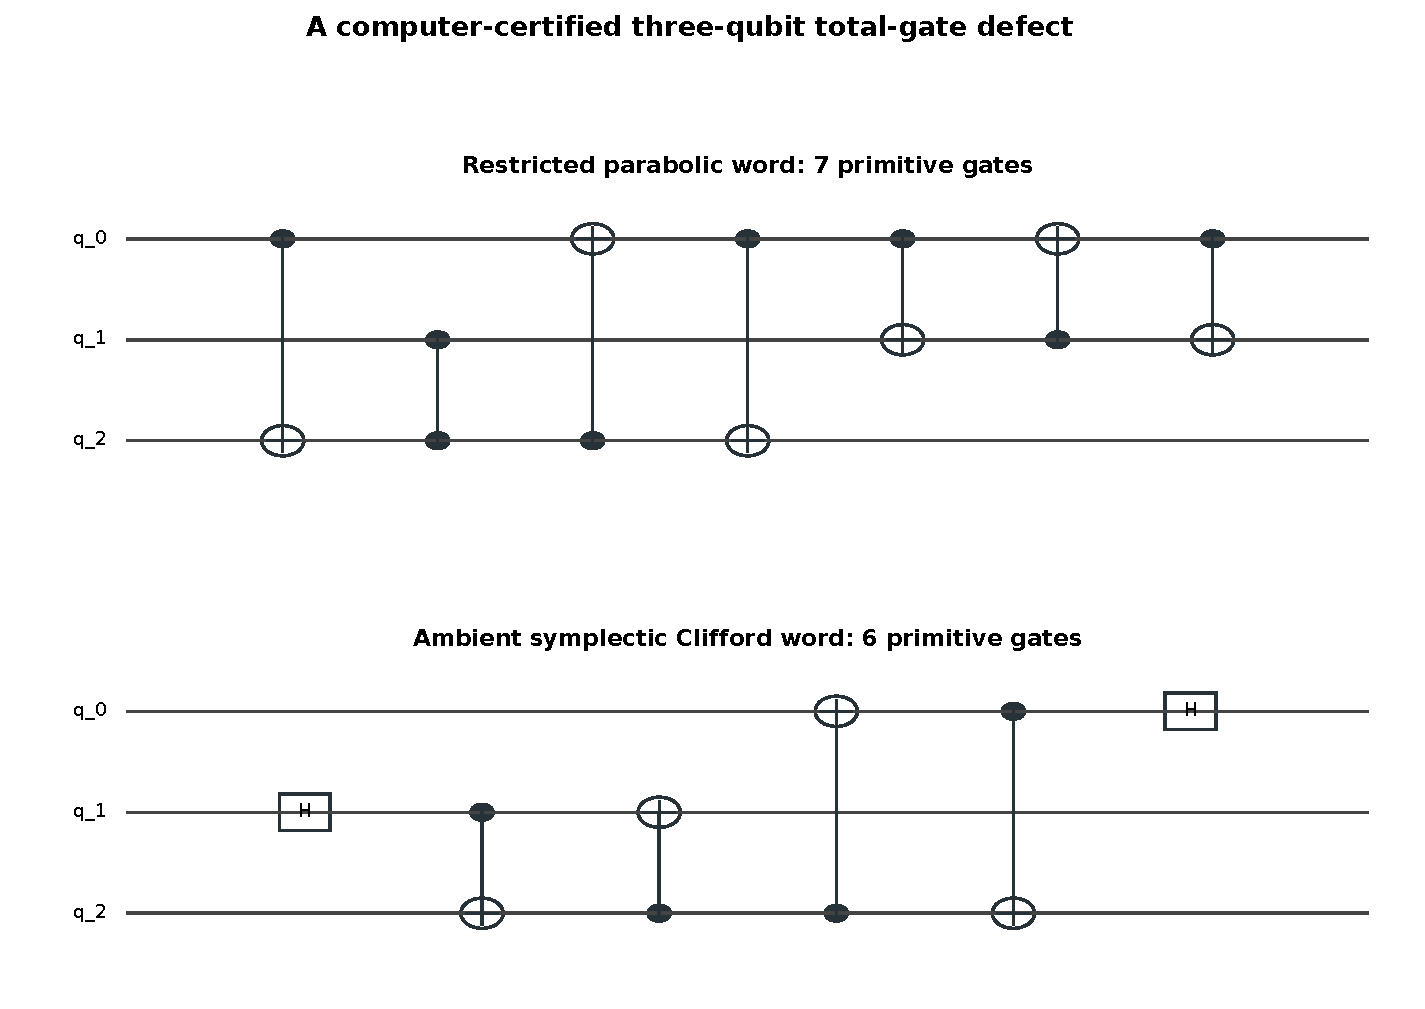
\includegraphics[width=.98\textwidth]{clifford_three_qubit_defect.pdf}
\caption{A swap-free three-qubit parabolic target with total primitive-count defect one.}
\label{fig:clifford-three}
\end{figure}

The Hadamards do not form a matched pair on the same wire.  They open and close the Lagrangian excursion in different coordinates.  This is a useful warning against assuming that every catalyst has the literal form $g\cdots g^{-1}$.

\section{SWAP sensitivity}
Add $\SWAP_{ij}$ to both alphabets as a unit-cost primitive.  The target groups remain unchanged, but the metric changes.

\begin{computedbox}
For $n=3$ with unit-cost SWAP gates, the restricted diameter drops from eight to seven, the ambient diameter drops from twelve to eleven, and every one of the $10,752$ parabolic targets has zero total-count defect.
\end{computedbox}

The preceding twenty-four defects therefore measure a real gate-alphabet distinction, not an invariant of the subgroup inclusion alone.  In many architectures SWAP is not elementary and costs three CNOTs, while in others qubit movement or relabeling changes the accounting.  The theorem must retain the convention.

\section{Entangling-count defects}
Now assign cost zero to $H_i$ and $S_i$ and cost one to $\CX$ and $\CZ$.

\begin{computedbox}
The exact censuses are:
\begin{center}
\begin{tabular}{@{}rccc@{}}
\toprule
$n$&defective targets&distance pairs&maximum defect\\
\midrule
1&0&none&0\\
2&4&$(3,2)$ with multiplicity $4$&1\\
3&1,624&
$\begin{array}{c}
(3,2):24,\ (4,3):432,\ (5,4):1056,\\
(6,4):48,\ (6,5):64
\end{array}$
&2\\
\bottomrule
\end{tabular}
\end{center}
\end{computedbox}
The entangling metric has an earlier threshold and a larger exceptional set.

\subsection{A two-qubit witness}
A canonical target is
\[
M_2=
\begin{pmatrix}
0&1&0&0\\
1&0&0&0\\
1&1&0&1\\
1&1&1&0
\end{pmatrix}.
\]
A restricted realization is
\[
\CX_{0\to1},
S_1,
\CX_{1\to0},
\CX_{0\to1},
\]
with three entangling gates.  An ambient realization is
\[
H_1,
\CX_{1\to0},
\CX_{0\to1},
H_0,
S_1,
S_0,
\]
with two entangling gates.

\begin{figure}[ht]
\centering
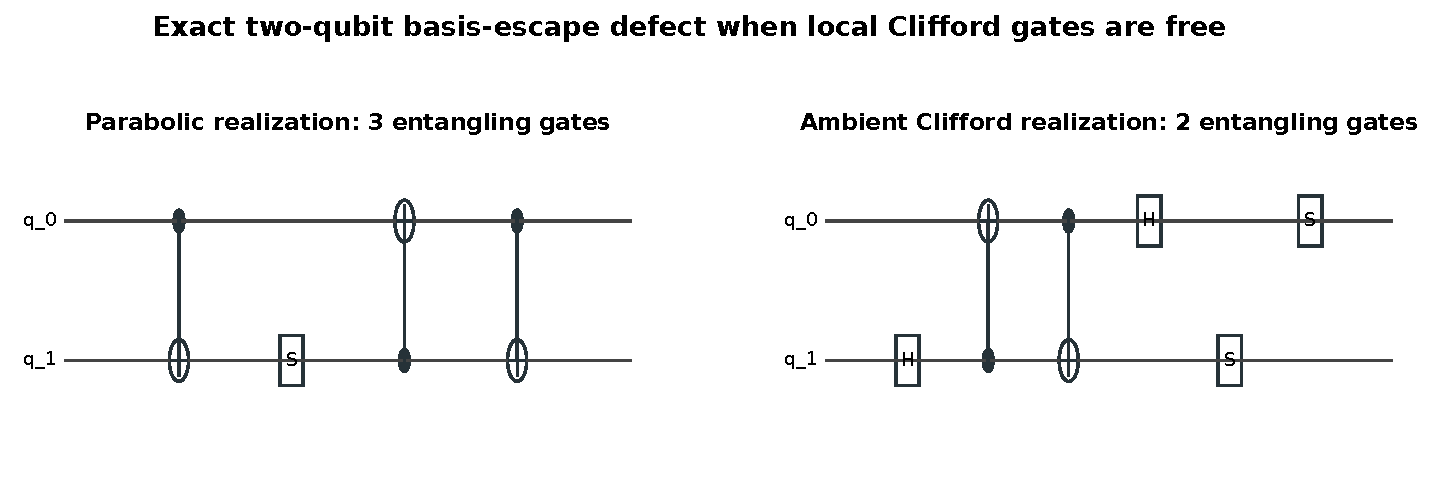
\includegraphics[width=.98\textwidth]{clifford_two_qubit_defect.pdf}
\caption{A two-qubit entangling-count defect.  Local Clifford gates are free in this cost model.}
\label{fig:clifford-two}
\end{figure}

\section{Census summary}
\subsection{An analytic certificate for the four two-qubit defects}

The four exceptional matrices admit one common lower-bound proof.  Work in the declared symplectic quotient and entangling metric, with $H_i$ and $S_i$ free and SWAP excluded as a primitive.  Put
\[
J_2=\begin{pmatrix}0&1\\1&0\end{pmatrix},
\qquad D=\operatorname{diag}(d_0,d_1),
\qquad d_0,d_1\in\F_2,
\]
and define
\[
M_D=\begin{pmatrix}J_2&0\\I_2+DJ_2&J_2\end{pmatrix}.
\]

\begin{theorem}[Two-qubit orbit and exact costs]\label{thm:clifford-two-analytic}
Each of the four distinct matrices $M_D$ lies in $P_2$ and has restricted entangling cost three and ambient entangling cost two.  They form one orbit under left multiplication by the free restricted subgroup generated by $S_0,S_1$.
\end{theorem}
\begin{proof}
The ambient sequence
\[
H_1,\ \CX_{1\to0},\ \CX_{0\to1},\ H_0
\]
has matrix $M_0=\left(\begin{smallmatrix}J_2&0\\I_2&J_2\end{smallmatrix}\right)$.  Applying $S_0^{d_0}S_1^{d_1}$ afterwards left multiplies by $\left(\begin{smallmatrix}I_2&0\\D&I_2\end{smallmatrix}\right)$ and gives $M_D$.  These matrices are distinct because $J_2$ is invertible.  This also proves their orbit statement and the ambient upper bound two.  The displayed restricted sequence for $M_2$ above gives $M_{I_2}$ using three CNOT gates and one free $S_1$.  Free final phase gates then give every $M_D$, proving the restricted upper bound three.

For the restricted lower bound, the upper-left block of a parabolic product is the product of its upper-left blocks.  Each $S$ or CZ contributes $I_2$, while the two directed CNOTs contribute the elementary matrices
\[
L=\begin{pmatrix}1&0\\1&1\end{pmatrix},
\qquad U=\begin{pmatrix}1&1\\0&1\end{pmatrix}.
\]
Products using at most two CNOTs belong to $\{I_2,L,U,LU,UL\}$, which does not contain $J_2$.  Thus any restricted circuit for $M_D$ requires at least three charged gates.

For the ambient lower bound, reorder the coordinates as $(x_0,z_0\mid x_1,z_1)$.  A local Clifford acts by an invertible block-diagonal matrix in this order.  In $M_D$, each of the two diagonal $2\times2$ blocks is $\left(\begin{smallmatrix}0&0\\1&0\end{smallmatrix}\right)$ and has rank one.  In either directed CNOT or CZ, both diagonal blocks are $I_2$ and have rank two.  Left and right multiplication by local Cliffords preserve these diagonal-block ranks.  A circuit with one charged gate has the form $K_1 E K_2$ with $K_1,K_2$ local and $E$ a CNOT or CZ, so it cannot equal $M_D$.  A circuit with no charged gate is local and also has rank-two diagonal blocks.  The ambient cost is therefore at least two.
\end{proof}

The complete finite census finds exactly four defective targets.  Since the theorem supplies four distinct defective targets, it identifies the entire exceptional set in that census.  The exact costs and orbit description above have analytic proofs, while completeness of the finite classification retains the exhaustive-search evidence.

\begin{figure}[ht]
\centering
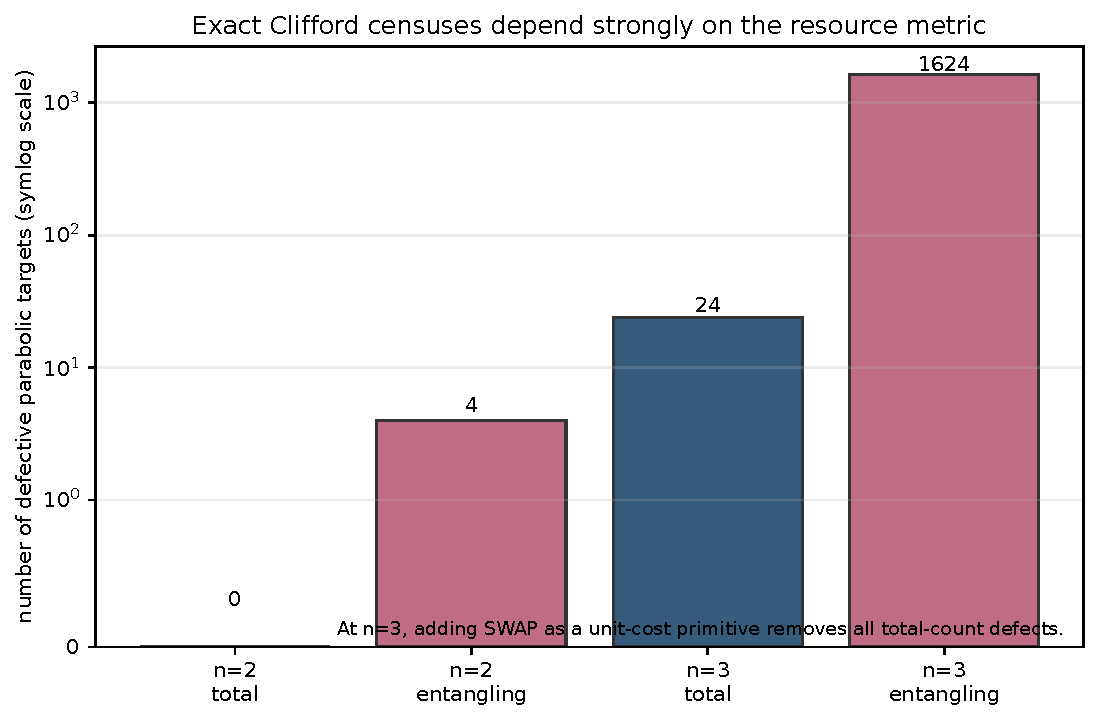
\includegraphics[width=.76\textwidth]{clifford_census.pdf}
\caption{Exact parabolic-versus-ambient Clifford census.  The vertical scale is symlogarithmic.}
\label{fig:clifford-census}
\end{figure}

The results establish three distinct lessons.
\begin{enumerate}
\item Basis escape produces genuine Clifford defects, not only linear CNOT defects.
\item The first threshold depends on whether local gates are free.
\item Adding a SWAP primitive can eliminate a finite total-count threshold.
\end{enumerate}

\section{Search completeness}
The search state is the exact $2n\times2n$ binary symplectic matrix.  Every generator acts by a fixed row update.  Ordinary breadth-first search gives exact unit-cost distances.  Zero-one breadth-first search gives exact entangling costs.  Since every state of $P_n$ and $\Sp(2n,2)$ is reached, comparing the two distance maps is a complete census.

The optimized C++ verifier represents a $6\times6$ matrix by a $36$-bit integer.  It enumerates the full three-qubit group in a few seconds in the present environment.  The Python implementation is slower but independently expresses the same state model.

\section{Interpretation as symplectic holonomy}
The parabolic subgroup is a fiber over the Lagrangian Grassmannian.  A Hadamard moves one coordinate out of the chosen Lagrangian.  The ambient path traverses other Lagrangian frames and returns to a target stabilizing $L_Z$.

This is the symplectic analogue of the unitriangular Schreier loop.  The catalyst is a temporary exchange of $X$ and $Z$ roles.  The consumers are entangling gates that become cheaper in the changed frame.

\section{CSS-preserving extensions}
The parabolic model fixes one Lagrangian, but CSS circuit classes can be defined more narrowly or more broadly.  Possible restricted alphabets include:
\begin{enumerate}
\item CNOT and Pauli gates only,
\item CNOT, $S$, and diagonal controlled phases,
\item block-diagonal symplectic transformations preserving separate $X$ and $Z$ codes,
\item logical Clifford gates preserving a CSS stabilizer decomposition,
\item architecture-constrained versions of the preceding models.
\end{enumerate}
Each produces a different subgroup and metric.

\begin{skeletonbox}
A full CSS threshold paper should classify cost-preserving orbits of minimal defects, identify a symplectic-flag lower-bound invariant, and determine which defects survive when SWAP, qubit permutation, or local Cliffords are assigned alternative costs.
\end{skeletonbox}

\section{Depth and parallelism}
Gate-count defects do not automatically imply depth defects.  Given a gate sequence, define its dependency graph and schedule commuting or disjoint gates in parallel.  The appropriate quantities are
\[
\Delta_{\mathrm{depth}}(U),
\qquad
\Delta_{\mathrm{2q-depth}}(U),
\qquad
\Delta_{\mathrm{space-time}}(U).
\]
A basis change applied transversally to many qubits may have small depth even when its total count is large.  Conversely, a two-gate count saving can increase depth under locality constraints.

\section{Open Clifford problems}
\begin{question}
What are the defect orbits of the twenty-four three-qubit total-count targets under qubit permutations and parabolic conjugation?
\end{question}
\begin{question}
Does the maximum parabolic-versus-Clifford defect grow linearly, as $n\log n$, or faster under total primitive count?
\end{question}
\begin{question}
Can one prove a symbolic family with entangling-count defect greater than two, rather than relying on finite census data?
\end{question}
\begin{question}
Which finite symplectic parabolics are geodesically convex after SWAP is included as a primitive?
\end{question}
\begin{conjecturebox}
The observed three-qubit defects should admit a small collection of symplectic root motifs analogous to the three-cross, one-phase classification in the unitriangular case.  The present monograph records the exact census and witnesses but does not claim that classification.
\end{conjecturebox}

\chapter{Temporary nonlinearity: affine logic versus Toffoli-assisted synthesis}\label{ch:affine-toffoli}
\index{Toffoli gate}
\index{affine reversible circuit}
\index{temporary nonlinearity}
\index{algebraic normal form}


\section{The question}
Let
\[
\operatorname{AGL}(n,2)
=
\{x\mapsto Ax+b:A\in\GL(n,2),\ b\in\F_2^n\}
\]
be the affine reversible group.  It is generated by NOT and CNOT gates.  The ambient gate set adds Toffoli.  On three bits it generates the full reversible group.  On $n\ge4$ bits with no ancillas, each NOT, CNOT, or Toffoli gate is an even permutation, so this alphabet does not generate the full symmetric group.

The catalytic question is:
\begin{quote}
Can a circuit temporarily create nonlinear Boolean terms with Toffoli gates, reuse them, cancel them completely, and implement a final affine permutation with fewer gates than every affine circuit?
\end{quote}
This is the nonlinear analogue of dirty linear memory.

\section{Algebraic normal form}
Every Boolean coordinate function has a unique algebraic normal form
\[
f_i(x)
=
\bigoplus_{S\subseteq[n]}a_{i,S}\prod_{j\in S}x_j.
\]
Affine maps have degree at most one.  A Toffoli gate targeting $t$ with controls $a,b$ performs
\[
x_t\longmapsto x_t+x_ax_b,
\]
which can raise the degree of later coordinates.  The final affine target requires every higher-degree coefficient to cancel.

A candidate lower-bound invariant must do more than track maximum degree.  One Toffoli creates degree two and a second can remove it.  Useful refinements include:
\begin{itemize}
\item the dimension of the quadratic monomial span,
\item directional derivatives $D_u f(x)=f(x+u)+f(x)$,
\item the rank of the bilinear polarization,
\item the number of outputs consuming a nonlinear workspace term,
\item restoration obligations for every nonlinear carrier.
\end{itemize}

\section{Exact three-bit census}
On three bits,
\[
|\operatorname{AGL}(3,2)|
=2^3|\GL(3,2)|
=1344,
\]
while the group generated by NOT, CNOT, and Toffoli is the full permutation group
\[
S_8,
\qquad |S_8|=40320.
\]
Both spaces can be enumerated exactly.

\begin{computedbox}
For three bits, every affine target has the same minimum cost in the affine gate set and in the Toffoli-assisted gate set under each of the following metrics:
\begin{enumerate}
\item total primitive gate count, where NOT, CNOT, and Toffoli cost one,
\item entangling count, where NOT is free and CNOT and Toffoli cost one.
\end{enumerate}
There are no defective affine targets among all $1344$ targets.
\end{computedbox}

The restricted total-count diameter is seven and the ambient diameter on $S_8$ is eight.  Under entangling count, both relevant diameters are six.  Equality on affine targets is stronger than a diameter comparison because every target is checked individually.

\begin{figure}[ht]
\centering
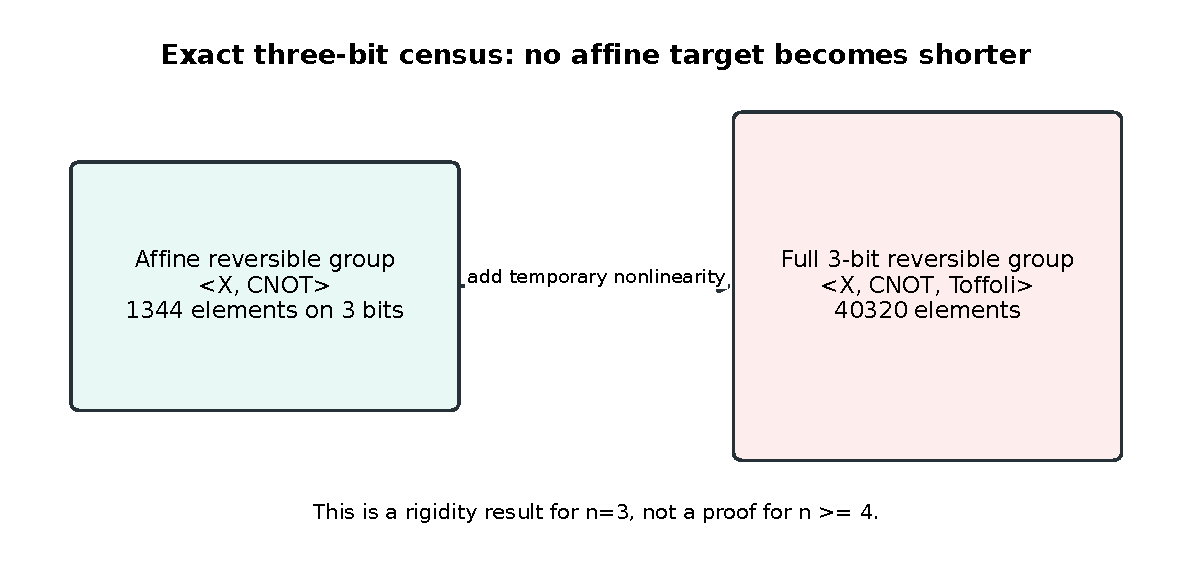
\includegraphics[width=.84\textwidth]{affine_toffoli_census.pdf}
\caption{The complete three-bit affine-versus-Toffoli census is rigid.}
\label{fig:affine-toffoli-census}
\end{figure}

\section{Interpretation of the negative result}
The census does not show that temporary nonlinearity is useless in general.  It shows that three bits do not provide enough state space for a nonlinear carrier to repay its creation and cancellation cost under the stated alphabets.

The negative result is valuable for three reasons.
\begin{enumerate}
\item It gives a certified lower threshold: any total- or entangling-count defect requires at least four bits.
\item It prevents a forced analogy with the six-wire linear catalyst.
\item It supplies a complete regression test for future synthesis code.
\end{enumerate}

\section{A formal nonlinear catalyst}
A clean one-workspace template is
\[
T\;h_m\cdots h_1\;T^{-1},
\]
where $T$ is Toffoli and the middle gates use the quadratic term created in the workspace.  Since Toffoli is self-inverse, the displayed circuit uses two nonlinear gates.

\begin{figure}[ht]
\centering
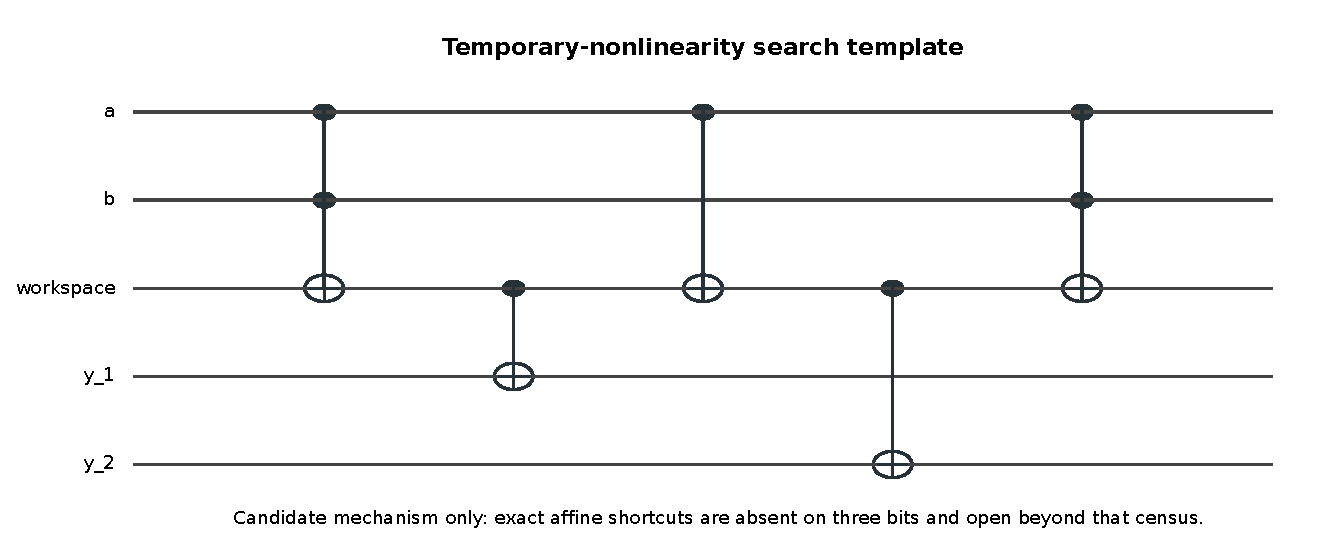
\includegraphics[width=.96\textwidth]{temporary_nonlinearity_skeleton.pdf}
\caption{A temporary-nonlinearity template.  It is a search skeleton, not a proved shortcut.}
\label{fig:nonlinear-skeleton}
\end{figure}

The key difficulty is that a final affine map cannot retain any product term.  Every output that consumed the nonlinear carrier must be repaired, or the nonlinear contributions must cancel collectively.

\section{Conjugation formulas}
Let $T_{ab\to t}$ denote Toffoli.  Conjugating an affine gate by $T$ can produce nonlinear permutations.  For example, if $X_t$ flips the target,
\[
T_{ab\to t}X_tT_{ab\to t}=X_t,
\]
so no gain occurs.  If a CNOT changes a control or exports the target, the conjugated map can contain several quadratic terms.  The exact formula is easiest in algebraic normal form: substitute the Toffoli-updated coordinate into the affine map, then apply the inverse substitution.

A systematic search should classify pairs $(T,h)$ for which
\[
ThT^{-1}\in\operatorname{AGL}(n,2).
\]
For one Toffoli and an affine middle word, this is a normalizer-intersection problem.  A useful next bounded test is to examine simple two-Toffoli sandwiches with an affine middle word of restricted length at most five.  The present archive contains no reproducible implementation or receipt for this four-bit test, so no negative result from it is claimed here.

\section{Potential lower-bound invariants}
\subsection{Quadratic support debt}
Let $Q(f)$ be the span of quadratic monomials appearing across the coordinate functions.  A Toffoli changes $Q(f)$ by at most a controlled rank-one contribution before subsequent substitutions.  If several outputs consume the same quadratic term, a dynamic debt invariant may charge its creation, distribution, and cancellation.

\subsection{Derivative rank}
For an affine map, every derivative $D_u f$ is constant.  During a nonlinear excursion, the derivative map
\[
u\mapsto D_u f(x)
\]
can depend on $x$.  One can track the dimension of the nonconstant derivative space and require it to return to zero.

\subsection{Higher-order Möbius coefficients}
The ANF coefficients are the Möbius transform of the truth table.  Projectors onto degree layers give an exact packet decomposition
\[
f=f^{(0)}+f^{(1)}+f^{(2)}+\cdots.
\]
A restricted affine circuit remains in degrees zero and one.  The ambient circuit can populate higher packets temporarily.  A successful lower bound must charge the useful flow through those packets, not merely their instantaneous dimension.

\section{Four-bit search architecture}
The full permutation group on four-bit states has size $16!$.  The declared no-ancilla gate alphabet lies in its alternating subgroup: NOT, CNOT, and Toffoli are respectively products of eight, four, and two disjoint transpositions.  Even this reduced ambient search is large enough to require a more structured approach.  Several exact approaches remain available.
\begin{enumerate}
\item Meet in the middle for a fixed candidate target and length.
\item SAT or SMT encoding of a length-$L$ circuit with affine endpoint constraints.
\item Bidirectional search restricted to states within a bounded nonlinear-degree or Toffoli-count budget.
\item Enumeration of two- or four-Toffoli normal forms modulo affine conjugation.
\item Mixed-integer or algebraic solving of ANF coefficient equations.
\end{enumerate}

\begin{protocol}[First four-bit threshold search]
\begin{enumerate}
\item Compute exact affine distances for all $322{,}560$ affine targets.
\item Enumerate ambient words with two Toffoli gates modulo affine gates on the left and right.
\item Retain words whose endpoint is affine.
\item Compare with the exact affine distance.
\item If no defect appears, increase the Toffoli budget and produce an unsatisfiability certificate for every shorter length.
\end{enumerate}
\end{protocol}
This protocol is a research plan.  The packaged executable census stops at three bits, and neither the four-bit normal-form search nor its lower-bound certificates is supplied.

\section{Resource variants}
Temporary nonlinearity may be useful under one metric and useless under another.  Natural costs include:
\[
\begin{gathered}
\text{Toffoli count},\quad \text{CNOT count},\quad
T\text{-count after decomposition},\quad T\text{-depth},\\
\text{ancilla count},\quad \text{total depth}.
\end{gathered}
\]
A Toffoli-assisted affine shortcut in total Boolean gates might disappear after fault-tolerant decomposition.  Conversely, a circuit with more Boolean primitives can reduce $T$-depth.

\section{Related nonlinear gate families}
The same program applies to:
\begin{itemize}
\item CCZ-assisted diagonal Boolean phase maps,
\item relative-phase Toffoli gates,
\item multi-controlled $X$ and $Z$ gates,
\item Reed--Muller degree hierarchies,
\item reversible arithmetic over $\Z_d$,
\item polynomial automorphisms over finite rings.
\end{itemize}

\begin{conjecturebox}
There exists an affine target on finitely many bits whose total or fault-tolerant resource cost is reduced by a restored nonlinear excursion.  The exact three-bit census rules out the smallest possible instance but supplies no evidence for a particular larger threshold.
\end{conjecturebox}

\section{Reproducible code}
The implementation represents every reversible map as an exact permutation of $2^n$ basis states.  Breadth-first search enumerates both the affine group and the full three-bit reversible group.

\begin{lstlisting}[style=pythonstyle,caption={Exact three-bit affine-versus-Toffoli census.}]
from catalytic_gate_atlas import exact_affine_toffoli_census

print(exact_affine_toffoli_census(3, entangling_cost=False))
print(exact_affine_toffoli_census(3, entangling_cost=True))
\end{lstlisting}
The expected defect count is zero in both outputs.

\chapter{Phase-polynomial and Clifford+\texorpdfstring{$T$}{T} catalysis}\label{ch:phase-cliffordt}
\index{Clifford+T circuit}
\index{phase polynomial}
\index{T-count}
\index{T-depth}
\index{Pareto defect}


\section{Why the phase setting is different}
Fault-tolerant quantum compilation rarely assigns equal cost to every gate.  Clifford operations are often treated as inexpensive relative to non-Clifford gates, while connectivity and parity computation can dominate the remaining cost.  Consequently there is no single Clifford+$T$ defect.  One must specify at least
\[
\mathbf c(U)=
\bigl(
T\text{-count},
T\text{-depth},
\text{two-qubit count},
\text{two-qubit depth},
\text{ancillas}
\bigr).
\]
A catalytic excursion may improve one component and worsen another.  The natural comparison is therefore Pareto-valued rather than scalar unless a hardware-specific weight vector is fixed.

Let $\omega=e^{i\pi/4}$.  A phase-polynomial circuit on $n$ qubits has the form \cite{AmyMosca2019,Selinger2013}
\begin{equation}\label{eq:phase-poly-normal}
U\ket{x}=\omega^{P(x)}\ket{Ax+b},
\end{equation}
where $A\in\GL(n,2)$, $b\in\F_2^n$, and $P:\F_2^n\to\Z_8$ is represented as a sum of binary linear forms with coefficients in $\Z_8$.  The diagonal case has $A=I$ and $b=0$.

The restricted model may be chosen in several ways:
\begin{enumerate}
\item diagonal phase gadgets only;
\item CNOT-dihedral circuits generated by $X$, CNOT, and $T$;
\item parity networks in which every intermediate transformation remains affine on computational basis labels;
\item a prescribed family of commuting Pauli rotations.
\end{enumerate}
The ambient model may add Hadamards, arbitrary Clifford conjugations, measurements, or ancillas.  These choices define different problems.

\section{Pauli-rotation language}
For a Pauli operator $P$ and angle $\theta$, write
\[
R_P(\theta)=e^{-i\theta P/2}.
\]
Every Clifford $C$ satisfies
\begin{equation}\label{eq:pauli-conjugation}
C R_P(\theta) C^\dagger=R_{CPC^\dagger}(\theta).
\end{equation}
Thus a short ambient basis change can rotate a large family of phase gadgets into a different commuting or nearly commuting family, apply them there, and rotate back.

\begin{provedbox}
Equation \eqref{eq:pauli-conjugation} is an exact catalytic transport identity.  It does not by itself prove a gate-count defect.  A defect additionally requires a lower bound showing that the transported family is more expensive in the restricted representation than the opening and closing Clifford layers plus the transported implementation.
\end{provedbox}

The simplest symbolic sandwich is
\[
C\left(\prod_{j=1}^m R_{P_j}(\theta_j)\right)C^\dagger
=
\prod_{j=1}^m R_{CP_jC^\dagger}(\theta_j).
\]
If the $P_j$ commute, their conjugates commute.  A catalyst can therefore change the geometry of the support without changing the algebra of the angles.

\section{Phase polynomials and parity carriers}
A CNOT network computes linear parities
\[
\lambda(x)=a\cdot x\in\F_2.
\]
Applying $T^k$ to a wire carrying $\lambda(x)$ contributes
\[
\omega^{k\lambda(x)}
\]
to the phase polynomial.  A parity network must create each required parity, expose it to a phase gate, and restore the linear map required at the endpoint.

This makes phase-polynomial synthesis a close relative of the snapshot families in the linear core.  A parity row may evolve through
\[
\lambda_0,\lambda_1,\ldots,\lambda_m,
\]
with selected states consumed by phase gates.  The difference is that consumption need not copy the parity to another row; it can deposit phase while leaving the carrier unchanged.

\begin{skeletonbox}
A candidate phase catalyst consists of:
\begin{enumerate}
\item a Clifford $C$ that opens a non-diagonal frame;
\item an evolving Pauli or parity carrier in that frame;
\item several phase rotations consuming intermediate carrier states;
\item $C^\dagger$ restoring the original diagonal or CNOT-dihedral model;
\item a certificate that no restricted parity network attains the same resource vector.
\end{enumerate}
\end{skeletonbox}

\begin{figure}[ht]
\centering
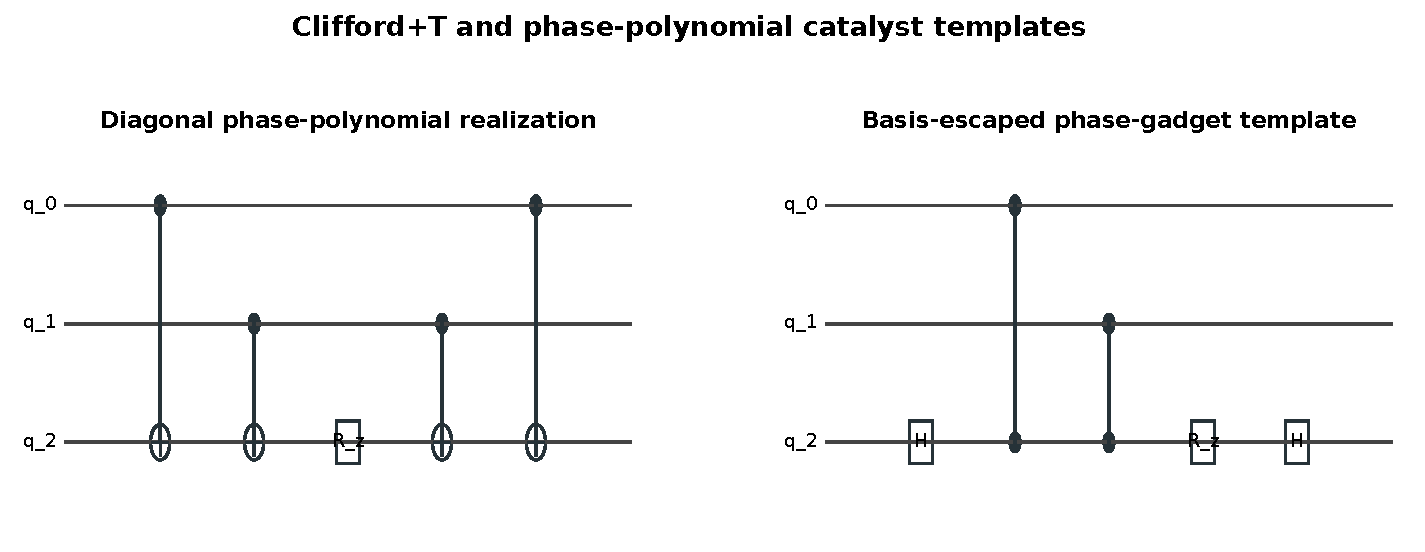
\includegraphics[width=.94\textwidth]{phase_polynomial_skeleton.pdf}
\caption{Symbolic Clifford+$T$ catalyst: a basis excursion transports a family of phase obligations and is removed at the endpoint.}
\label{fig:phase-polynomial-skeleton}
\end{figure}

\section{\texorpdfstring{$T$}{T}-count as a coding problem}
For diagonal Clifford+$T$ synthesis without ancillas, equivalent phase-polynomial descriptions can differ by identities whose coefficients vanish modulo eight on Boolean inputs.  Minimizing the number of odd coefficients is naturally expressed as a coset-decoding problem in a punctured Reed--Muller-type code.

Let $a\in\Z_8^{2^n-1}$ index nonzero linear forms and let $\operatorname{odd}(a)$ denote the binary vector recording which coefficients are odd.  An abstract restricted $T$-count is
\[
\ell_T(P)=
\min_{a:\,P_a=P}
\operatorname{wt}(\operatorname{odd}(a)).
\]
An ambient Clifford excursion changes not only the coefficient vector but also the Pauli frame in which the rotations are represented.  A lower bound that survives ambient Clifford conjugation must therefore be invariant under the relevant symplectic action or must explicitly charge the frame change.

\section{\texorpdfstring{$T$}{T}-depth and commuting layers}
Two phase gadgets may share a $T$ layer when a suitable Clifford network maps their parities to distinct wires or when ancilla resources permit parallel extraction.  Define the conflict graph $\Gamma_P$ whose vertices are odd phase terms and whose edges encode inability to realize two terms in one layer under the chosen ancilla and connectivity rules.  Then
\[
T\text{-depth}(P)\ge\chi(\Gamma_P)
\]
for any conflict graph whose edge relation is sound.  Catalysis can alter $\Gamma_P$ by changing the Pauli frame.  The right question is not merely whether $C$ preserves the number of terms, but whether it reduces the chromatic or scheduling obstruction enough to repay its own depth.

\section{A vector-valued defect}
For a target $U$ in a restricted phase model, define
\[
\mathcal C_{\mathrm{res}}(U)
=
\{\mathbf c(\mathcal W):\mathcal W\text{ is a restricted circuit for }U\}
\]
and similarly $\mathcal C_{\mathrm{amb}}(U)$.  Their Pareto frontiers are denoted $\operatorname{Pareto}_{\mathrm{res}}(U)$ and $\operatorname{Pareto}_{\mathrm{amb}}(U)$.

\begin{definition}[Pareto catalytic defect]
A target has a Pareto catalytic defect when the ambient Pareto frontier contains a point strictly dominating every restricted cost vector in at least one declared region of resource space.
\end{definition}

Scalarization by positive weights $w$ gives
\[
\Delta_w(U)=
\min_{c\in\mathcal C_{\mathrm{res}}(U)}w\cdot c
-
\min_{c\in\mathcal C_{\mathrm{amb}}(U)}w\cdot c.
\]
Different $w$ can change the magnitude of the defect and whether it is zero or positive.  It remains nonnegative because every restricted realization is also an ambient realization with the same resource vector.

\section{Exact finite-search model}
A finite exact atlas can be built \cite{KliuchnikovEtAl2013,AmyEtAl2013} for small $n$ by representing Clifford+$T$ operators in one of three ways.
\begin{enumerate}
\item Exact matrices over the cyclotomic ring $\Z[1/\sqrt2,i]$ modulo global phase.
\item Normal forms combining a binary symplectic Clifford with a phase-polynomial record.
\item Quotients by left and right Clifford actions when only $T$-count is charged.
\end{enumerate}
The third model can be dramatically smaller but requires care: quotienting is sound only when the free Clifford actions in the cost model agree with the quotient relation.

\begin{protocol}[Small-width Clifford+$T$ threshold atlas]
\begin{enumerate}
\item Fix exact versus approximate synthesis, ancilla rules, and the resource vector.
\item Enumerate the restricted target subgroup or a complete set of normal forms.
\item Compute restricted Pareto frontiers by multiobjective shortest path.
\item Enumerate ambient states or use meet in the middle for candidate targets.
\item Store an optimal witness and a lower-bound certificate for every defect.
\item Classify defects under qubit permutation and free Clifford equivalence.
\end{enumerate}
\end{protocol}

\section{Lower-bound candidates}
\subsection{Odd-support rank}
The span of odd phase terms is invariant under some restricted rewrites but transforms covariantly under linear changes of variables.  Its dimension gives a coarse obstruction.

\subsection{Pauli support geometry}
Represent a commuting Pauli family by an isotropic subspace of $\F_2^{2n}$.  Restricted diagonal circuits remain in the $Z$ Lagrangian.  Ambient Clifford circuits move through the symplectic Grassmannian.  Distance from the $Z$ Lagrangian, together with the number of deposited rotations, is the phase analogue of microscopic flag escape.

\subsection{Moment and derivative packets}
For a phase function $P$, finite differences
\[
D_uP(x)=P(x+u)-P(x)\pmod8
\]
separate affine, quadratic, and higher interactions.  A hierarchy of derivative tensors can record temporary flow into nonlinear phase packets.

\subsection{Architecture-aware parity rank}
On a coupling graph, each parity has a Steiner cost.  A catalyst can be profitable by making several required parities share a Steiner tree.  A sound lower bound may combine cut rank with edge congestion and restoration debt.

\section{Tensor and repeated-module questions}
For targets $U$ and $V$, independent synthesis gives
\[
\ell_T(U\otimes V)
\le
\ell_T(U)+\ell_T(V)
\]
when the systems are disjoint and local Clifford cost is ignored.  Joint synthesis may be better because phase identities can couple terms across modules.  This motivates a stable regularization
\[
\tau_T(U)=
\liminf_{r\to\infty}
\frac{\ell_T(U^{\otimes r})}{r}.
\]
A one-copy rigid phase target could still display tensor activation.

\begin{conjecturebox}
There are diagonal or CNOT-dihedral targets whose Pareto frontier is strictly improved by a restored non-diagonal Clifford excursion.  The smallest qubit threshold and the resource component in which the first defect appears are open in this monograph.
\end{conjecturebox}

\section{What would count as a theorem}
A publishable first result in this direction should contain all of the following:
\begin{enumerate}
\item an exact target family and gate alphabets;
\item explicit ambient circuits;
\item a restricted lower bound for the same declared cost;
\item exact treatment of global phase and ancillas;
\item classification below the first threshold or a proof of minimality;
\item reproducible symbolic code.
\end{enumerate}
Merely rewriting a phase gadget with Hadamards is not sufficient.  The decisive content is the optimality comparison.

\chapter{Gaussian, matchgate, and fermionic catalytic models}\label{ch:gaussian}
\index{Gaussian circuit}
\index{matchgate}
\index{Bogoliubov transformation}
\index{fermionic Gaussian circuit}
\index{symplectic embedding}


\section{Two Gaussian settings}
Quantum Gaussianity occurs \cite{WeedbrookEtAl2012} in two closely related but algebraically different settings.

For $n$ bosonic modes, a Gaussian unitary acts on quadratures
\[
\mathbf r=(q_1,\ldots,q_n,p_1,\ldots,p_n)^T
\]
by an affine symplectic transformation
\[
\mathbf r\longmapsto S\mathbf r+d,
\qquad
S\in\Sp(2n,\R).
\]
For $n$ fermionic modes, a fermionic Gaussian unitary acts on $2n$ Majorana operators by
\[
\gamma\longmapsto O\gamma,
\qquad O\in SO(2n).
\]
Nearest-neighbor matchgates give a circuit presentation of a fermionic Gaussian subgroup on qubits.

In both cases one can choose a restricted subgroup preserving a flag, mode ordering, particle number, or bipartition, and compare it with a larger Gaussian or non-Gaussian gate set.

\section{An inherited symplectic shear theorem}
Every invertible linear transformation $A\in\GL(n,R)$ has a canonical symplectic embedding
\begin{equation}\label{eq:symplectic-embedding}
\iota(A)=
\begin{pmatrix}
A&0\\
0&A^{-T}
\end{pmatrix}.
\end{equation}
Indeed, with
\[
J=
\begin{pmatrix}0&I\\-I&0\end{pmatrix},
\]
one checks
\[
\iota(A)^T J\iota(A)=J.
\]
Thus every row-transvection identity in the established linear theory induces an exact identity between symplectic shear circuits.

\begin{provedbox}
Under a Gaussian gate alphabet in which each embedded elementary transvection $\iota(I+aE_{ij})$ is one primitive and direction is the only restriction, the universal six-row catalytic atom embeds into a twelve-quadrature Gaussian atom with restricted length seven and ambient length six.
\end{provedbox}

This is a formal inheritance statement for the declared shear alphabet.  It does not assert optimality after arbitrary beam splitters, squeezers, Fourier transforms, or local Gaussian gates are admitted at unit cost.

\begin{figure}[ht]
\centering
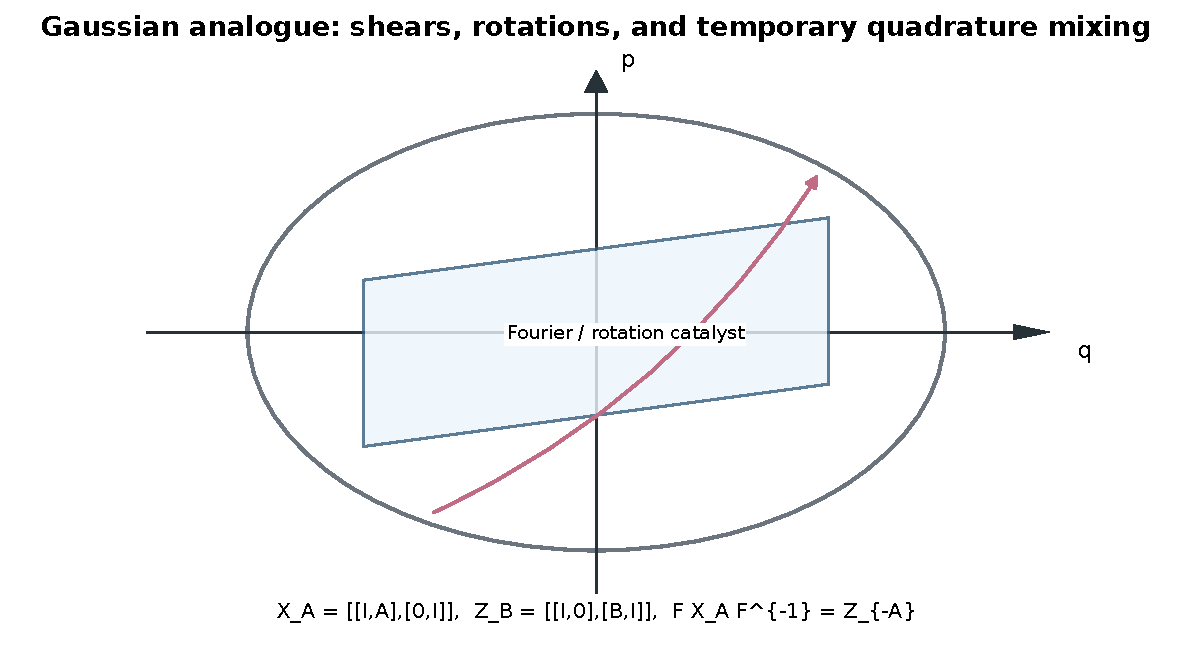
\includegraphics[width=.94\textwidth]{gaussian_shear_catalysis.pdf}
\caption{The row-transvection atom embedded as a Gaussian symplectic shear circuit.}
\label{fig:gaussian-shear}
\end{figure}

\section{Bosonic gate hierarchies}
Natural nested models include
\[
\text{triangular shears}
\subset
\text{all Gaussian unitaries}
\subset
\text{Gaussian plus a non-Gaussian primitive}
\subset
U(\mathcal H).
\]
Typical primitive resources are:
\begin{itemize}
\item SUM or controlled displacement gates,
\item beam splitters,
\item single-mode and two-mode squeezers,
\item Fourier transforms,
\item cubic phase gates,
\item photon counting or non-Gaussian state injection.
\end{itemize}
Each inclusion supports a different defect.  A target Gaussian transformation might be shortened by leaving a triangular decomposition but remaining Gaussian.  A more radical question asks whether temporary non-Gaussianity can shorten a final Gaussian target.

\section{Bloch--Messiah versus catalytic synthesis}
A bosonic Gaussian unitary admits a Bloch--Messiah decomposition
\[
S=K_1 D K_2,
\]
where $K_1,K_2$ are passive symplectic transformations and $D$ is a diagonal squeezing layer.  This normal form optimizes conceptual structure, not necessarily a weighted gate count on a specific architecture.

Catalytic synthesis asks whether a short excursion into a basis where many shear or squeezing obligations align can reduce total cost.  The opening and closing passive layers play the role of the catalyst.

\begin{skeletonbox}
A Gaussian catalytic theorem requires:
\begin{enumerate}
\item a declared primitive library and cost vector;
\item a target subgroup, such as triangular, number conserving, or local;
\item an explicit sandwich $KHK^{-1}$ returning to the target subgroup;
\item a lower bound based on symplectic rank, singular values, graph cuts, or mode support;
\item treatment of approximation error when continuous parameters are synthesized numerically.
\end{enumerate}
\end{skeletonbox}

\section{Fermionic Gaussian and matchgate circuits}
Let $c_j,c_j^\dagger$ be fermionic creation and annihilation operators.  Quadratic Hamiltonians generate Gaussian unitaries, and their action is determined by an orthogonal transformation on Majoranas.  Number-conserving Gaussian operations correspond to a unitary action on modes, while general Gaussian operations allow particle-hole mixing.

This yields the hierarchy
\[
\begin{gathered}
U(n)\text{ mode transformations}
\subset SO(2n)\text{ fermionic Gaussian transformations}\\
\subset \text{parity-preserving unitaries}.
\end{gathered}
\]
A temporary Bogoliubov transformation can violate number conservation while preserving parity.  The target may nevertheless return to the number-conserving subgroup.

\begin{definition}[Bogoliubov catalytic defect]
For a number-conserving Gaussian target $U$, compare the minimum cost using number-conserving primitives with the minimum cost using general Gaussian primitives, requiring the endpoint to conserve number exactly.
\end{definition}

\section{Matchgates and geometry}
Nearest-neighbor matchgate circuits \cite{Valiant2002,JozsaMiyake2008} have strong classical simulation properties.  Their geometry changes when SWAP, fermionic SWAP, long-range connectivity, or a single non-matchgate resource is added.  Candidate restricted/ambient pairs include:
\begin{enumerate}
\item nearest-neighbor matchgates versus all-to-all matchgates;
\item number-conserving matchgates versus general matchgates;
\item matchgates versus parity-preserving two-qubit gates;
\item Gaussian circuits versus Gaussian circuits with one reusable non-Gaussian ancilla.
\end{enumerate}

A compiler application is immediate: a temporary mode permutation or particle-hole rotation may allow a batch of otherwise expensive interactions to share one routing or basis-change layer.

\section{Covariance-matrix lower bounds}
For a Gaussian state, the covariance matrix $\Gamma$ transforms as
\[
\Gamma\longmapsto S\Gamma S^T
\]
in the bosonic case and
\[
\Gamma\longmapsto O\Gamma O^T
\]
in the fermionic case.  Possible restricted lower bounds include:
\begin{itemize}
\item rank change of off-diagonal covariance blocks,
\item symplectic singular-value obligations,
\item growth of mode support,
\item graph bandwidth and cut rank,
\item number of nontrivial canonical angles between invariant subspaces.
\end{itemize}
One elementary gate changes only a controlled portion of these data.  A useful invariant must also charge preparation of a carrier that makes progress on many cuts simultaneously.

\section{Temporary non-Gaussianity}
Suppose a non-Gaussian primitive $g$ is introduced and later removed:
\[
U=g h_m\cdots h_1 g^{-1},
\qquad U\in G_{\mathrm{Gauss}}.
\]
If $g h_i g^{-1}$ generates several useful Gaussian effects, the excursion may be catalytic.  However, many standard non-Gaussianity monotones vanish only on states rather than unitaries, and cancellation at the endpoint complicates direct lower bounds.

Candidate monotones and certificates include:
\begin{itemize}
\item degree in the Weyl characteristic function,
\item Wigner negativity generated during the path,
\item operator Schmidt rank across mode cuts,
\item polynomial degree of Heisenberg-evolved quadratures,
\item stabilizer rank for encoded finite-dimensional subspaces.
\end{itemize}

\section{Exact and numerical search}
Finite exact enumeration is available for binary symplectic or orthogonal quotients, but continuous Gaussian groups require a different strategy.
\begin{enumerate}
\item Fix a symbolic gate skeleton and solve polynomial equations for parameters.
\item Use interval arithmetic to certify nonexistence below a length.
\item Exploit canonical decompositions to quotient local or passive layers.
\item For discrete-angle Gaussian libraries, use exact algebraic-number arithmetic.
\item Store both an upper-bound circuit and a dual or algebraic certificate.
\end{enumerate}

\section{Architecture and routing}
On a line or grid, Gaussian and matchgate circuits may be dominated by routing.  Let $G_{\mathrm{conn}}$ be the hardware graph.  A mode permutation $\pi$ can be treated as a catalyst if it is opened, many interactions are executed in the reordered frame, and $\pi^{-1}$ restores the logical labeling.  The benefit is
\[
\text{routing saved across consumers}
-
2\,\text{cost}(\pi).
\]
This is the same amortization law as the linear snapshot family, now applied to mode geometry.

\begin{conjecturebox}
There exist number-conserving or nearest-neighbor Gaussian targets whose minimum weighted cost is reduced by a restored Bogoliubov, mode-permutation, or non-Gaussian excursion.  The first exact threshold depends on the primitive library and is not determined here.
\end{conjecturebox}

\section{Research deliverables}
A complete Gaussian extension should produce:
\begin{enumerate}
\item a finite or semialgebraic model with exact endpoint equality;
\item at least one nontrivial lower-bound invariant;
\item a minimal catalytic atom;
\item a weighted hardware interpretation;
\item a tensor or repeated-mode amplification theorem;
\item code using exact arithmetic or certified intervals.
\end{enumerate}

\chapter{Symmetry, ancillas, measurement, and architecture}\label{ch:symmetry-measurement}
\index{symmetry-preserving circuit}
\index{ancilla}
\index{measurement and feedforward}
\index{architecture constraint}
\index{resource theory}


\section{Beyond subgroup word metrics}
Some of the most important quantum resource enlargements are not inclusions of groups.  Measurement introduces branches, reset is irreversible, and ancillas enlarge the Hilbert space.  The appropriate abstraction is a nested pair of realization categories
\[
\mathcal C_{\mathrm{res}}
\subseteq
\mathcal C_{\mathrm{amb}},
\]
with a cost assigned to generating morphisms.

For a target channel $\Phi$ in the restricted category, define
\[
c_{\mathrm{res}}(\Phi)
=
\inf\{\cost(W):W\text{ realizes }\Phi\text{ in }\mathcal C_{\mathrm{res}}\}
\]
and similarly $c_{\mathrm{amb}}(\Phi)$.  The value $+\infty$ is allowed.  A finite positive difference is a metric defect; an infinite difference is an existence defect.

\section{Symmetry-preserving circuits}
Let $Q$ be a conserved charge and let
\[
H_Q=\{U:[U,Q]=0\}.
\]
Restricted circuits use gates commuting with $Q$.  Ambient circuits may temporarily leave $H_Q$ but must return to a charge-preserving endpoint.

Examples include:
\begin{itemize}
\item particle-number conservation,
\item parity conservation,
\item total spin or magnetization,
\item lattice gauge constraints,
\item stabilizer or CSS sector preservation,
\item block-diagonal representation sectors.
\end{itemize}

The Hilbert space decomposes as
\[
\mathcal H=\bigoplus_q\mathcal H_q.
\]
A restricted circuit is block diagonal.  An ambient catalyst may couple sectors, use the enlarged route, and decouple them at the endpoint.

\begin{skeletonbox}
A symmetry-breaking catalyst has three obligations:
\begin{enumerate}
\item quantify how far the path leaves the symmetry algebra;
\item prove exact return, not merely return on a chosen input state;
\item compare the cost with every symmetry-preserving realization of the full target operator.
\end{enumerate}
\end{skeletonbox}

\section{Sector-flow invariants}
Let $P_q$ be the projector onto sector $q$.  For an intermediate unitary $U_t$, define transfer blocks
\[
T_{q,r}(t)=P_q U_t P_r.
\]
A restricted path has $T_{q,r}=0$ for $q\ne r$.  Ambient paths may populate off-diagonal blocks.  Possible excursion measures include
\[
\sum_{q\ne r}\rank T_{q,r},
\qquad
\max_{q\ne r}\|T_{q,r}\|,
\qquad
\text{bandwidth in }|q-r|.
\]
These are analogues of strict-upper rank and bandwidth in the unitriangular theory.

\section{Clean and dirty ancillas}
A clean ancilla starts in a specified state, usually $\ket0$, and must be returned to that state.  A dirty ancilla starts in an unknown state and must be restored for every input.

Let $U$ act on the data register.  A clean-ancilla realization is a unitary $W$ satisfying
\[
W(\ket\psi\otimes\ket0)
=(U\ket\psi)\otimes\ket0
\quad\text{for every }\ket\psi.
\]
A dirty-ancilla realization requires
\[
W(\ket\psi\otimes\ket\phi)
=(U\ket\psi)\otimes\ket\phi
\quad\text{for every }\ket\psi,\ket\phi.
\]
The second condition is strictly stronger.

Ancillas define a family of defects
\[
\Delta_{a,\mathrm{clean}}(U),
\qquad
\Delta_{a,\mathrm{dirty}}(U),
\]
where $a$ is the number of ancillary qubits or modes.  Stable ancilla capacity asks whether a fixed number of reusable ancillas can yield an unbounded saving as the data size grows.

\section{Measurement and feedforward}
A measurement-assisted realization is described by an instrument with classical outcomes $m$, conditional channels $\Phi_m$, and feedforward operations.  Exact deterministic implementation of a unitary target requires every branch, after correction, to induce the same channel.

The cost vector may include
\[
(
T\text{-count},
\text{two-qubit count},
\text{measurement rounds},
\text{classical latency},
\text{ancilla qubits}
).
\]
A measurement can create an existence defect by realizing a channel unavailable unitarily under the same locality or depth constraints, or a metric defect by reducing one resource while increasing another.

\begin{definition}[Branch-catalytic realization]
A measurement-assisted circuit is branch catalytic when the intermediate classical or quantum branch information is absent from the final data channel and all declared work systems are reset or discarded according to the model.
\end{definition}

\section{Teleportation as a canonical ambient excursion}
Gate teleportation replaces direct implementation by:
\[
\text{prepare resource state}
\to
\text{entangle and measure}
\to
\text{classical correction}.
\]
The ambient category contains resources not present in the target channel: entanglement, measurement outcomes, and feedforward.  The endpoint can nevertheless be a deterministic unitary.

This is an archetypal realization defect, but careful accounting is mandatory.  A claimed saving must include resource-state preparation or explicitly treat the state as an external catalyst.

\section{Architecture-constrained gates}
Let $\Gamma=(V,E)$ be a hardware graph.  A restricted two-qubit gate may act only on edges of $E$.  The ambient model may permit a small number of nonlocal interactions, temporary logical relabelings, teleportation edges, or bus-mediated gates.

For a target $U$, define
\[
\ell_\Gamma(U)
=
\text{minimum hardware-respecting cost},
\]
and compare it with an enlarged graph $\Gamma'$.  A matched routing excursion has the form
\[
\pi
\;W\;
\pi^{-1},
\]
where $\pi$ is a logical permutation.  The excursion is profitable when many gates in $W$ become local in the permuted frame.

\begin{figure}[ht]
\centering
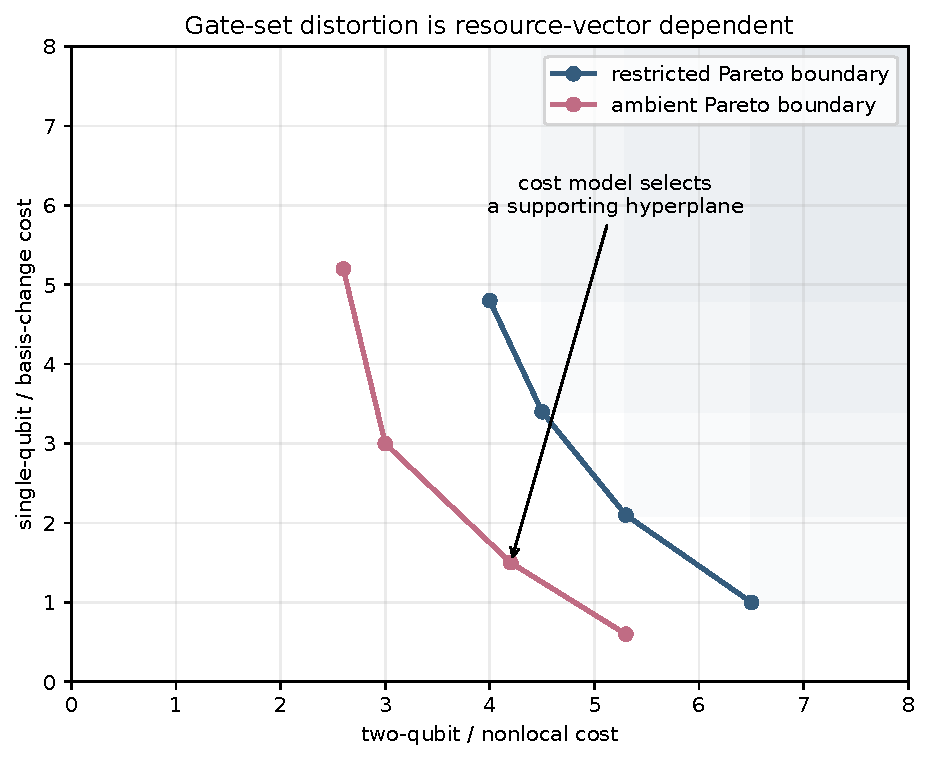
\includegraphics[width=.91\textwidth]{resource_pareto.pdf}
\caption{Gate-set defects generally live in a multi-resource Pareto geometry.}
\label{fig:resource-pareto}
\end{figure}

\section{Depth, count, and space-time volume}
Let $g_t$ be the set of gates scheduled in layer $t$.  Common scalar costs are
\[
\sum_t |g_t|,
\qquad
\#\{t:g_t\ne\varnothing\},
\qquad
\sum_t \#\{\text{active qubits in layer }t\}.
\]
A catalyst may reduce count but increase depth, or vice versa.  Space-time volume is often the more stable hardware quantity.

For stochastic error rates $p_g$, a first-order weighted cost is
\[
C_{\mathrm{err}}(W)=\sum_{g\in W}-\log(1-p_g).
\]
This additive approximation can be inserted directly into Dijkstra search.  It does not capture coherent or correlated errors, but it produces a declared and reproducible metric.

\section{Approximate synthesis}
For continuous gate sets, define
\[
\ell_{\mathrm{res},\varepsilon}(U)
=
\min\{\cost(W):\|W-U\|\le\varepsilon\}.
\]
There are two distinct border phenomena:
\begin{enumerate}
\item algebraic border length, where a target lies in the closure of a bounded exact word locus;
\item analytic approximation length, where an error tolerance is explicitly permitted.
\end{enumerate}
They should not be conflated.

A catalyst can improve the asymptotic Solovay--Kitaev or number-theoretic approximation constant even when exact synthesis is impossible in both models.

\section{Resource theories and monotones}
A quantum resource theory provides free states, free operations, and monotones.  Gate-set distortion adds a path-sensitive question: the endpoint may be free even though the path temporarily creates resource.

A state monotone $M(\rho)$ alone may fail because the catalyst acts at the channel level.  Useful channel-level quantities include:
\begin{itemize}
\item robustness or magic capacity,
\item entangling power,
\item operator Schmidt rank,
\item Choi-state resource measures,
\item symmetry asymmetry of the channel,
\item amortized resource generation.
\end{itemize}
A lower bound must relate the cumulative or peak resource to the declared gate cost and account for cancellation.

\section{A categorical amplification principle}
Suppose a monoidal category admits a tensor product and a cost satisfying
\[
c_{\mathrm{amb}}(f\otimes g)
\le
c_{\mathrm{amb}}(f)+c_{\mathrm{amb}}(g).
\]
If restricted cost is additive on a target family, then any one-copy defect amplifies linearly under independent tensor powers.  Superlinear amplification requires a normalization in which dimensions multiply, as in the matrix tensor rule of the core theory, or a joint-synthesis synergy across copies.

\section{Experimental standards}
Every architecture, measurement, or ancilla claim should state:
\begin{enumerate}
\item gate alphabet and native connectivity;
\item clean, dirty, catalytic, or consumable ancilla convention;
\item deterministic or postselected implementation;
\item exact or approximate endpoint condition;
\item total, weighted, depth, or Pareto cost;
\item whether resource-state preparation is included;
\item whether qubit relabeling is free;
\item certificate of restoration on all inputs.
\end{enumerate}
Without these declarations, two reported ``gate counts'' may refer to incomparable problems.

\begin{conjecturebox}
For several common symmetry and architecture restrictions, a constant-size restored excursion should yield an unbounded saving on structured target families.  The unitriangular construction proves this phenomenon for directed linear information flow; analogous theorems for charge sectors, measurement branches, and nonlocal routing remain open.
\end{conjecturebox}


\part{Packets, realization, and local-to-global structure}
\chapter{Packets, types, holonomy, and restricted realization}\label{ch:packets}
\index{spherical packet}
\index{type packet}
\index{holonomy packet}
\index{realization fiber}
\index{quantum Latin square}
\index{Langlands-style packet}


\section{Why coarse spectra are not enough}
A finite symmetry problem often comes with a natural commuting operator algebra.  Its joint spectrum is attractive because it is canonical, compact, and computationally cheap.  Yet the joint eigenvalues and their multiplicities can be identical across objects whose realization behavior is different.

This chapter develops the hierarchy
\begin{equation}\label{eq:packet-hierarchy}
\text{spherical packet}
\prec
\text{embedded type packet}
\prec
\text{holonomy packet}
\prec
\text{realization fiber}.
\end{equation}
The relation $\prec$ means ``retains strictly more potentially relevant information,'' not that every refinement is complete.

\begin{figure}[ht]
\centering
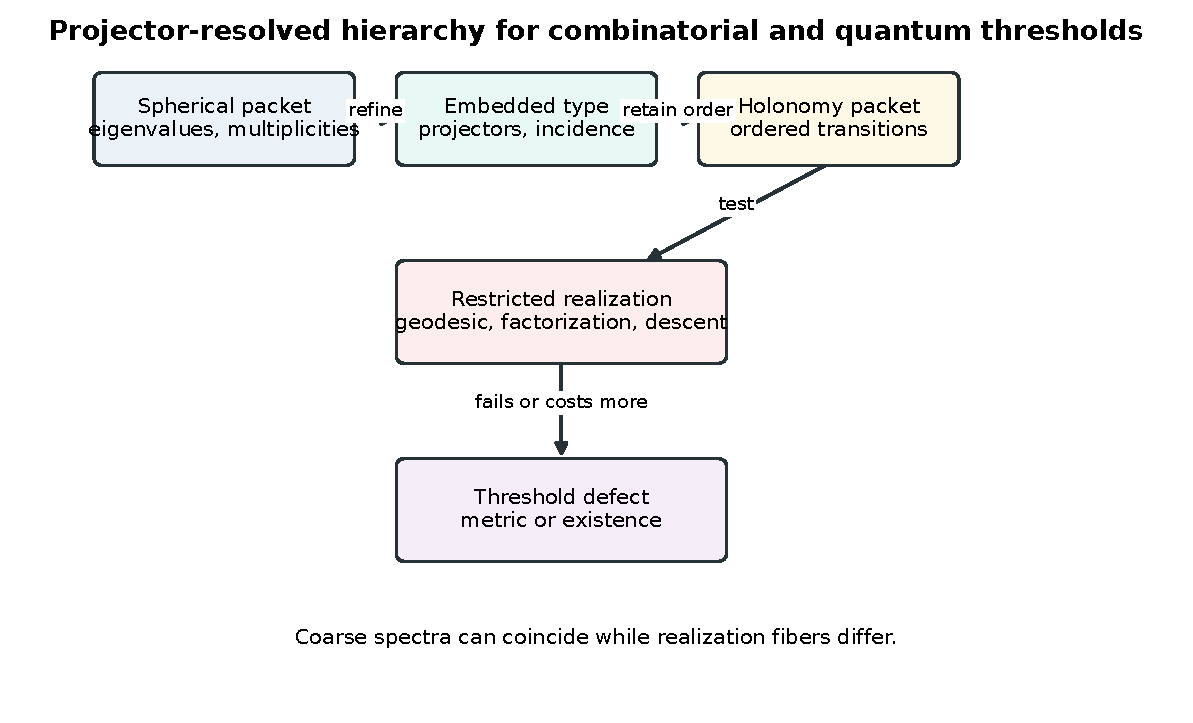
\includegraphics[width=.95\textwidth]{packet_hierarchy.pdf}
\caption{The packet hierarchy used to organize finite threshold systems.}
\label{fig:packet-realization-hierarchy}
\end{figure}

\section{Spherical packets}
Let $T_1,\ldots,T_m$ be commuting normal operators on a finite-dimensional Hilbert space.  Their unique coarsest joint spectral resolution is
\[
T_j=\sum_{\lambda}t_j(\lambda)B_\lambda,
\qquad
\sum_\lambda B_\lambda=I.
\]
The tuple
\[
\lambda=(t_1(\lambda),\ldots,t_m(\lambda))
\]
is the spherical label.  The abstract spectral packet records these labels and the ranks of $B_\lambda$.

Two different embedded systems can have the same abstract packet.  The actual matrices $B_\lambda$, endpoint coefficients, and transition operators may still differ.

\begin{principle}[Spherical collapse]
Passing from embedded operators to eigenvalues and multiplicities can erase exactly the incidence or transition data that controls restricted realization.
\end{principle}

\section{The Latin-square association algebra}
A Latin square $L$ of order $n$ has $n^2$ cells.  Let $R,C,S$ be adjacency matrices for equality of row, column, and symbol.  The algebra generated by $I,J,R,C,S$ is commutative and its abstract multiplication table depends only on $n$, not on the paratopy class of $L$.

Define
\[
Q_R=\frac{I+R}{n},
\qquad
Q_C=\frac{I+C}{n},
\qquad
Q_S=\frac{I+S}{n},
\qquad
B_0=\frac{J}{n^2}.
\]
Then the five joint projectors are
\[
B_0,
\quad Q_R-B_0,
\quad Q_C-B_0,
\quad Q_S-B_0,
\quad I-Q_R-Q_C-Q_S+2B_0.
\]
Their multiplicities are
\[
1,
\quad n-1,
\quad n-1,
\quad n-1,
\quad (n-1)(n-2).
\]
The Latin-square graph $R+C+S$ has universal spectrum
\[
3(n-1)^1,
\qquad
(n-3)^{3(n-1)},
\qquad
(-3)^{(n-1)(n-2)}.
\]
At $n=6$ this becomes
\[
15^1,\qquad3^{15},\qquad(-3)^{20}.
\]
Thus the graph spectrum cannot distinguish the twelve main classes of order six.

\begin{provedbox}
The displayed projector formulas depend only on the Latin-square axioms and the order.  They therefore prove that the abstract $R,C,S$ joint eigenvalue packets cannot distinguish squares of the same order.  This conclusion does not require an enumeration of the order-six main classes.
\end{provedbox}

\section{Transition fusion also collapses}
Let $\rho_i$ be the row permutations of a Latin square.  The symmetrized aggregate of all pair transitions satisfies
\begin{equation}\label{eq:transition-fusion}
\sum_{i<j}
\left(
P_{\rho_i\rho_j^{-1}}
+
P_{\rho_j\rho_i^{-1}}
\right)
=n(J-I).
\end{equation}
Hence first-order fusion destroys the class information as well.

The lesson is general: summing typed transitions can be as destructive as discarding the embedded projectors.  Order and labels matter.

\section{Embedded type data}
A type packet retains the actual projectors, support partitions, distinguished incidence sets, or local representation types.  Examples include:
\begin{itemize}
\item the row, column, and symbol partitions of a Latin square;
\item a projective-line closure system;
\item the flag stabilized by a circuit subgroup;
\item support patterns of unitary or quantum-Latin entries;
\item ramification or block data in a finite group action.
\end{itemize}

A projective-line closure procedure can supply additional type operators, such as adjacency operators of a line spread.  Whether a particular added operator separates two classes is a further question.  The present archive does not include the separate order-six projective computation, so it supplies no new finite certification of that comparison.

\section{Holonomy packets}
Let a family of local charts or rows be represented by permutations $\rho_i$.  Define normalized transitions
\[
h_{ij}=\rho_i\rho_j^{-1}
\]
and the transition group
\[
H_r(L)=\langle h_{ij}:i,j\rangle.
\]
A holonomy packet may include:
\begin{itemize}
\item the isomorphism type or order of $H_r(L)$,
\item the cycle-type inventory of the distinguished $h_{ij}$,
\item block systems and orbit partitions,
\item characters or matrix coefficients of words in the $h_{ij}$,
\item noncommutative moments
\[
\operatorname{tr}(h_{i_1j_1}\cdots h_{i_kj_k}),
\]
\item the corresponding packets for row, column, and symbol roles.
\end{itemize}

Isotopy conjugates these transition groups; paratopy permutes the three roles.  Therefore the unordered multiset of role signatures is a paratopy invariant.

\begin{skeletonbox}
For a specified collection of Latin squares, one can compute transition-group orders, pair-transition cycle inventories, and nontrivial block sizes, then test whether the resulting role signatures separate the collection.  The separate order-six input tables and verifier are not included in this archive, so pairwise separation of all twelve main classes is an open verification obligation here.
\end{skeletonbox}
Even a complete discrete classification would not prove orthonormal representability.  Noncommutative transition data are candidate refinements of the information lost under spherical fusion.

\section{Imprimitivity as hidden decomposition}
A transitive permutation group is imprimitive when it preserves a nontrivial block system.  In combinatorial designs, imprimitivity often signals a subsquare, product, congruence, or module decomposition.

For a Latin square of order $2m$, normalize one row to the identity permutation on the symbols.  An $m\times m$ Latin subsquare determines a partition of the symbols into its $m$ symbols and their complement.  Rows meeting the subsquare preserve the two corresponding column blocks, and the remaining rows exchange them.  Thus normalized row transitions preserve this two-block system.  Conversely, if all normalized row transitions preserve a partition into two blocks of size $m$, exactly $m$ rows send a fixed column block into a fixed symbol block, producing an $m\times m$ Latin subsquare.  This is a structural criterion.  Counting the order-six classes with this property requires separate input representatives.

\begin{principle}[Clifford-type decomposition]
Combinatorial substructure can be detected as imprimitivity of a transition packet.  The spherical packet sees aggregate multiplicities; the holonomy packet sees how those multiplicities are assembled into blocks.
\end{principle}

\section{Realization fibers}
Let $P$ denote packet data and let
\[
\operatorname{Real}_{\mathrm{res}}(P)
\]
be the space of restricted realizations compatible with $P$.  The packet may completely classify the discrete object while the realization fiber remains empty, positive dimensional, disconnected, or singular.

Examples of realization conditions include:
\begin{itemize}
\item a flag-preserving geodesic with a declared length;
\item a product-state orthonormal representation;
\item a positive semidefinite Gram matrix with a zero pattern;
\item a tensor factorization;
\item a global descent object compatible with local packets;
\item a circuit satisfying ancilla restoration on every input.
\end{itemize}

Thus classification and realization are distinct layers.

\section{Quantum Latin squares as an existence defect}
A quantum Latin square is an array \cite{MustoVicary2016} of vectors whose rows and columns are orthonormal bases.  Ball and Simoens prove that a pair of non-entangled mutually orthogonal quantum Latin squares of order six does not exist, while earlier work provides entangled order-six solutions and hence AME$(4,6)$ states \cite{BallSimoens2026,RatherEtAl2022,RatherEtAl2023}.

This is naturally expressed as
\[
\operatorname{Real}_{\mathrm{product}}(P_6)=\varnothing,
\qquad
\operatorname{Real}_{\mathrm{entangled}}(P_6)\ne\varnothing.
\]
It is an existence defect, not a gate-count defect.

\begin{figure}[ht]
\centering
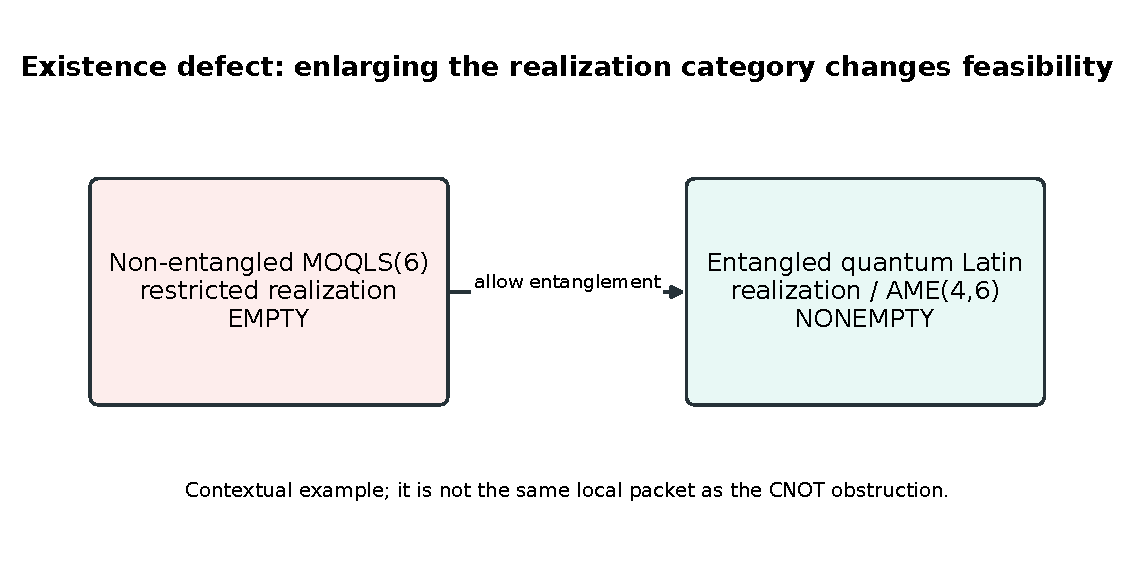
\includegraphics[width=.92\textwidth]{quantum_latin_realization_gap.pdf}
\caption{The order-six quantum-Latin distinction is a restricted-versus-ambient realization gap.}
\label{fig:quantum-latin-gap}
\end{figure}

The source proof uses support patterns, a reduction to one classical square, orthonormal representations of complements of Latin-square graphs, projective-line closure, finite case analysis over twelve main classes, and a continuous argument for the two remaining subsquare cases.  No theorem in the unitriangular or Clifford chapters is inferred from this result.

\section{First-arrival packets}
For a finite generator set $S$, the endpoint Green kernel
\[
\mathcal G_{S,g}(z)
=
\langle\delta_g,(I-zA_S)^{-1}\delta_e\rangle
\]
contains more information than the spectrum of $A_S$.  Its first nonzero degree is the distance to $g$.

If
\[
A_S=\sum_\lambda \lambda B_\lambda,
\]
then
\[
\mathcal G_{S,g}(z)
=
\sum_\lambda
\frac{\langle\delta_g,B_\lambda\delta_e\rangle}{1-\lambda z}.
\]
The endpoint matrix coefficients of the embedded projectors determine cancellation between spectral components.  This is the metric analogue of retaining a type rather than only an unramified eigencharacter.

\section{Typed Green kernels}
Let $H\le G$ and let $\mu_k(h)$ count ambient words of length $k$ with holonomy $h\in H$.  For an irreducible representation $\tau$ of $H$, define
\[
\widehat\mu_k(\tau)
=
\sum_{h\in H}\mu_k(h)\tau(h)
\]
and
\[
\widehat{\mathcal G}_\tau(z)
=
\sum_{k\ge0}\widehat\mu_k(\tau)z^k.
\]
Fourier inversion recovers every $\mu_k(h)$.  The trivial representation records only total return to the subgroup; nontrivial types resolve the holonomy.

\begin{provedbox}
For finite $H$, the full family of typed Green kernels over $\widehat H$ determines every endpoint Green series and therefore every ambient word distance from the identity to an element of $H$.
\end{provedbox}

\section{Operational Langlands analogy}
The hierarchy resembles the local organization of representation theory:
\[
\text{spherical character}
\to
\text{type}
\to
\text{ramification or monodromy}
\to
\text{realization and descent}.
\]
The analogy is useful because it prevents coarse spectral data from being mistaken for a complete correspondence.  It does not imply that global Langlands reciprocity predicts either the circuit threshold or the quantum-Latin result.

\begin{boundarybox}
The word ``Langlands'' in this monograph refers to an operational packet architecture: commuting local spectra, type refinement, noncommutative holonomy, tensor assembly, and descent obligations.  No general automorphic or Galois correspondence is claimed or used.
\end{boundarybox}

\section{A general finite threshold system}
A packet-resolved threshold system consists of:
\begin{enumerate}
\item a finite group, groupoid, or association scheme;
\item a commutative spherical algebra with exact projectors;
\item embedded incidence or type data;
\item a transition group or monodromy representation;
\item restricted and ambient realization categories;
\item a metric, multiplicity, or descent obstruction.
\end{enumerate}

The first threshold may then be defined as
\[
\tau=
\min\{n:\exists P\text{ with }c_{\mathrm{res}}(P)>c_{\mathrm{amb}}(P)\}.
\]
The cost can be finite or infinite.

\section{Open problems}
\begin{question}
For which finite association schemes does the full embedded Bose--Mesner algebra determine the restricted realization fiber?
\end{question}
\begin{question}
What bounded degree of noncommutative transition moments separates all Latin squares of a fixed order?
\end{question}
\begin{question}
Can typed Green kernels yield new lower bounds without enumerating the full ambient group?
\end{question}
\begin{question}
When does imprimitivity of a transition packet characterize a tensor or subsquare decomposition in quantum combinatorial designs?
\end{question}


\part{Computational atlas and theorem templates}
\chapter{The exact computational atlas}\label{ch:atlas}
\index{breadth-first search}
\index{zero-one BFS}
\index{Dijkstra algorithm}
\index{certificate}
\index{reproducibility}


\section{Purpose and design}
The accompanying code is an audit-oriented finite mathematics package rather than a production compiler.  Its goals are:
\begin{enumerate}
\item exact state representations with no floating-point ambiguity;
\item complete finite search where the state space is tractable;
\item explicit witnesses and reconstructible paths;
\item small, dependency-free core algorithms;
\item frozen JSON results and regression tests;
\item separation between proved, computed, and proposed claims.
\end{enumerate}

The package is named \texttt{catalytic\_gate\_atlas}.  Binary matrices are tuples of integer row bitmasks, and reversible Boolean maps are exact permutations of basis-state indices.

\begin{figure}[ht]
\centering
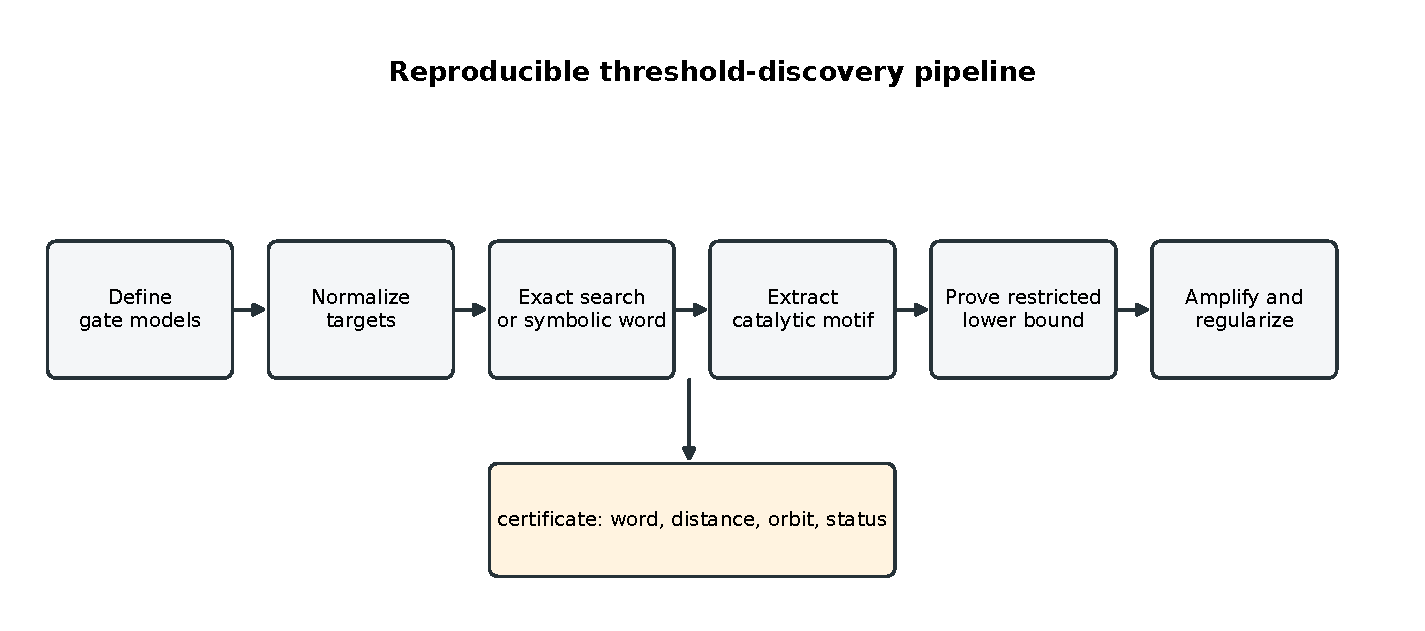
\includegraphics[width=.96\textwidth]{computational_pipeline.pdf}
\caption{The finite certificate pipeline used throughout the computational atlas.}
\label{fig:computational-pipeline}
\end{figure}

\section{State models}
\subsection{Binary matrices}
An $m\times m$ matrix over $\F_2$ is stored as
\[
(r_0,\ldots,r_{m-1}),
\]
where bit $j$ of $r_i$ is the $(i,j)$ entry.  Matrix multiplication is exact XOR accumulation.

\subsection{Symplectic Clifford states}
An $n$-qubit Clifford modulo global phase and Pauli translation is represented by its action on Pauli exponent vectors
\[
(x\mid z)\in\F_2^{2n}.
\]
The state space is $\Sp(2n,2)$.  The restricted parabolic group is generated by $S$, CZ, and CNOT; the ambient group additionally permits $H$.

\subsection{Classical reversible states}
A reversible map on $n$ bits is stored as a permutation of $\{0,\ldots,2^n-1\}$.  Composition is exact.  The affine subgroup is generated by $X$ and CNOT, and the ambient three-bit group adds Toffoli.

\section{Shortest-path engines}
The package implements:
\begin{itemize}
\item breadth-first search for unit costs;
\item $0$--$1$ breadth-first search when gates are free or unit cost;
\item Dijkstra search for general nonnegative integer weights;
\item parent maps for witness reconstruction;
\item defect distributions on a restricted target set.
\end{itemize}

\begin{algorithm}[Breadth-first defect census]
Given restricted generators $S_R$, ambient generators $S_A$, and identity $e$:
\begin{enumerate}
\item compute $d_R$ on $\langle S_R\rangle$;
\item compute $d_A$ on $\langle S_A\rangle$;
\item for every restricted state $x$, compare $d_R(x)$ and $d_A(x)$;
\item record the pair $(d_R(x),d_A(x))$ and reconstruct witnesses for strict inequalities.
\end{enumerate}
\end{algorithm}

For a finite group this is complete because every vertex reachable from the identity is visited exactly once at its minimum distance.

\section{Zero-cost gates}
When local Clifford gates are free and entangling gates cost one, ordinary BFS is invalid.  The package uses a deque-based $0$--$1$ BFS.  A zero-cost edge is pushed to the front and a unit-cost edge to the back.  The resulting labels are exact shortest entangling costs.

A common error is to quotient by free gates without proving that the quotient preserves the target subset and all left/right actions.  The atlas avoids this issue by running $0$--$1$ BFS directly on the finite group for the reported small cases.

\section{The optimized Clifford verifier}
The three-qubit symplectic group has
\[
|\Sp(6,2)|=1{,}451{,}520
\]
states.  A compact C++ implementation enumerates the full group and the parabolic subgroup exactly.  It supports:
\begin{itemize}
\item total primitive count;
\item total count with unit-cost SWAP;
\item entangling count with $H$ and $S$ free;
\item exact distance distributions and JSON output.
\end{itemize}
The C++ program and the independent Python implementation use the same gate matrices but different traversal code.  Witness reconstruction is supplied by the Python implementation, not by the C++ census executable.

\section{Computed Clifford census}
\begin{longtable}{@{}ccccccc@{}}
\toprule
$n$ & Metric & SWAP & $|P_n|$ & $|\Sp(2n,2)|$ & Defects & Max defect\\
\midrule
1 & total & no & 2 & 6 & 0 & 0\\
1 & entangling & no & 2 & 6 & 0 & 0\\
2 & total & no & 48 & 720 & 0 & 0\\
2 & entangling & no & 48 & 720 & 4 & 1\\
3 & total & no & 10,752 & 1,451,520 & 24 & 1\\
3 & total & yes & 10,752 & 1,451,520 & 0 & 0\\
3 & entangling & no & 10,752 & 1,451,520 & 1,624 & 2\\
\bottomrule
\end{longtable}

The detailed defect distributions are:
\[
\begin{array}{c|l}
\text{model}&\text{restricted}\to\text{ambient pairs}\\
\hline
n=2\text{ entangling}&3\to2:4\\
n=3\text{ total}&7\to6:6,\quad8\to7:18\\
n=3\text{ entangling}&3\to2:24,\ 4\to3:432,\ 5\to4:1056,\ 6\to4:48,\ 6\to5:64.
\end{array}
\]

\begin{computedbox}
Every entry in the table is a complete finite enumeration in the declared binary symplectic model.  Phases and Pauli translations are not part of the state space.  These are exact results for that quotient model, not full hardware Clifford optimizations.
\end{computedbox}

\section{Computed affine-versus-Toffoli census}
For three bits:
\[
|\operatorname{AGL}(3,2)|=1344,
\qquad
|S_8|=40320.
\]
The complete census finds no affine target with a strict defect under total primitive count or under entangling count with NOT free.

\begin{longtable}{@{}ccccc@{}}
\toprule
Metric & Restricted size & Ambient size & Restricted diameter & Defects\\
\midrule
Total & 1,344 & 40,320 & 7 & 0\\
Entangling & 1,344 & 40,320 & 6 & 0\\
\bottomrule
\end{longtable}

\section{Linear symbolic checks}
The Python module verifies that the displayed six-row ambient and restricted words produce the same canonical target modulo
\[
2,3,5,8.
\]
The lower bounds and ring universality are proved in the core chapter; these modular checks are regression tests rather than the logical basis of the theorem.

\section{Witness format}
A witness record contains:
\begin{itemize}
\item the target matrix or permutation;
\item restricted and ambient costs;
\item a named restricted gate path;
\item a named ambient gate path;
\item the metric and gate alphabet;
\item the state-model convention.
\end{itemize}
For example, the two-qubit entangling Clifford witness has restricted path
\[
\CX_{0\to1},\ S_1,\ \CX_{1\to0},\ \CX_{0\to1}
\]
and ambient path
\[
H_1,\ \CX_{1\to0},\ \CX_{0\to1},\ H_0,\ S_1,\ S_0.
\]
Only two gates in the ambient path are charged by the entangling metric.

\section{Certificates beyond full enumeration}
For larger systems, the following certificate styles are supported in principle.
\begin{enumerate}
\item \textbf{Meet in the middle.}  Store forward and backward balls whose radii sum to the candidate length.
\item \textbf{SAT/SMT.}  Encode gate choices and endpoint equations; use an UNSAT certificate below the claimed optimum.
\item \textbf{Integer programming.}  Useful when a fixed gate skeleton leaves discrete routing choices.
\item \textbf{Algebraic elimination.}  Eliminate continuous gate parameters from bounded-length word equations.
\item \textbf{Dual potentials.}  Exhibit a one-Lipschitz potential attaining the claimed lower bound.
\item \textbf{Quotient search.}  Search cosets only after proving that the quotient is compatible with the cost and target class.
\end{enumerate}

\section{Multiobjective search}
Let each gate have a vector cost in $\N^r$.  At each state, retain only nondominated labels.  The algorithm terminates for finite state spaces with a bounded search region, but the frontier can grow exponentially.

A practical exact strategy is to scalarize with several positive weight vectors, use the resulting optima to identify candidate Pareto points, and then certify each candidate by constrained search.

\section{Reproducibility commands}
From the \texttt{code} directory:
\begin{lstlisting}[style=pythonstyle,caption={Python atlas commands.}]
python -m pip install -e . --no-build-isolation
python scripts/run_atlas.py --output ../results/atlas_small.json
python -m pytest tests
\end{lstlisting}
The optimized three-qubit verifier can be compiled by
\begin{lstlisting}[style=cppstyle,caption={C++ Clifford verifier.}]
g++ -O3 -std=c++20 scripts/clifford_census.cpp -o scripts/clifford_census
./scripts/clifford_census --n 3 --metric total --output ../results/clifford_n3_total.json
./scripts/clifford_census --n 3 --metric entangling --output ../results/clifford_n3_entangling.json
\end{lstlisting}

\section{Validation policy}
The release uses four layers of validation.
\begin{enumerate}
\item Unit tests for matrix, permutation, and path primitives.
\item Cross-checks of group sizes against known finite formulas.
\item Independent Python and C++ computations for selected Clifford cases.
\item Frozen JSON outputs and SHA-256 manifests in the release archive.
\end{enumerate}

\section{Scaling limits}
Full group enumeration grows rapidly:
\[
|\Sp(2n,2)|
=2^{n^2}\prod_{j=1}^n(4^j-1).
\]
The four-qubit symplectic group is far beyond direct Python BFS.  Future work should exploit:
\begin{itemize}
\item double-coset normal forms,
\item Bruhat or parabolic decompositions,
\item admissible heuristics for A* search,
\item SAT encodings,
\item orbit reduction,
\item tensor-network representations,
\item distributed meet in the middle.
\end{itemize}

\section{What the atlas does not prove}
A finite census establishes only the declared finite model.  It does not prove:
\begin{itemize}
\item an asymptotic theorem without a separate proof,
\item a hardware advantage under a different cost,
\item robustness to approximation,
\item equivalence after adding ancillas,
\item a result for global phases or Pauli translations if they were quotiented out.
\end{itemize}
The status metadata in every result file is intended to make these boundaries machine readable.

\chapter{Reusable theorem templates}\label{ch:templates}
\index{theorem template}
\index{lower bound}
\index{dimension per gate}
\index{tensor amplification}


\section{Purpose}
This chapter collects proof architectures that recur across gate logics.  Each template separates the easy upper-bound identity from the difficult lower-bound obligation.  The templates are not claims that every gate hierarchy satisfies the hypotheses.

\section{Template I: catalytic conjugation}
Let $H\le G$ have restricted and ambient costs with $\ellAmb(g^{-1})=\ellAmb(g)$.  Choose $g\in G$ and $h_1,\ldots,h_m\in H$ such that
\[
U=g h_m\cdots h_1 g^{-1}\in H.
\]
Then
\[
\ellAmb(U)
\le
2\ellAmb(g)+\sum_i\ellAmb(h_i).
\]

\begin{theorem}[Catalytic comparison template]
Assume a restricted lower bound of the form
\[
\ellRes(U)
\ge
\sum_i r_i-\beta,
\]
where $r_i$ is the restricted cost of the $i$th transported obligation and $\beta$ is the maximum certified sharing.  Then
\[
\Delta(U)
\ge
\sum_i r_i-\beta
-
2\ellAmb(g)-\sum_i\ellAmb(h_i).
\]
\end{theorem}

The proof is immediate.  The research content lies in bounding $\beta$.

\section{Template II: amortized consumers}
Suppose a catalyst costs $c_{\mathrm{open}}+c_{\mathrm{close}}$ and each of $m$ consumers saves at least $s_i$ restricted cost.  Then
\[
\Delta(U)
\ge
\sum_{i=1}^m s_i
-c_{\mathrm{open}}-c_{\mathrm{close}}-r,
\]
where $r$ is repair or interference cost.  A threshold occurs when the right side first becomes positive.

This template explains the three-cross rule in the linear atom and guides searches in phase, Gaussian, and routing models.

\section{Template III: first-arrival Green valuation}
Let $S$ be a finite symmetric generating set and
\[
A_S=\sum_{s\in S}\rho(s).
\]
Then
\[
\mathcal G_{S,g}(z)
=\sum_{k\ge0}\langle\delta_g,A_S^k\delta_e\rangle z^k.
\]

\begin{theorem}[First-arrival template]
If word multiplicities are nonnegative, then
\[
d_S(e,g)=\ord_{z=0}\mathcal G_{S,g}(z).
\]
For restricted and ambient sets,
\[
\Delta(g)=\ord_0\mathcal G_{S_R,g}-\ord_0\mathcal G_{S_A,g}.
\]
\end{theorem}

This template provides an exact spectral restatement.  To turn it into a lower bound without enumeration, one needs control of the endpoint projector coefficients.

\section{Template IV: one-Lipschitz potentials}
Let $F$ be a function on circuit states satisfying
\[
F(I)=0,
\qquad
|F(gs)-F(g)|\le c(s)
\]
for every allowed restricted gate $s$.  Then
\[
\ellRes(U)\ge F(U).
\]

Potential design steps:
\begin{enumerate}
\item choose a decomposition into cuts, packets, or degree layers;
\item prove a gate changes the total charge by at most its cost;
\item ensure cancellations cannot create free progress on many layers;
\item evaluate the target exactly.
\end{enumerate}
Static sums of ranks are often too coarse in ambient models; time-expanded or target-relative potentials may be required.

\section{Template V: dimension per gate}
Let $X$ be an algebraic family of elementary gates whose irreducible components have dimension at most $r$.  Let $V$ be an irreducible target variety of dimension $N$.

\begin{theorem}[Dimension-per-gate template]
The closure of the locus reachable in $L$ gates has dimension at most $rL$.  If $rL<N$, a generic point of $V$ is not reachable in $L$ gates.
\end{theorem}

If every target in $V$ has a restricted construction of length at most $N/r$, then generic restricted and ambient lengths coincide at that value, provided the same parameter bound applies to the ambient alphabet.

\section{Template VI: defect codimension}
Assume every target has restricted cost at most $M$.  A defect of size at least $d$ implies ambient cost at most $M-d$.  If the $(M-d)$-gate ambient locus has dimension at most $N-d$, then
\[
\codim\overline{\mathcal D_{\ge d}}\ge d.
\]
This is the general mechanism behind algebraic rarity.

\section{Template VII: finite-field sparsity}
Suppose there are at most $B$ gate directions and at most $q^r$ parameter choices per gate over $\F_q$.  Then the number of words of length at most $L$ is at most
\[
\sum_{j=0}^L(Bq^r)^j.
\]
If the target family has $q^N$ points and defect $d$ forces $L\le (N-d)/r$, this yields a density bound of order $q^{-d}$ up to a fixed combinatorial factor.

The estimate counts words, not distinct endpoints, and is therefore an upper bound without injectivity assumptions.

\section{Template VIII: block retraction}
Let a large restricted group contain a smaller one through a homomorphic embedding $\iota$, and suppose a homomorphic retraction $\pi$ satisfies $\pi\iota=\operatorname{id}$.  Require that every large restricted generator maps to a small restricted word of no greater cost.  Then
\[
\ell_{\mathrm{large,res}}(\iota U)
\ge
\ell_{\mathrm{small,res}}(U).
\]
If the ambient embedding preserves gate cost,
\[
\Delta_{\mathrm{large}}(\iota U)
\ge
\Delta_{\mathrm{small}}(U).
\]
This transfers a catalytic atom to architectures containing it as a retract.

\section{Template IX: exact block coupling}
For block-lower matrices
\[
M=
\begin{pmatrix}
A&0\\
XA&D
\end{pmatrix},
\]
projection to diagonal blocks forces the costs of $A$ and $D$, while rank of the cross block forces at least $\rank X$ cross transmissions.  If $X$ is a partial monomial matrix, the lower bound is attained by direct construction.

The same logic extends to trees of blocks whenever every coupling layer has an exact rank certificate and the projections are homomorphisms.

\section{Template X: tensor Leibniz rule}
Suppose a restricted complexity is tree tight and satisfies
\[
\ellRes(A\otimes B)
=n\ellRes(A)+m\ellRes(B)
\]
for $A$ of size $m$ and $B$ of size $n$.  If ambient complexity satisfies the corresponding upper bound, then
\[
\Delta(A\otimes B)
\ge
n\Delta(A)+m\Delta(B).
\]
For tensor powers,
\[
\Delta(A^{\otimes r})
\ge
r m^{r-1}\Delta(A).
\]
This is the standard route from a finite atom to an $N\log N$ defect.

\section{Template XI: stable capacity}
If
\[
a_{r+s}\le m^s a_r+m^r a_s,
\]
then
\[
b_r=\frac{a_r}{m^{r-1}}
\]
is subadditive and
\[
\lim_{r\to\infty}\frac{a_r}{r m^{r-1}}
\]
exists by Fekete's lemma.  This defines a regularized ambient cost and exposes possible tensor activation.

\section{Template XII: vector costs}
Let gates carry costs in $\R_+^k$.  A lower bound may be a vector inequality
\[
F(U)\preceq\sum_{g\in W}c(g)
\]
or a family of scalar inequalities indexed by dual weights $w\in\R_+^k$:
\[
w\cdot F(U)\le w\cdot c(W).
\]
A complete Pareto proof may require enough supporting weights to separate the restricted and ambient convex lower hulls.

\section{Template XIII: ancilla restoration}
Let $W$ act on data $D$ and ancilla $A$.  To certify a dirty catalyst, prove the operator identity
\[
W=U_D\otimes I_A
\]
on the full joint space, not only on one ancilla input.  For a clean catalyst, prove
\[
W(\ket\psi\otimes\ket0)
=(U\ket\psi)\otimes\ket0
\]
for all $\ket\psi$.  The distinction changes both the target equations and lower bounds.

\section{Template XIV: symmetry-sector escape}
Given projectors $P_q$, define off-sector transfer blocks
\[
T_{qr}=P_qUP_r.
\]
A restricted gate preserves all diagonal sectors.  An ambient gate changes a controlled collection of blocks.  A candidate potential is a weighted sum of ranks or norms of obligations relative to the final target.  The proof must charge both creation and useful consumption of off-sector coherence.

\section{Template XV: exhaustive threshold classification}
A finite first-threshold theorem should contain:
\begin{enumerate}
\item no defects below size $n_0$;
\item at least one defect at $n_0$;
\item exact classification of every defect at $n_0$ modulo declared equivalence;
\item analytic generation of the exceptional motifs;
\item equality between the analytic set and computational census;
\item witness and completeness certificates.
\end{enumerate}
This is the standard achieved by the six-wire linear core and is the target standard for future gate logics.

\section{A proof-obligation ledger}
Before promoting a catalytic identity to a theorem, record:
\begin{longtable}{@{}p{.29\textwidth}p{.62\textwidth}@{}}
\toprule
Obligation & Required evidence\\
\midrule
Endpoint membership & Symbolic proof that the target lies in the restricted class.\\
Ambient upper bound & Explicit circuit evaluated exactly.\\
Restricted lower bound & Potential, rank, algebraic, search, or certificate argument.\\
Restoration & Identity on all data and work inputs under the chosen convention.\\
Cost compatibility & Same gate alphabet, weights, and free operations in both metrics.\\
Minimal threshold & Exhaustive or symbolic exclusion of smaller instances.\\
Equivalence classification & Orbit or normal-form analysis of all minimal defects.\\
Amplification & Proof that the lower bound and upper construction compose.\\
Reproducibility & Source, frozen outputs, and deterministic commands.\\
\bottomrule
\end{longtable}

\chapter{Research program and paper architecture}\label{ch:program}
\index{open problem}
\index{research program}


\section{The central research problem}
For a nested pair of gate models, determine the distortion function
\[
D_n=
\sup_{U\in\mathcal T_n}
\bigl(c_{\mathrm{res}}(U)-c_{\mathrm{amb}}(U)\bigr),
\]
where $\mathcal T_n$ is the target class.  The basic questions are:
\begin{enumerate}
\item Does any defect exist?
\item What is the first size threshold?
\item What is the minimal catalytic motif?
\item Is the effect generic, sparse, or confined to special strata?
\item How does it scale under direct sum, recursion, and tensor products?
\item Which resource vector reveals the first defect?
\item Can the effect survive realistic architecture and fault-tolerant costs?
\end{enumerate}

\section{Established base camp}
The unitriangular theory provides a complete first example:
\begin{itemize}
\item a universal six-row atom over nonzero commutative rings;
\item exact binary and ternary first-threshold evidence;
\item exact classification of twenty binary minimal defects;
\item connected families with two reverse gates and linear saving;
\item microscopic rank-one, bandwidth-one escape;
\item generic rigidity and defect codimension;
\item recursive and tensor amplification to $\Omega(n\log n)$.
\end{itemize}
The small Clifford atlas adds a second gate logic with genuine exact defects and shows that changing the primitive library by adding SWAP can remove them.

\section{Program A: complete the Clifford threshold theory}
The highest-priority quantum project is a paper on parabolic-versus-ambient Clifford synthesis.

\subsection{Immediate tasks}
\begin{enumerate}
\item Extend the analytic four-target free-phase orbit certificate to other cost-preserving Clifford equivalences and larger widths.
\item Classify the twenty-four three-qubit total-count defects under parabolic conjugation and qubit permutations.
\item Derive analytic normal forms for the witness circuits.
\item Prove lower bounds independent of full group enumeration.
\item Test depth, weighted, and architecture-aware metrics.
\item Determine whether a finite defective atom tensor-amplifies.
\end{enumerate}

\subsection{Longer-term questions}
\begin{conjecture}
The parabolic subgroup of $\Sp(2n,2)$ has unbounded additive distortion in the full symplectic group for at least one natural Clifford cost model.
\end{conjecture}
\begin{question}
Does the maximum total-count defect grow as $n$, $n\log n$, or faster?
\end{question}
\begin{question}
Is the disappearance of three-qubit defects after adding unit-cost SWAP a small-width accident or a structural geodesic-convexity phenomenon?
\end{question}

\section{Program B: temporary nonlinearity}
The three-bit affine-versus-Toffoli census is rigid.  The next target is a complete four-bit normal-form search without enumerating $16!$ permutations.

\subsection{Algorithmic plan}
\begin{enumerate}
\item Compute exact affine distances for all $|\operatorname{AGL}(4,2)|=322{,}560$ targets.
\item Enumerate Toffoli sandwiches modulo affine left and right actions.
\item Use ANF equations to retain only affine endpoints.
\item Compare total, Toffoli, CNOT, and fault-tolerant costs.
\item Produce SAT certificates below every claimed optimum.
\end{enumerate}

\begin{question}
What is the first bit width at which a restored nonlinear excursion shortens an affine target?
\end{question}
\begin{question}
Can temporary degree two yield a family with unbounded saving while the endpoint degree remains one?
\end{question}

\section{Program C: phase-polynomial catalysts}
The phase setting is likely to produce a defect first in a resource other than total primitive count.

Priority metrics:
\[
T\text{-depth},
\quad
\text{CNOT count at fixed }T\text{-count},
\quad
\text{two-qubit depth},
\quad
\text{architecture-weighted cost}.
\]
A first paper should choose one metric and avoid a diffuse comparison across all resources.

\begin{question}
Can a restored Hadamard or Clifford frame reduce $T$-depth of a diagonal target without additional ancillas?
\end{question}
\begin{question}
Does tensor activation occur for phase-polynomial $T$-count?
\end{question}

\section{Program D: Gaussian and matchgate systems}
Two concrete first searches are recommended.
\begin{enumerate}
\item Number-conserving versus general fermionic Gaussian synthesis on a small number of modes.
\item Nearest-neighbor versus all-to-all matchgate circuits with weighted fermionic SWAP cost.
\end{enumerate}
Both admit exact orthogonal-matrix representations and have clear architecture relevance.

\section{Program E: symmetry and measurement}
This program should begin with a narrowly declared resource theory, such as:
\begin{itemize}
\item excitation-preserving two-qubit gates versus arbitrary two-qubit gates;
\item unitary Clifford+$T$ versus measurement-assisted Clifford+$T$;
\item clean versus dirty ancillas for a fixed arithmetic family;
\item local architecture versus one reusable nonlocal bus gate.
\end{itemize}
The first objective is not maximal generality but one theorem with exact restoration and cost accounting.

\section{Program F: root-system catalysis}
For a split reductive group with allowed roots $\Psi\subset\Phi$, classify configurations in which a forbidden root acts as a reusable catalyst through Chevalley commutator relations.

Suggested sequence:
\[
A_2\to B_2=C_2\to G_2\to A_r.
\]
Low-rank nonsimply laced systems are attractive because longer root strings may create more than one useful effect per consumer.

\begin{question}
Is there a root-system analogue of the three-cross, one-phase threshold?
\end{question}
\begin{question}
Can a $G_2$ root string produce a multiplicative distortion exceeding the clean type-$A$ value $3/2$?
\end{question}

\section{Program G: algebraic defect loci}
For each finite-dimensional gate hierarchy, define bounded word loci and defect strata.  Determine:
\begin{itemize}
\item irreducible components,
\item exact dimension and codimension,
\item singularities and degenerations,
\item border length,
\item finite-field point counts,
\item behavior under tensor products.
\end{itemize}

\begin{conjecture}
In a broad class of one-parameter elementary gate varieties, defect at least $d$ is generically a codimension-at-least-$d$ condition, with equality on explicit families of components.
\end{conjecture}

\section{Program H: packet-resolved realization}
The packet hierarchy should be developed as a separate mathematical framework rather than appended to every circuit paper.

Core objectives:
\begin{enumerate}
\item define spherical, type, and holonomy functors for finite transition groupoids;
\item prove information-loss theorems for commutativization;
\item classify when typed Green kernels are sufficient for distance;
\item relate imprimitivity to combinatorial decomposition;
\item formalize realization fibers and descent obstructions.
\end{enumerate}

\section{Recommended paper sequence}
\begin{longtable}{@{}>{\raggedright\arraybackslash}p{.08\textwidth}>{\raggedright\arraybackslash}p{.37\textwidth}>{\raggedright\arraybackslash}p{.45\textwidth}@{}}
\toprule
Paper & Working title & Core result\\
\midrule
I & Catalytic escape from unitriangularity & Completed linear threshold, rarity, and asymptotic distortion.\\
II & Catalytic basis escape in Clifford synthesis & Exact parabolic-versus-Clifford thresholds and analytic motifs.\\
III & Temporary nonlinearity in reversible circuits & Affine targets with or without Toffoli-assisted defects.\\
IV & Gate-set distortion and catalytic holonomy & Abstract subgroup, groupoid, and vector-cost theory.\\
V & Spherical collapse and transition holonomy & Packet refinement, Latin-square holonomy, and realization fibers.\\
VI & Algebraic defect loci & Word varieties, codimension, border catalysis, and point counts.\\
VII & Root-system catalytic complexity & Chevalley commutators and thresholds beyond type $A$.\\
\bottomrule
\end{longtable}

\section{Software roadmap}
Version $0.1$ of the atlas supports exact small finite groups.  A mature package should add:
\begin{enumerate}
\item generic multiobjective Dijkstra search;
\item disk-backed and parallel BFS;
\item SAT and SMT export;
\item group action and orbit classification;
\item symbolic word-map elimination;
\item circuit diagrams in Quantikz and SVG;
\item architecture graphs and routing costs;
\item certificate verification independent of the search engine;
\item a machine-readable theorem-status ledger.
\end{enumerate}

\section{Standards for claims}
A result should be labeled \emph{proved} only when every lower bound and restoration claim has a proof.  A complete finite census should identify the state quotient, enumerate its full size, and make the traversal reproducible.  A symbolic skeleton should be valued as a research object but not described as an established shortcut.

\section{Potential applications}
If developed, the theory may contribute to:
\begin{itemize}
\item exact and heuristic quantum circuit compilers,
\item architecture-aware routing,
\item parity and phase-network synthesis,
\item stabilizer and Clifford optimization,
\item reversible arithmetic,
\item Gaussian and fermionic simulation,
\item lower-bound methodology,
\item geometric group theory of gate sets,
\item algebraic geometry of circuit word maps.
\end{itemize}
The near-term value is methodological and algorithmic.  Hardware benefit requires a device-specific cost and noise model.

\section{Twenty central open problems}
\begin{enumerate}
\item Prove or refute a universal six-dimensional linear threshold over all coefficient rings.
\item Determine the true asymptotic order of the maximum unitriangular defect.
\item Decide whether multiplicative distortion is bounded.
\item Determine the lower border length of the canonical six-row atom.
\item Classify tree-tight catalytic matroids.
\item Find a one-copy rigid target with tensor activation.
\item Extend the two-qubit analytic orbit certificate to larger Clifford systems.
\item Analytically classify the three-qubit total-count Clifford defects.
\item Determine whether SWAP restores rigidity for all $n$ in the chosen primitive model.
\item Find the first affine target shortened by temporary nonlinearity, or prove none exists.
\item Find the first diagonal target improved by non-diagonal Clifford catalysis.
\item Determine a phase-polynomial Pareto defect.
\item Find a number-conserving Gaussian target shortened by Bogoliubov escape.
\item Find a matchgate routing catalyst with a certified architecture advantage.
\item Establish a symmetry-sector microscopic-escape theorem.
\item Classify when a fixed number of dirty ancillas gives unbounded saving.
\item Develop typed Green-kernel lower bounds that avoid full enumeration.
\item Determine finite moment bounds sufficient for transition-holonomy classification.
\item Classify catalytic motifs in $B_2$, $C_2$, and $G_2$.
\item Prove a general theorem connecting algebraic codimension and catalytic defect.
\end{enumerate}

\section{Closing perspective}
The common phenomenon is not that every restriction can be beaten.  It is that the path space matters.  A target may obey a symmetry, flag, degree bound, locality rule, or factorization constraint while the cheapest route to that target does not.

The disciplined research question is therefore:
\begin{center}
\fbox{\parbox{.90\textwidth}{\centering
Which temporary resources can be opened, reused, and exactly removed at a net computational gain?}}
\end{center}
The established linear theory answers this question completely for one important model.  The monograph supplies the symbolic and computational machinery to ask it across quantum gate logic without conflating identities, experiments, and theorems.


\appendix
\chapter{Gate matrices and symbolic conventions}\label{app:gate-matrices}
\index{gate matrix}
\index{symplectic convention}


\section{Row-transvection convention}
Matrices act on column coordinate vectors, while row operations left multiply the current matrix.  A row transvection
\[
\tau_{t,s}(a)=I+aE_{t,s}
\]
performs
\[
R_t\leftarrow R_t+aR_s.
\]
In the binary CNOT interpretation, $s$ is the control and $t$ is the target.

The canonical six-row target is
\[
C=
\begin{pmatrix}
1&0&0&0&0&0\\
1&1&0&0&0&0\\
0&0&1&0&0&0\\
0&1&1&1&0&0\\
1&1&1&0&1&0\\
1&1&1&0&0&1
\end{pmatrix}.
\]
One ambient word is
\[
\tau_{1,2}(1),
\tau_{3,1}(1),
\tau_{1,0}(1),
\tau_{4,1}(1),
\tau_{5,1}(1),
\tau_{1,2}(-1).
\]
A restricted word of length seven is
\[
\tau_{1,0}(1),
\tau_{2,1}(1),
\tau_{3,0}(-1),
\tau_{3,2}(1),
\tau_{4,2}(1),
\tau_{5,2}(1),
\tau_{2,1}(-1).
\]

\section{Qudit SUM gate}
On computational basis labels in $\Z_d$,
\[
\SUM^{(a)}_{s\to t}
\ket{x_s,x_t}
=
\ket{x_s,x_t+a x_s\bmod d}.
\]
Its classical linear action is the transvection $I+aE_{t,s}$ over $\Z_d$.

\section{Binary symplectic form}
Pauli exponents are ordered as
\[
(x_0,\ldots,x_{n-1},z_0,\ldots,z_{n-1}).
\]
The symplectic form is
\[
J=
\begin{pmatrix}
0&I_n\\
I_n&0
\end{pmatrix}
\]
over $\F_2$.  A matrix $M$ is symplectic when
\[
M^TJM=J.
\]

\section{Clifford generator matrices}
For qubit $i$, the Hadamard swaps $x_i$ and $z_i$:
\[
H_i:e_i\leftrightarrow e_{n+i}.
\]
The phase gate has
\[
z_i\leftarrow z_i+x_i.
\]
For CNOT with control $c$ and target $t$,
\[
x_t\leftarrow x_t+x_c,
\qquad
z_c\leftarrow z_c+z_t.
\]
For CZ on $i,j$,
\[
z_i\leftarrow z_i+x_j,
\qquad
z_j\leftarrow z_j+x_i.
\]
SWAP exchanges both $x$ and $z$ coordinates of the two qubits.

The parabolic subgroup used in the census is generated by $S_i$, $\CZ_{ij}$, and $\CX_{i\to j}$.  It stabilizes the $Z$ Lagrangian
\[
L_Z=\Span(e_n,\ldots,e_{2n-1}).
\]

\section{Two-qubit Clifford witness}
The target symplectic matrix is
\[
M_2=
\begin{pmatrix}
0&1&0&0\\
1&0&0&0\\
1&1&0&1\\
1&1&1&0
\end{pmatrix}.
\]
A restricted path is
\[
\CX_{0\to1},\ S_1,\ \CX_{1\to0},\ \CX_{0\to1},
\]
with three charged entangling gates.  An ambient path is
\[
H_1,\ \CX_{1\to0},\ \CX_{0\to1},\ H_0,\ S_1,\ S_0,
\]
with two charged entangling gates when $H,S$ are free.

\section{Three-qubit Clifford witness}
The target symplectic matrix is
\[
M_3=
\begin{pmatrix}
0&1&0&0&0&0\\
0&0&1&0&0&0\\
1&0&0&0&0&0\\
1&0&1&0&1&0\\
0&1&0&0&0&1\\
0&1&0&1&0&0
\end{pmatrix}.
\]
A restricted total-count path is
\[
\CX_{0\to2},\ \CZ_{1,2},\ \CX_{2\to0},\ \CX_{0\to2},
\ \CX_{0\to1},\ \CX_{1\to0},\ \CX_{0\to1},
\]
while an ambient path is
\[
H_1,\ \CX_{1\to2},\ \CX_{2\to1},\ \CX_{2\to0},\ \CX_{0\to2},\ H_0.
\]

\section{Classical reversible gates}
For a bit string $x\in\F_2^n$:
\[
X_i:x_i\leftarrow x_i+1,
\]
\[
\CX_{c\to t}:x_t\leftarrow x_t+x_c,
\]
\[
\TOF_{a,b\to t}:x_t\leftarrow x_t+x_ax_b.
\]
All other coordinates are unchanged.  The first two generate $\operatorname{AGL}(n,2)$.  On three bits, all three generate the full permutation group $S_8$.  For $n\ge4$ without ancillas they are all even permutations, so the generated group is contained in $A_{2^n}$ and is not the full symmetric group.

\section{Bosonic symplectic embedding}
For $A\in\GL(n,\R)$,
\[
\iota(A)=\diag(A,A^{-T})\in\Sp(2n,\R).
\]
This convention orders quadratures as $(q_1,\ldots,q_n,p_1,\ldots,p_n)$.

\section{Pauli rotations}
For a Hermitian Pauli $P$,
\[
R_P(\theta)=e^{-i\theta P/2}.
\]
Clifford conjugation gives
\[
C R_P(\theta) C^\dagger=R_{CPC^\dagger}(\theta).
\]
The sign of $CPC^\dagger$ can be absorbed by changing $\theta$ to $-\theta$.

\section{Tensor and direct-sum conventions}
For linear maps, $A\oplus B$ denotes a block-diagonal direct sum.  The Kronecker product $A\otimes B$ uses lexicographic ordering.  In quantum chapters, $U\otimes V$ denotes the physical tensor product on disjoint systems.  These operations have different dimension and cost normalizations and are not interchanged silently.

\chapter{Finite census tables and witnesses}\label{app:census}
\index{census}


\section{Status key}
Every table in this appendix is generated from exact finite output in the accompanying JSON files.  ``Restricted size'' and ``ambient size'' refer to the enumerated quotient groups, not necessarily the full unitary groups including phases and translations.

\section{Clifford census summary}
\begin{longtable}{@{}ccccrrrr@{}}
\toprule
Qubits & Metric & SWAP & Restricted size & Ambient size & $\operatorname{diam}_R$ & $\operatorname{diam}_A$ & Defects\\
\midrule
1 & total & no & 2 & 6 & 1 & 3 & 0\\
1 & entangling & no & 2 & 6 & 0 & 0 & 0\\
2 & total & no & 48 & 720 & 5 & 8 & 0\\
2 & entangling & no & 48 & 720 & 3 & 3 & 4\\
3 & total & no & 10,752 & 1,451,520 & 8 & 12 & 24\\
3 & total & yes & 10,752 & 1,451,520 & 7 & 11 & 0\\
3 & entangling & no & 10,752 & 1,451,520 & 6 & 6 & 1,624\\
\bottomrule
\end{longtable}

\section{Clifford defect distributions}
\begin{longtable}{@{}p{.31\textwidth}p{.55\textwidth}r@{}}
\toprule
Model & Distance pair & Count\\
\midrule
Two qubits, entangling & $3\to2$ & 4\\
Three qubits, total & $7\to6$ & 6\\
Three qubits, total & $8\to7$ & 18\\
Three qubits, entangling & $3\to2$ & 24\\
Three qubits, entangling & $4\to3$ & 432\\
Three qubits, entangling & $5\to4$ & 1,056\\
Three qubits, entangling & $6\to4$ & 48\\
Three qubits, entangling & $6\to5$ & 64\\
\bottomrule
\end{longtable}

\section{Affine-versus-Toffoli census}
\begin{longtable}{@{}cccccc@{}}
\toprule
Bits & Metric & Restricted size & Ambient size & Restricted diameter & Defects\\
\midrule
3 & total & 1,344 & 40,320 & 7 & 0\\
3 & entangling & 1,344 & 40,320 & 6 & 0\\
\bottomrule
\end{longtable}

\section{Linear atom modular checks}
\begin{longtable}{@{}cccc@{}}
\toprule
Modulus & Restricted word length & Ambient word length & Both match target\\
\midrule
2 & 7 & 6 & yes\\
3 & 7 & 6 & yes\\
5 & 7 & 6 & yes\\
8 & 7 & 6 & yes\\
\bottomrule
\end{longtable}
These checks confirm the symbolic words.  Exact optimality over general rings is proved separately in the core chapter.

\section{Core binary six-dimensional census}
For $U_6(\F_2)$ there are $2^{15}=32{,}768$ targets.  The complete comparison is:
\begin{longtable}{@{}rrr@{}}
\toprule
Restricted distance & Ambient distance & Number of targets\\
\midrule
0 & 0 & 1\\
1 & 1 & 15\\
2 & 2 & 125\\
3 & 3 & 720\\
4 & 4 & 2,914\\
5 & 5 & 7,851\\
6 & 6 & 12,656\\
7 & 6 & 20\\
7 & 7 & 7,926\\
8 & 8 & 540\\
\bottomrule
\end{longtable}
The twenty strict defects are exactly the analytic three-cross, one-phase motifs.

\section{Endpoint Green coefficients for the canonical atom}
Restricted word counts for degrees zero through ten are
\[
0,0,0,0,0,0,0,543,25080,510703,10824940.
\]
Ambient word counts for degrees zero through eight are
\[
0,0,0,0,0,0,2,776,39454.
\]
Thus first arrival occurs at seven and six, respectively.

\section{Machine-readable locations}
The release contains:
\begin{itemize}
\item \texttt{results/atlas\_results.json},
\item \texttt{results/clifford\_n3\_total.json},
\item \texttt{results/clifford\_n3\_total\_swap.json},
\item \texttt{results/clifford\_n3\_entangling.json},
\item the complete unitriangular supplement under \texttt{core\_extract/supplement/}.
\end{itemize}
The JSON schema records model, metric, group sizes, diameters, defect distributions, and selected witnesses.

\chapter{Python and C++ interface}\label{app:api}
\index{Python API}


\section{Package overview}
The Python package \texttt{catalytic\_gate\_atlas} exports exact primitives for the linear, Clifford, and classical reversible experiments.  It requires Python 3.10 or later and has no runtime dependencies.

\section{Installation}
\begin{lstlisting}[style=pythonstyle]
cd code
python -m venv .venv
. .venv/bin/activate
python -m pip install -e . --no-build-isolation
python -m pytest tests
\end{lstlisting}
On Windows PowerShell, activation is
\begin{verbatim}
.\.venv\Scripts\Activate.ps1
\end{verbatim}

\section{Top-level API}
\begin{lstlisting}[style=pythonstyle]
from catalytic_gate_atlas import (
    RowGate,
    canonical_ambient_word,
    canonical_restricted_word,
    canonical_six_target,
    snapshot_target,
    verify_canonical_atom,
    exact_clifford_census,
    exact_affine_toffoli_census,
    gate_word_to_openqasm,
)
\end{lstlisting}

\section{Linear atom}
\begin{lstlisting}[style=pythonstyle]
from catalytic_gate_atlas import verify_canonical_atom

for modulus in (2, 3, 5, 8):
    print(verify_canonical_atom(modulus))
\end{lstlisting}
The function evaluates the displayed restricted and ambient words over $\Z/m\Z$ and compares both endpoints with the canonical target.

\section{Snapshot targets}
\begin{lstlisting}[style=pythonstyle]
from catalytic_gate_atlas import snapshot_target

# u=4 source updates; snapshots at phases 0, 2, and 4.
A = snapshot_target(4, phases=(0, 2, 4), modulus=2)
for row in A:
    print(row)
\end{lstlisting}
The generator checks phase order and produces the exact lower-unitriangular target matrix used in the symbolic family.

\section{Clifford census}
\begin{lstlisting}[style=pythonstyle]
from catalytic_gate_atlas import exact_clifford_census

print(exact_clifford_census(2, entangling_cost=True))
print(exact_clifford_census(2, entangling_cost=False))
\end{lstlisting}
The optional three-qubit Python census is slower.  The release includes an optimized C++ program for the full $1{,}451{,}520$-state group.

\section{Affine-versus-Toffoli census}
\begin{lstlisting}[style=pythonstyle]
from catalytic_gate_atlas import exact_affine_toffoli_census

print(exact_affine_toffoli_census(3, entangling_cost=False))
print(exact_affine_toffoli_census(3, entangling_cost=True))
\end{lstlisting}
The complete ambient enumeration is intentionally limited to three bits.

\section{OpenQASM witness export}
\begin{lstlisting}[style=pythonstyle]
from catalytic_gate_atlas import gate_word_to_openqasm

word = ["H1", "CX12", "CX21", "CX20", "CX02", "H0"]
print(gate_word_to_openqasm(word, 3, title="ambient witness"))
\end{lstlisting}
The exporter supports the named $H$, $S$, $X$, CX, CZ, and SWAP gates used by the finite atlas and writes OpenQASM~3.  The supplied files in \texttt{examples/} encode the two- and three-qubit restricted and ambient witness words.  The Clifford census is performed modulo global phase and Pauli translations, so equality of an exported pair refers to its binary symplectic action unless the ignored Pauli and phase data are separately reconstructed.

\begin{verbatim}
PYTHONPATH=. python scripts/export_qasm_examples.py
\end{verbatim}

\section{Search primitives}
\begin{lstlisting}[style=pythonstyle]
from catalytic_gate_atlas.search import (
    NamedGenerator,
    breadth_first_distances,
    breadth_first_with_parents,
    zero_one_distances,
    zero_one_with_parents,
    dijkstra_distances,
    reconstruct_path,
    defect_distribution,
)
\end{lstlisting}
Every state must be immutable and hashable.  The caller supplies a multiplication function with the convention
\[
\texttt{multiply(generator, state)}.
\]

\section{Binary matrix primitives}
The module \texttt{algebra.py} provides:
\begin{itemize}
\item \texttt{gf2\_identity},
\item \texttt{gf2\_mul},
\item \texttt{gf2\_transpose},
\item \texttt{gf2\_rank},
\item dense modular matrix multiplication,
\item exact permutation composition and inversion.
\end{itemize}

\section{C++ verifier}
\begin{verbatim}
g++ -O3 -std=c++20 scripts/clifford_census.cpp -o scripts/clifford_census
./scripts/clifford_census --n 3 --metric total
./scripts/clifford_census --n 3 --metric total --swap
./scripts/clifford_census --n 3 --metric entangling
\end{verbatim}
The executable can write JSON using the \texttt{--output} option.

\section{Figure generation}
\begin{verbatim}
python scripts/make_monograph_figures.py
\end{verbatim}
All new monograph figures are generated by Matplotlib without external data.  The established unitriangular figures are preserved from the Paper I source archive.

\section{Adding a new finite gate model}
A new module should implement:
\begin{enumerate}
\item a canonical immutable state representation;
\item exact multiplication;
\item named restricted and ambient generators with nonnegative costs;
\item an exact target-membership test;
\item a census function returning the standard JSON fields;
\item smoke tests for group size and witness evaluation.
\end{enumerate}

\section{Standard result schema}
A census result should include:
\begin{lstlisting}[style=pythonstyle]
{
    "model": "descriptive-name",
    "size": n,
    "metric": "total-or-weighted",
    "restricted_group_size": ...,
    "ambient_group_size": ...,
    "restricted_diameter": ...,
    "ambient_diameter": ...,
    "defect_count": ...,
    "defect_distribution": {...},
    "maximum_defect": ...,
    "witness": {...},
    "status": "complete finite enumeration"
}
\end{lstlisting}
A partial search must not use the status string ``complete finite enumeration.''

\section{Error handling}
Several entry points validate dimensions, distinct controls, matrix shape, and cost restrictions.  The complete affine census rejects widths above three, and the C++ Clifford executable accepts only one through three qubits.  Low-level helpers assume well-formed indices and states, so callers should not treat every helper as a fully validated public parser.  The search code does not silently truncate its reachable state space.

\chapter{Conjecture and obligation ledger}\label{app:ledger}
\index{conjecture ledger}


\section{How to read the ledger}
The ledger separates established statements, complete computations, partial checks, and open conjectures.  ``Open'' means no proof is claimed in this monograph.  ``Computed'' refers only to the stated finite model.

\begin{longtable}{@{}>{\raggedright\arraybackslash}p{.05\textwidth}>{\raggedright\arraybackslash}p{.38\textwidth}>{\raggedright\arraybackslash}p{.16\textwidth}>{\raggedright\arraybackslash}p{.31\textwidth}@{}}
\toprule
ID & Statement & Status & Decisive next step\\
\midrule
L1 & Canonical six-row transvection target has lengths $7$ and $6$ over nonzero commutative rings. & Proved & Independent external proof audit.\\
L2 & Dimensions below six are rigid over every coefficient field or ring. & Open & Symbolic bounded-skeleton elimination for $n\le5$.\\
L3 & Maximum unitriangular defect is $\Theta(n\log n)$. & Open & Matching upper bound or larger interacting-catalyst family.\\
L4 & Multiplicative unitriangular distortion is bounded by $3/2$. & Open & Normal form beyond one clean carrier.\\
L5 & Canonical atom has lower border length seven. & Open & Eliminate six-gate word-map components algebraically.\\
L6 & A one-copy rigid target exhibits tensor activation. & Open & Exact tensor-power search or asymptotic construction.\\
C1 & Two-qubit parabolic Clifford entangling model has four $3\to2$ defects in one free-phase orbit. & Analytic costs and orbit; finite classification & Complete: Theorem~\ref{thm:clifford-two-analytic} plus the exhaustive census.\\
C2 & Three-qubit swap-free total Clifford model has twenty-four defects. & Computed & Analytic motif classification.\\
C3 & Unit-cost SWAP eliminates all three-qubit total defects. & Computed & Determine whether rigidity persists for larger $n$.\\
C4 & Parabolic-versus-full Clifford defect is unbounded. & Open & Construct and certify an amplifiable atom.\\
N1 & Three-bit affine targets receive no Toffoli-assisted saving in the two tested metrics. & Computed & Independent implementation and formal certificate.\\
N2 & Some finite affine target is shortened by temporary nonlinearity. & Open & Complete four-bit normal-form search.\\
P1 & A diagonal target has a Pareto improvement from non-diagonal Clifford escape. & Open & Exact small-width multiobjective atlas.\\
P2 & Phase-polynomial $T$-count displays tensor activation. & Open & Joint synthesis of repeated phase targets.\\
G1 & A number-conserving Gaussian target is shortened by Bogoliubov escape. & Open & Exact low-mode orthogonal/symplectic search.\\
G2 & A nearest-neighbor matchgate target is shortened by restored mode permutation. & Open & Architecture-weighted routing theorem.\\
S1 & A constant-size symmetry-breaking excursion can save unbounded cost. & Open & Explicit sector-coupled family and lower bound.\\
A1 & A fixed number of dirty ancillas can yield unbounded saving in a non-linear quantum gate model. & Open & Family with all-input restoration proof.\\
R1 & A nonsimply laced root system has catalytic ratio exceeding $3/2$. & Open & Low-rank Chevalley word search and restricted lower bound.\\
H1 & Typed Green kernels yield non-enumerative distance lower bounds. & Open & Representation-theoretic coefficient inequalities.\\
H2 & Finite-degree transition moments suffice to distinguish all Latin squares of fixed order. & Open & Moment hierarchy and counterexample search.\\
Q1 & The order-six quantum-Latin product realization is empty while the entangled realization is nonempty. & Established externally & See Ball--Simoens and cited entangled constructions.\\
\bottomrule
\end{longtable}

\section{Negative results worth preserving}
The following failed or negative conclusions are part of the research record.
\begin{itemize}
\item Comparisons involving the separate hard Latin line-spread computation remain pending until its input representatives and verifier are supplied.
\item Abstract row-column-symbol eigenvalues do not distinguish order-six Latin main classes.
\item No classification of the two hard classes by a projective spread operator is certified by the present archive.
\item Three-bit Toffoli assistance does not shorten affine targets in the tested costs.
\item Adding unit-cost SWAP removes the three-qubit total-count Clifford defects in the declared quotient model.
\end{itemize}
These results prevent overgeneralization and sharpen the next search spaces.

\section{Publication obligations}
Before any skeleton chapter is separated into a theorem paper, complete:
\begin{enumerate}
\item targeted literature review,
\item independent verification of all exact computations,
\item a formal statement of equivalence conventions,
\item proof or certificate for every lower bound,
\item archive of source, expected outputs, and manifests,
\item explicit discussion of what the model omits.
\end{enumerate}


\backmatter
\begin{thebibliography}{99}

\bibitem{AaronsonGottesman2004}
S.~Aaronson and D.~Gottesman,
\emph{Improved simulation of stabilizer circuits},
Phys. Rev. A \textbf{70} (2004), 052328.

\bibitem{AcuavivaEtAl2026}
A.~Acuaviva, A.~Acuaviva, and P.~Acuaviva,
\emph{CNOT-Distance is NP-complete under all-to-all connectivity},
arXiv:2608.03825, 2026.

\bibitem{AmyMosca2019}
M.~Amy and M.~Mosca,
\emph{$T$-count optimization and Reed--Muller codes},
IEEE Trans. Inform. Theory \textbf{65} (2019), 4771--4784.

\bibitem{AmyEtAl2013}
M.~Amy, D.~Maslov, M.~Mosca, and M.~Roetteler,
\emph{A meet-in-the-middle algorithm for fast synthesis of depth-optimal quantum circuits},
IEEE Trans. Comput.-Aided Design Integr. Circuits Syst. \textbf{32} (2013), 818--830.

\bibitem{BallSimoens2026}
S.~Ball and R.~Simoens,
\emph{Thirty-six quantum officers are entangled},
arXiv:2603.02334, 2026.

\bibitem{Bataille2022}
M.~Bataille,
\emph{Quantum circuits of CNOT gates: optimization and entanglement},
Quantum Inf. Process. \textbf{21} (2022), Article 269.

\bibitem{BravyiKitaev2005}
S.~Bravyi and A.~Kitaev,
\emph{Universal quantum computation with ideal Clifford gates and noisy ancillas},
Phys. Rev. A \textbf{71} (2005), 022316.

\bibitem{BuFanJoo2025}
A.~Bu, E.~Fan, and R.~Joo,
\emph{Minimum synthesis cost of CNOT circuits},
Quantum Inf. Process. \textbf{24} (2025), Article 208.

\bibitem{Carter1972}
R.~W. Carter,
\emph{Simple Groups of Lie Type},
Wiley, 1972.

\bibitem{ChristensenEtAl2025}
J.~E. Christensen, S.~F. J\o rgensen, A.~Pavlogiannis, and J.~van de Pol,
\emph{On exact sizes of minimal CNOT circuits},
in \emph{Reversible Computation 2025}, Lecture Notes in Comput. Sci. \textbf{15716}, Springer, 2025, pp.~71--88.

\bibitem{DehaeneDeMoor2003}
J.~Dehaene and B.~De Moor,
\emph{Clifford group, stabilizer states, and linear and quadratic operations over $\mathrm{GF}(2)$},
Phys. Rev. A \textbf{68} (2003), 042318.

\bibitem{GongYu2026}
S.~Gong and A.~Yu,
\emph{Explicit matrices over $\mathbb Z_2$ with CNOT and row complexity $4n-o(n)$ and local logic gates},
arXiv:2607.28598, 2026.

\bibitem{Gottesman1997}
D.~Gottesman,
\emph{Stabilizer Codes and Quantum Error Correction},
Ph.D. thesis, California Institute of Technology, 1997.

\bibitem{GoubaultEtAl2021}
T.~Goubault de Brugi\`ere, M.~Baboulin, B.~Valiron, S.~Martiel, and C.~Allouche,
\emph{Gaussian elimination versus greedy methods for the synthesis of linear reversible circuits},
ACM Trans. Quantum Comput. \textbf{2} (2021), Article 11.

\bibitem{Hartshorne1977}
R.~Hartshorne,
\emph{Algebraic Geometry},
Graduate Texts in Mathematics, vol.~52, Springer, 1977.

\bibitem{Humphreys1975}
J.~E. Humphreys,
\emph{Linear Algebraic Groups},
Graduate Texts in Mathematics, vol.~21, Springer, 1975.

\bibitem{JiangEtAl2020}
J.~Jiang, X.~Sun, S.-H. Teng, B.~Wu, K.~Wu, and J.~Zhang,
\emph{Optimal space-depth trade-off of CNOT circuits in quantum logic synthesis},
in \emph{Proceedings of SODA 2020}, SIAM, 2020, pp.~213--229.

\bibitem{Jorgensen2026}
S.~F. J\o rgensen,
\emph{Lower bounds for the CNOT-complexity of linear reversible operators},
arXiv:2607.22248, 2026.

\bibitem{JozsaMiyake2008}
R.~Jozsa and A.~Miyake,
\emph{Matchgates and classical simulation of quantum circuits},
Proc. R. Soc. A \textbf{464} (2008), 3089--3106.

\bibitem{KliuchnikovEtAl2013}
V.~Kliuchnikov, D.~Maslov, and M.~Mosca,
\emph{Fast and efficient exact synthesis of single-qubit unitaries generated by Clifford and $T$ gates},
Quantum Inf. Comput. \textbf{13} (2013), 607--630.

\bibitem{Landsberg2012}
J.~M. Landsberg,
\emph{Tensors: Geometry and Applications},
Graduate Studies in Mathematics, vol.~128, American Mathematical Society, 2012.

\bibitem{MustoVicary2016}
B.~Musto and J.~Vicary,
\emph{Quantum Latin squares and unitary error bases},
Quantum Inf. Comput. \textbf{16} (2016), 1318--1332.

\bibitem{NielsenChuang2010}
M.~A. Nielsen and I.~L. Chuang,
\emph{Quantum Computation and Quantum Information}, 10th anniversary ed.,
Cambridge University Press, 2010.

\bibitem{Oxley2011}
J.~Oxley,
\emph{Matroid Theory}, 2nd ed.,
Oxford Graduate Texts in Mathematics, vol.~21, Oxford University Press, 2011.

\bibitem{PatelMarkovHayes2008}
K.~N. Patel, I.~L. Markov, and J.~P. Hayes,
\emph{Optimal synthesis of linear reversible circuits},
Quantum Inf. Comput. \textbf{8} (2008), 282--294.

\bibitem{RatherEtAl2022}
S.~A. Rather, A.~Burchardt, W.~Bruzda, G.~Rajchel-Mieldzio\'c, A.~Lakshminarayan, and K.~\.Zyczkowski,
\emph{Thirty-six entangled officers of Euler: quantum solution to a classically impossible problem},
Phys. Rev. Lett. \textbf{128} (2022), 080507.

\bibitem{RatherEtAl2023}
S.~A. Rather, N.~Ramadas, V.~Kodiyalam, and A.~Lakshminarayan,
\emph{Absolutely maximally entangled state equivalence and the construction of infinite quantum solutions to the problem of 36 officers of Euler},
Phys. Rev. A \textbf{108} (2023), 032412.

\bibitem{SaeediMarkov2013}
M.~Saeedi and I.~L. Markov,
\emph{Synthesis and optimization of reversible circuits---a survey},
ACM Comput. Surv. \textbf{45} (2013), Article 21.

\bibitem{Selinger2013}
P.~Selinger,
\emph{Quantum circuits of $T$-depth one},
Phys. Rev. A \textbf{87} (2013), 042302.

\bibitem{Serre1977}
J.-P. Serre,
\emph{Linear Representations of Finite Groups},
Graduate Texts in Mathematics, vol.~42, Springer, 1977.

\bibitem{ShaikVanDePol2025}
I.~Shaik and J.~van de Pol,
\emph{CNOT-optimal Clifford synthesis as SAT},
in \emph{28th International Conference on Theory and Applications of Satisfiability Testing},
LIPIcs \textbf{341} (2025), Article 28.

\bibitem{Valiant2002}
L.~G. Valiant,
\emph{Quantum circuits that can be simulated classically in polynomial time},
SIAM J. Comput. \textbf{31} (2002), 1229--1254.

\bibitem{WebsterEtAl2025}
M.~Webster, S.~Koutsioumpas, and D.~E. Browne,
\emph{Heuristic and optimal synthesis of CNOT and Clifford circuits},
arXiv:2503.14660, 2025.

\bibitem{WeedbrookEtAl2012}
C.~Weedbrook, S.~Pirandola, R.~Garc\'ia-Patr\'on, N.~J. Cerf, T.~C. Ralph, J.~H. Shapiro, and S.~Lloyd,
\emph{Gaussian quantum information},
Rev. Mod. Phys. \textbf{84} (2012), 621--669.

\end{thebibliography}

\printindex

\end{document}
